\documentclass[english, 12pt, a4paper, pdftex, elec, utf8]{aaltothesis}

% 8-bit font encoding
\usepackage[OT1]{fontenc}

% Unicode input encoding
\usepackage[utf8]{inputenc}

% spelling
\usepackage[english]{babel}

% Microtype makes the text really neat
\usepackage{microtype}

% Graphics package
\usepackage{graphicx}
\usepackage{hyperref}
\hypersetup{pdfpagemode=UseNone, pdfstartview=FitH,
  colorlinks=true,urlcolor=red,linkcolor=blue,citecolor=black,
  pdftitle={Conversation Assistant},pdfauthor={Juri Lukkarila},
  pdfkeywords={speech recognition}}

% Extended equation and symbol functionality
\usepackage{amsfonts,amssymb,amsbsy}
\usepackage{amsmath}
\usepackage{bm}    % bold math \bm{math expression}

\DeclareMathOperator*{\argmax}{arg\,max}
\DeclareMathOperator*{\argmin}{arg\,min}

% Booktabs packages enables better looking tables
\usepackage{booktabs}

% nice frac
\usepackage{units} 	
			
% smooth font			
\usepackage{lmodern} 

% eps graphics support	
\usepackage{epstopdf} 			

% New fonts based on Aalto
\usepackage{fouriernc}
\usepackage[scaled]{helvet}
\renewcommand*\ttdefault{txtt}
\usepackage{inconsolata}
%\usepackage{tgheros}

% Formatting for captions
\usepackage[hang, bf, justification=justified, format=plain, labelfont={bf,it}, textfont=it]{caption} 
\usepackage{subcaption}

% Other
\usepackage{float}
\usepackage{listings}
\usepackage{pdfpages}
\usepackage{upquote}
\usepackage{pdflscape}
\usepackage{adjustbox}
\usepackage{xcolor}
\usepackage{textcomp}

% MATLAB formatting
\usepackage{mcode}		% matlab code highlighting

% for python code, add --shell-escape to pdflatex command
\usepackage{minted} 		

% Questionnaire list
\usepackage{tasks}
\usepackage[inline]{enumitem}

% Custom red color
\definecolor{pun}{RGB}{205,5,5}

% Path of graphics files. By default root and figures directory are used
\graphicspath{{./}{figures/}}

% Set stuff for autoref
\addto\extrasenglish{ 
	\def\figureautorefname{Fig.}
	\def\subfigureautorefname{Fig.}
	\def\tableautorefname{Table}
	\def\equationautorefname{Eq.}
	\def\AMSautorefname{Eq.}
	\def\sectionautorefname{section}
	\def\subsectionautorefname{section}
	\def\subsubsectionautorefname{section}
}

\begin{document}
	
\pagenumbering{Roman}  % uppercase letters

\university{Aalto University}
\school{School of Electrical Engineering}

\department{Department of Signal Processing and Acoustics}
\professorship{Speech recognition}

\univdegree{MSc}

\author{Juri Lukkarila}

\thesistitle{Developing a Conversation Assistant for the Hearing Impaired Using Automatic Speech Recognition}

\place{Espoo}

\date{20.11.2017}

\supervisor{Prof.\ Mikko Kurimo}

\advisor{D.Sc.\ (Tech.) Kalle Palomäki}

%% Aalto logo syntax:
%% \uselogo{aaltoRed | aaltoBlue | aaltoYellow | aaltoGray | aaltoGrayScale}{?|!|''}
%% Logo language is set to be the same as the document language.
\uselogo{aaltoRed}{!}

%% Create the coverpage
\makecoverpage

%% Do not count coverpage
\setcounter{page}{1} 

\keywords{speech recognition}

%% English abstract.
\begin{abstractpage}[english]
  Your abstract in English. Try to keep the abstract short; approximately 
  100 words should be enough. The abstract explains your research topic, 
  the methods you have used, and the results you obtained.  
\end{abstractpage}

\newpage

\thesistitle{Keskusteluavustimen kehittäminen kuulovammaisia varten automaattista puheentunnistusta käyttäen}
\advisor{TkT Kalle Palomäki}
\department{Signaalinkäsittelyn ja akustiikan laitos}
\professorship{Puheentunnistus}
\keywords{puheentunnistus}
\begin{abstractpage}[finnish]
  Tiivistelmässä on lyhyt selvitys (noin 100 sanaa)
  kirjoituksen tärkeimmästä sisällöstä: mitä ja miten on tutkittu,
  sekä mitä tuloksia on saatu. 
\end{abstractpage}

\newpage

%% Preface
\mysection{Preface}

This work was carried out during the spring and summer of 2017 at the Speech Recognition research group of the Department of Signal Processing and Acoustics at Aalto University School of Electrical Engineering. This thesis would not have been possible without the support of the Academy of Finland for the project \textit{Conversation Assistant for the Hearing Impaired}. \\\\
First and foremost, I would like to thank supervisor Prof.\ Mikko Kurimo and my advisor D.Sc.\ Kalle Palomäki for giving me the opportunity to work on this interesting and multifaceted topic. I am grateful for the freedom and continued support given to me during this work. I would like to thank Symeon Delikaris-Manias and Juhani Paasonen from the Spatial Sound research group for assistance with the background noise recordings used in the user tests, and Ilkka Huhtakallio for providing the necessary audio equipment. My thanks to Olli Savisaari from the User Interfaces research group for consulting with user testing methods. My thanks to Seppo Enarvi, Reima Karhila, Katri Leino, Ulpu Remes, Aku Rouhe and Peter Smit for general help, tips and discussion. \\\\
I would like to thank Päivi Rainò from HUMAK and Tarja Kaikkonen from Kuuloliitto ry for helping to recruit deaf and hard of hearing persons for the user tests, and many thanks to the people who participated in the tests. \\\\
Finally, I would like to thank Siiri for all the support and motivation. \\

\vspace{1cm}
\noindent Helsinki, 1.11.2017

\vspace{5mm}
\noindent Juri Akseli Lukkarila

%% Force new page after preface
\newpage

%% Table of contents. 
\thesistableofcontents

%% Symbols and abbreviations
\mysection{Symbols and abbreviations}

\subsection*{Abbreviations}

\begin{tabular}{ll}
ASR         	 & Automatic speech recognition \\
DCT				& Discrete cosine transformation \\
DNN				& Deep neural network \\
DSP				& Digital signal processing \\
GPGPU 		  & General-purpose computing on graphics processing units \\
GUI      		  & Graphical user interface \\
HCI  			  & Human-computer interaction \\
HMM   			& Hidden Markov model \\
LER				 & Letter error rate \\
LVCSR 		   & Large vocabulary continuous speech recognition \\
MFCC  		   & Mel-frequency cepstral coefficient \\
PCM  		    & Pulse-code modulation \\
RNN				& Recurrent neural network \\
SNR				 & Signal-to-noise ratio \\
SPL				 & Sound pressure level \\
UI	       		   & User interface \\
WER    			& Word error rate \\
WFST		  & Weighted finite state transducer
\end{tabular}

\subsection*{Symbols}

\begin{tabular}{ll}
	$\displaystyle \prod_{n}^{N} a_{n} $ & Product from $n$ to $N$, \ $a_n a_{n+1} \dots a_{N}$ \\
	$f$              	 & Frequency [Hz] \\
	$m$					& Frequency [mel] \\
	$\bm{O}$		& Observation sequence (vector) \\
	$P(\bm{W})$   & Probability for the occurence of word sequence $\bm{W}$ \\
	$P(w_i|h)$       & Probability for the occurence of word $w_i$, given word history $h$ \\
	$ppl$				& Perplexity measure \\
	$\bm{W}$		& Word sequence (vector) \\
	
\end{tabular}

%% Tweaks the page numbering to meet the requirement of the thesis format:
%% Begin the pagenumbering in Arabian numerals (and leave the first page
%% of the text body empty, see \thispagestyle{empty} below).
%% Additionally, force the actual text to begin on a new page with the 
%% \clearpage command.
%% \clearpage is similar to \newpage, but it also flushes the floats (figures and tables).
%% There is no need to change these

\cleardoublepage
\storeinipagenumber
\pagenumbering{arabic}
\setcounter{page}{1}

\section{Introduction}

Understanding and participating in conversations has been reported as one of the most prominent problems that hearing impaired individuals face in their daily lives by a wide variety of studies and reports, ranging from medical research and engineering to sociology and beyond \cite{moore2007cochlear, peterson2010cochlear, wilson2017global, ohlenforst2017effects, stacey2006hearing, hietala2008huonokuuloinen, healy2016difficulty, koskela2013kuulokojeen, lavikainen2014, blomberg2012sisakorvaistutetta, haatainen2013viestintahaasteet}. Experiences from previous projects at Aalto University's Speech Recognition group also point to the same conclusion. Conversations, and speech in general, form a major part of all human interaction, and the reduced or completely lost capability for conversations due to hearing impairment can have wide-ranging consequences not only on the hearing impaired individual directly, but also on the whole of society through social and economic factors \cite{koskela2013kuulokojeen, stacey2006hearing}. \\\\
Losing this substantial part of social interaction can have a strong negative effect on a person quality of life and affect the opportunities available to them, for instance in education and employment \cite{hietala2008huonokuuloinen, lavikainen2014}. Therefore, it is ultimately a matter of equality and equal opportunities for the deaf and hard of hearing members of society. Furthermore, statistical studies on the prevalence of hearing impairment have reported that the burden of hearing loss has been constantly increasing around the world, and is presently higher than ever before \cite{mathers2000global, wilson2017global}. An estimated 500 million people around the world had disabling hearing loss in 2015, which translates to approximately seven percent of the world’s population at that time \cite{wilson2017global}. New medical and technological solutions have been called for in order to effectively treat hearing impairment, as the number of afflicted people keeps growing worldwide \cite{wilson2017global}. \\\\
Currently, no medical cure exists for the majority of hearing loss cases, in the meaning that the normal biological operation of the ear is restored \cite{moore2007cochlear}. Sensorineural hearing loss is by far the most common type of hearing loss, and damage or abnormalities in the hair cells of the ear are a typical cause for it \cite{moore2007cochlear, koskela2013kuulokojeen}. Hair cells are responsible for translating the mechanical vibration of sound to electrochemical signals for the brain do not regrow naturally, and once damaged, cannot be repaired with currently available medical methods  \cite{moore2007cochlear}. Consequently, when a hair cell is damaged, which is most commonly caused by exposure to excessive noise and by the aging process, the resulting loss in hearing is physiologically permanent, though modern treatments like the cochlear implant can partially restore hearing sensations \cite{moore2007cochlear}. Gene therapy and stem cell--based methods are being researched as a potential solution, and might someday enable the regeneration of hair cells  \cite{mclean2017clonal}, but at least for the foreseeable future no tangible cure is available. Instead, existing medical treatments rely on augmenting and amplifying the degree of hearing still present with personal electronic hearing devices, or in the case of severe hearing loss and deafness, through the surgically implanted cochlear implant that bypasses the outer and middle ear altogether \cite{moore2007cochlear}. In addition to the electrical devices focused on improving the level of an affected individuals hearing, spoken communication between persons is largely supported by translating sound to text and by using sign language, with both methods relying heavily on human translators \cite{moore2007cochlear, raino2012sisakorvaistutteen}.

\subsection{Automatic Speech Recognition}

\textit{Automatic speech recognition} (ASR) is the science and technology of transcribing spoken language into written words automatically using computers \cite{yu2014automatic, huang2001spoken}. The history of speech recognition research goes as far back as the 1950s, when the first steps were taken at the renowned Bell Laboratories \cite{gales2008application}. For a long time, working applications were comprised mostly of simple voice user interfaces and dictation systems with limited, application-specific vocabularies \cite{yu2014automatic, gales2008application}. The holy grail of speech recognition technology has arguably been real-time, speaker independent recognition of unlimited vocabularies, of which everyday conversational speech is a good example. In recent years, significant advances have been made especially in this area, referred to in ASR research as \textit{large vocabulary continuous speech recognition} (LVCSR) \cite{yu2014automatic, keronen2014approaching}. These advances have been enabled in large part thanks to the fast development and adoption of new machine learning techniques \cite{yu2014automatic, hinton2012deep}. In particular, \textit{deep neural networks} (DNN) with multiple hidden layers (hence the word "deep") have proven to be of great value for ASR systems \cite{yu2014automatic, hinton2012deep}. Machine learning itself has become widespread and practical owing to the advances in computer hardware and computational resources available, especially through the popularization of the so called \textit{general-purpose computing on graphics processing units} (GPGPU) technology for massively parallel computation, that has enabled efficient training of neural networks with relatively inexpensive and widely available computing hardware \cite{yu2014automatic, hinton2012deep}. \\\\
As a consequence, automatic speech recognition has gained a great deal of popularity during the last few years, and is starting to be widely used in practice in the commercial landscape and everyday technical applications, from smartphones and tablets to personal computers \cite{yu2014automatic}. Today, companies actively promoting their own speech recognition systems to average consumers include influential giants like Amazon, Apple, Google and Microsoft. Services based on speech recognition technology encompasses voice-controlled personal assistants, dictation, automatic captioning, voice-based search of audio and video content, and a wide variety of voice user interfaces \cite{yu2014automatic, li2014overview}. \\\\
While there are still some specific, and in many cases, quite substantial challenges for automatic speech recognition, in general it has become accurate and reliable enough to be used in many practical applications requiring continuous recognition of large vocabularies \cite{yu2014automatic, keronen2014approaching, mcgraw2016personalized}. This is demonstrated well by the speech recognition based services of the previously mentioned large technology companies, such as Apple's Siri voice assistant \cite{li2014overview}. At the same time, mobile smart devices (phones, tablets and laptops) and  wireless internet access have become ubiquitous in all developed countries of the world, offering a convenient platform for utilizing speech recognition technology in practically every conceivable place and situation \cite{yu2014automatic, mcgraw2016personalized}.

\subsection{Conversation Assistant}

Returning to the communication problems hearing impaired people encounter, having automatic real-time transcriptions of speech always available could potentially be extremely helpful in many of these problematic situations. Realizing this type of system offers a challenging, but well-defined practical application of modern ASR technology to a concrete problem: The goal of this work was to develop and test a conversational assistance application aimed for deaf and hard of hearing individuals, which translates speech into text in real time using automatic speech recognition. The intended purpose of this assistive application, henceforth referred to as the \textit{Conversation Assistant}, is to help and support hearing impaired persons in conversations, and other situations where they are being spoken to, such as meetings, lectures and school classes. It is not intended to fully replace other personal assistive devices like hearing aids, but instead to supplement them. \\\\
The basic operation principle of the proposed Conversation Assistant is illustrated in figure \ref{fig:assistant}, describing a typical conversational scenario where the Conversation Assistant could be used. Ideally, the Conversation Assistant could be used with any applicable smart devices the user already owns, as long as the basic requirements are met. \\
\begin{figure}[b]
	\centering 
	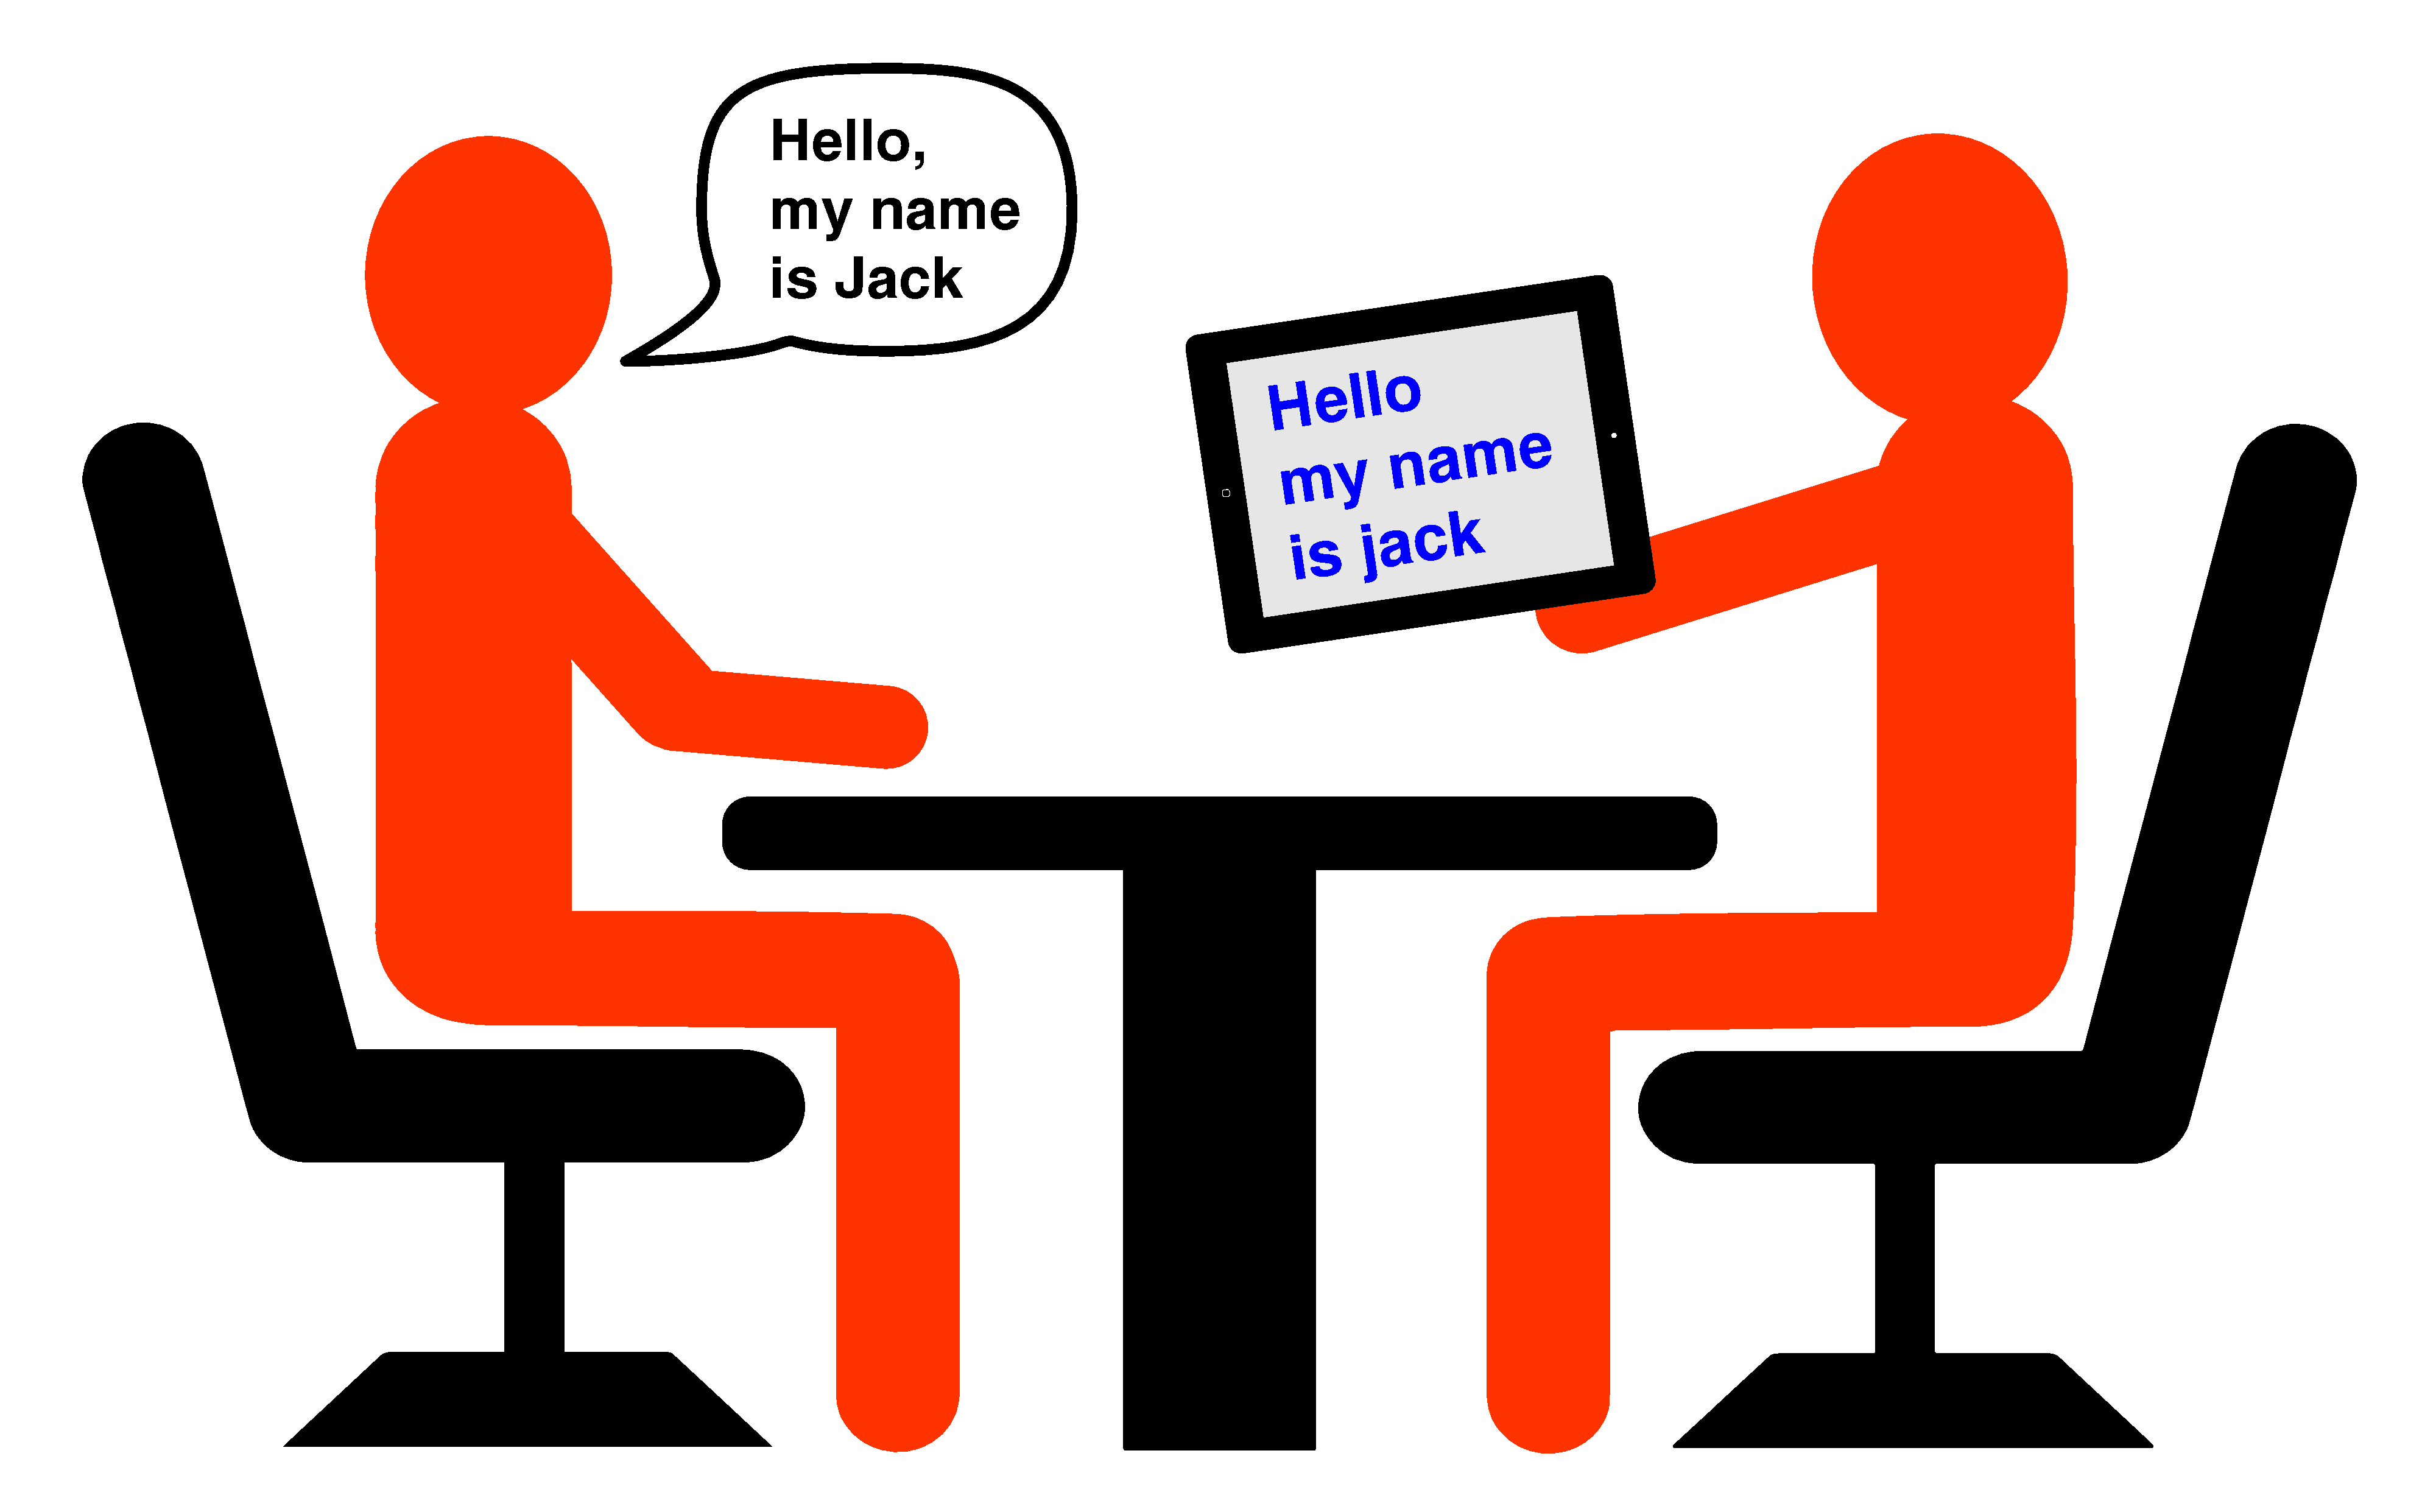
\includegraphics[trim={0cm 0cm 0cm 0cm}, clip, width=\textwidth]{assistant3.pdf}
	\caption{The operation principle and an example use case for the Conversation Assistant. In the picture, the person on the left is speaking. The person on the right uses the Conversation Assistant, which converts that speech into text in real-time.}
	\label{fig:assistant} 
\end{figure} 

\subsection{Problems With Current Solutions}

Some deaf and hard of hearing persons use sign language as an alternative for spoken communication. While this can work well for people who are fluent in it, the problem is that very few people know sign language, especially outside the deaf community. In fact, the share of sign language users among the hearing impaired has been constantly decreasing as a result of modern treatment technology \cite{stacey2006hearing, raino2012sisakorvaistutteen}. In particular, the cochlear implant has enabled a significant share of prelingually\footnote{before language acquisition, including congenital cases (present at birth).} deaf children to not require sign language for communication anymore \cite{moore2007cochlear, peterson2010cochlear}. Different studies estimate that in the near future, approximately 60-80\% of prelingually deaf children will use speech as their main means of communication, as opposed to sign language, thanks to the improved auditory perception provided by cochlear implants \cite{raino2012sisakorvaistutteen}. As a consequence, the need and incentive for the general public to learn sign language in order to communicate with hearing impaired individuals is diminishing even further. As the technological and medical solutions continue to advance, sign language is slowly becoming obsolete. Indeed, sign language is feared and predicted to become extinct in the coming decades \cite{raino2012sisakorvaistutteen}. \\\\
While modern hearing aids and cochlear implants have become very sophisticated by utilizing digital technology and signal processing, there remains many challenges and limitations in their everyday use \cite{levitt2007historical}. One of the major obstacles can be the cost: High-end, personalized devices and surgery are expensive, especially if not covered by health insurance or provided by a public healthcare system \cite{wilson2017global}. Adherence to hearing aid use and rehabilitation can be poor: It has been estimated that only 20-50\% of people who would benefit from a hearing aid are actually using one \cite{koskela2013kuulokojeen}. Even with the extensive digital signal processing and noise reduction in current devices, speech intelligibility in situations with background noise remains one of the major challenges \cite{healy2016difficulty, levitt2007historical, goehring2016speech}. Cochlear implants in particular appear to be very susceptible to noise with a dramatic reduction in speech perception quality in noisy conditions \cite{ healy2016difficulty, friesen2001speech, fu2005noise, srinivasan2013improving}. \\\\
For public spaces and events, the effects of noise and the environment can be alleviated with a specially installed induction loop, commonly referred to as a \textit{hearing loop} \cite{salonen2013hearing}: The desired sound source is fed electrically into a current-carrying wire loop, and the resulting electromagnetic field containing the baseband audio signal is picked up directly by a hearing aid or other device. The pickup coil in a hearing aid or implant is commonly referred to as a \textit{telecoil} (or T-coil). Typical installation locations include airports, auditoriums, concert halls and public bureau buildings. FM systems are a similar alternative for induction loops, which use radio transmission instead of electromagnetic induction. Naturally, these solutions are also not without some technical and practical complications. Interference from metallic structures and other equipment can be an issue, leading to an uneven field strength and affecting the reception quality. One very concrete problem is that many places don't have them installed yet \cite{healy2016difficulty, wilson2017global}. \\
Currently, Human sign and written language interpreters have a large role in facilitating face-to-face communication between hearing and non-hearing persons, especially in more formal situations that can be scheduled in advance \cite{raino2012sisakorvaistutteen, pereira2010communication}. Written language interpreters translate speech to text simultaneously with a speaker by manually typing it into a computer. Written language interpretation happens only in one direction, whereas sign language interpretation can be bidirectional: first, the sign language interpreter translates speech into signs. Then the sign language user can respond with signs, which are then spoken aloud by the translator. Interpreters are used for example in classrooms, meetings, public events and private appointments. Requiring such an extra person for communication has many obvious disadvantages. Firstly, there are the multitude of practical challenges: Interpreters are not available at all times and in all situations. Their number and availability can be quite limited especially outside urban population centers. Professional interpreters typically require a multiyear education and training, limiting their number and introducing costs. Privacy can also be a concern, even though interpreters are customarily bound by confidentiality. \cite{pereira2010communication} \\\\
In conclusion, all the existing traditional solutions have their own problems. One of the fundamental issues with many of these are the costs associated with them, both for the individual and for society \cite{wilson2017global}. Our proposed, automatic speech recognition based solution has the potential to be a relatively inexpensive and highly cost-efficient alternative, enabling communication for the hearing impaired in most everyday situations quickly and conveniently. Ideally, the Conversation Assistant could also remove the need for human interpreters in many situations, or at least function as a workable alternative when human interpreters are not present or available.

\subsection{Research Goals}

A lot of research and progress has been made on improving automatic speech recognition technology \cite{yu2014automatic, gales2008application, keronen2014approaching, hinton2012deep, pylkkonen2013towards, xiong2016achieving, enarvi2017automatic}. While technical advancement and knowledge are valuable purely for their own sake, the practical application of this accumulated knowledge is arguably equally important. Correspondingly, the purpose and contribution of this work is to apply the latest developments in ASR into practice, in the hopes of helping with a real-world problem faced by millions of individuals around the world. \\\\
The main focus of this thesis is on the practical implementation of a proof-of-concept prototype for the Conversation Assistant, as well as user testing the prototype with real users in order to properly validate it as a workable solution. Consequently, designing and performing the necessary user tests for validating the concept and evaluating its usefulness for the end-users also formed a major part of the work. Overall, the contents and research goals of this thesis can be framed into four distinct segments: \\
\begin{enumerate}[itemsep=2.2mm]
	\item Understanding the challenges deaf and hard of hearing individuals face in conversational situations.
	\item Developing a proof-of-concept prototype for use in user testing.
	\item Planning and carrying out user tests with real intended end-users.
	\item Analysing the results:
	\begin{itemize}[align=left,  leftmargin=0.52cm, labelsep=-0.18cm, itemsep=2.2mm]
		\item Is the Conversation Assistant a viable concept, and feasible for practical use?
		\item How it can, and should be, implemented?
		\item What are the main factors for improving its usefulness? 
		\item Is there commercial potential for it? \\
	\end{itemize}
\end{enumerate}

\subsection{Thesis Structure}

This thesis is organized in the following structure: Section \ref{sec:tausta} gives an overview of the foundations of this work, providing background information on hearing impairment, automatic speech recognition, software development and user testing. It also includes a review of previous work relating to this topic and other proposed solutions for the same problem. \\\\
Section \ref{sec:implementation} describes the design and implementation of the Conversation Assistant prototype, including the software tools and libraries used in the programming. Likewise, the models used in our automatic speech recognition system and the data they were trained with are described briefly. \\\\
In section \ref{sec:testing}, the objectives, design quidelines and choices made for the user tests are presented, followed by a detailed description of the resulting test plan and its execution in practice. An objective comparison of the speech recognition models is done, where the models that were used in the user testing prototype are replaced with new, somewhat different models in the hopes of improving the speech recognition accuracy. The results from the user testing are presented and analyzed in section \ref{sec:results}. \\\\
Section \ref{sec:loppu} concludes this thesis. It contains a summary of the work done and results obtained, together with a review whether the objectives set forth in the beginning were met. Finally, conclusions drawn from the results and avenues for future work are discussed.

\clearpage

\section{Background} \label{sec:tausta}

This section presents the theory and scientific context behind the work. Developing and testing the Conversation Assistant is a multidisciplinary task, requiring knowledge from a variety of fields from computer science and engineering to medicine and psychology. Firstly, since we are developing an assistive software-based solution particularly for deaf and hard of hearing individuals, comprehensive knowledge of hearing and hearing loss is required so that the problem being solved can be understood, and the factors affecting it taken into account. Likewise, it is equally important to possess a general overview of currently existing assistive solutions, in order to understand and assess the Conversation Assistants place and impact in the big picture. Information on the social impact of hearing impairment and the problems hearing impaired individuals face on a daily basis offer a clear-cut motivation and reason for the work presented. Additionally, it is relevant to know the demographics of hearing impairment in order to asses the scope of the problem and the scale needed for potential solutions, of which a very concrete example would be how many web servers could potentially be needed for a cloud-based speech recognition application for example in Finland. The number of hearing impaired individuals also directly affects the demand and commercial potential for the presented software solution. Functioning of the Conversation Assistant is based on automatic speech recognition, and therefore, it is necessary to understand how an ASR system works. The main goal of this work is to develop a software application that answers to the needs of the target user group as well as possible. Succeeding in this goal requires the discipline of software engineering, especially in the form of user-centered design and software engineering. Overall, these contents form the theoretical framework enabling the design, engineering and realization of the desired end-result. \\\\
The contents of this section are divided as follows: \ref{subsec:hear} contains a review of hearing impairment, including the physiological mechanisms and societal impact. In addition, existing treatments and assistive technology is covered briefly. \ref{subsec:asr} presents the theory and operation of automatic speech recognition systems, and \ref{subsec:soft} describes the principles of software development, interface design, and user testing as related to this thesis. Previous work relating to this particular topic and other newly proposed technological solutions are reviewed in \ref{subsec:work}.

\subsection{Hearing Impairment} \label{subsec:hear}

Unlike many other disability groups, hearing impaired people are a highly heterogeneous group with different types and levels of hearing impairment \cite{cavender2008hearing}. There are some for whom sign language is their primary, or even possibly their only language, and conversely, there are many who do not know or use sign language at all \cite{raino2012sisakorvaistutteen}. Some are born deaf, while others can suffer from hearing loss later in life due to an illness, accident or through exposure to noise \cite{moore2007cochlear}. Age-related hearing loss is common for the elderly, even though many of them do not identify themselves as hearing impaired \cite{salonen2013hearing}. Typically, the term \textit{hard of hearing} is used to refer to individuals with some degree of hearing still present and communicate mostly through spoken language \cite{deafness}. The term \textit{deaf} most commonly refers to people with very little or no hearing ability at all, often using sign language for communication \cite{deafness}. \\\\
Hearing loss can be an invisible disability, and there remains some social stigma associated with it. Individuals with hearing loss often try to hide it, as it can be perceived to be associated with ageing or low intelligence \cite{wilson2017global, salonen2013hearing}. Access to modern assistive devices and treatment remains limited for many people, even in the developed countries \cite{wilson2017global}: The high cost of hearing aids and cochlear implants means that many people who could benefit from them cannot afford one.

\subsubsection{Definition}

Hearing impairment can be defined as having a reduced or deficient hearing ability, generally caused as a result of decreased hearing sensitivity in one or both ears \cite{moore2007cochlear, ohlenforst2017effects}. Neurological conditions affecting auditory processing in the brain have also been identified, though they are quite rare and hard to diagnose. These \textit{auditory processing disorders} show as various difficulties in recognizing and interpreting sounds correctly, even though the ears are functioning physiologically normally \cite{deafness}. The terms \textit{hearing impairment} and \textit{hearing loss} ar commonly used synonymously \cite{moore2007cochlear}. In this work, \textit{hearing loss} is used to refer specifically to the sensory impairment of hearing, and \textit{hearing impairment} to the overall condition and disability resulting from auditory dysfunction. \\\\
Hearing loss can be divided into two main categories based on the physiological cause \cite{moore2007cochlear, deafness}: Conductive hearing loss is a result of abnormalities in the outer ear or in the ossicles ("hearing bones") in the middle ear, with the effect that sound is not properly transmitted to the inner ear. Sensorineural hearing loss results from a malfunction of the inner ear or the auditory nerve, meaning that the problem is in converting sound vibration into neural impulses and transmitting them to the auditory cortex of the brain. For example, damage to hair cells in the cochlea is a common form of sensorineural hearing loss \cite{moore2007cochlear}. The anatomy of the ear is presented in figure \ref{fig:ear}, describing the parts belonging to the outer, middle, and inner ear. \\\\
The overwhelming majority of all hearing impairments are of the sensorineural type, with age-related hearing loss (\textit{presbycusis}) being the most common cause, followed by noise-induced hearing loss \cite{koskela2013kuulokojeen}. It is possible to have a combination of both conductive and sensorineural hearing defects as well. Another significant division for hearing loss and its treatment is the age of onset in relation to speech acquisition \cite{deafness, raino2012sisakorvaistutteen}: Prelingual hearing loss is present before language acquisition, meaning it is either congenital (present at birth) or develops soon after. Postlingual hearing loss occurs after the development of speech and language. This distinction is important since deafness and hearing loss can significantly affect the language acquisition of children, a fundamental part of general cognitive development \cite{wilson2017global, moore2007cochlear, raino2012sisakorvaistutteen}. \\
\begin{figure}[h]
	\centering 
	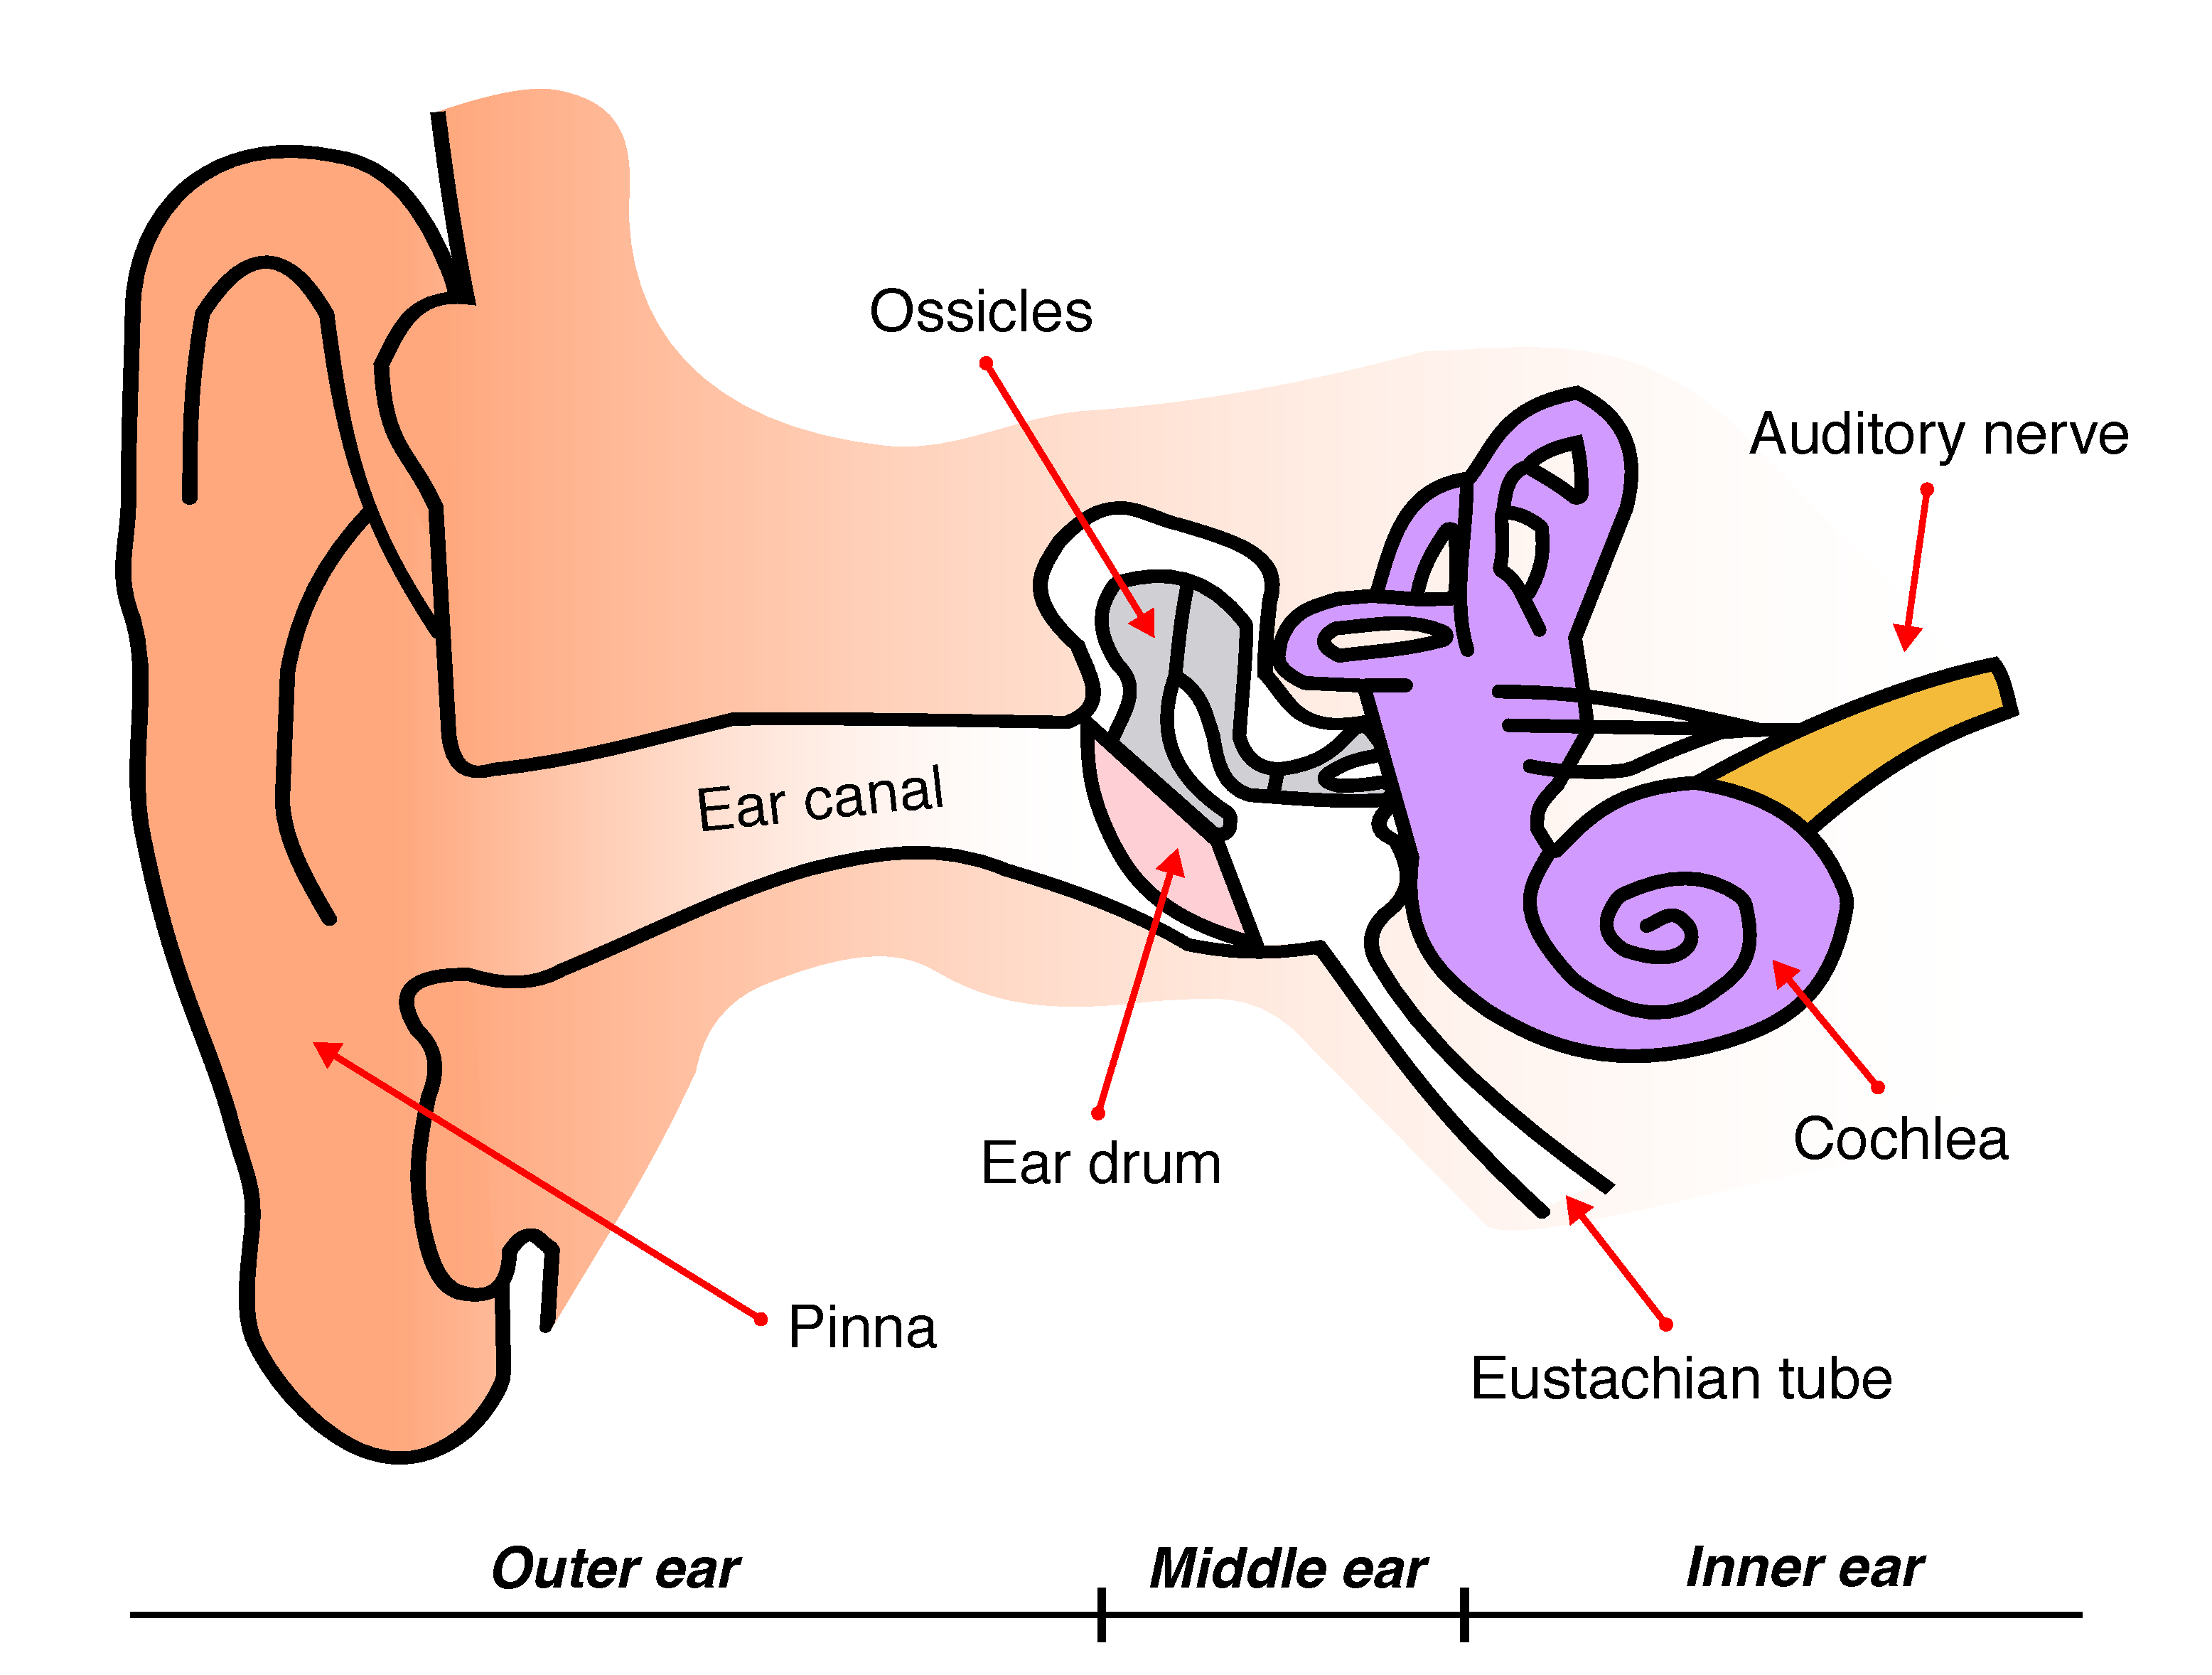
\includegraphics[width=\textwidth]{ear.pdf}
	\caption{Anatomy of the ear. The outer ear consists of the pinna and the ear canal, ending to the eardrum (tympanic membrane). The middle ear is a small air-filled cavity containing the ossicles: three tiny bones responsible for transmitting the vibration of the eardrum to the inner ear. The Eustachian tube is a narrow channel connecting the middle ear to the oral cavity, balancing the air pressure inside to the external air pressure. The inner ear houses the cochlea, a spiral-shaped liquid-filled tube containing the basilar membrane, along which the hair cells are positioned. Hair cells convert the vibration of the basilar membrane into neural impulses in the auditory nerve. \cite{moore2007cochlear, pulkki2015communication}}
	\label{fig:ear} 
\end{figure} \\
Audiologically\footnote{Audiology is the scientific study of hearing, including the treatment of hearing defects.}, hearing loss is categorized and its severity ranked according to the increase in the threshold of hearing, i.e., the sound pressure level required for the perceptual detection of sound \cite{moore2007cochlear}. It is measured in decibels and compared to the statistically defined and standardized nominal level of hearing. Human hearing is strongly frequency-dependent, and is most sensitive at frequencies from approximately one to five kilohertz \cite{pulkki2015communication}. Consequently, this frequency range is critical for speech perception and many other everyday tasks. \\\\ Figure \ref{fig:loudness} presents the equal-loudness contours (curves) as they are defined in the ISO 226:2003 standard \cite{iso226}. These contours describe the \textit{sound pressure level} (SPL) required for a pure tone (single frequency sinusoidal waveform) to be judged equally loud depending on the frequency of the tone, illustrating the frequency-dependent sensitivity of hearing \cite{pulkki2015communication}. Notably, the equal-loudness curve for zero phons corresponds to the absolute threshold of hearing. Hearing loss can therefore be technically defined as upward changes to this curve, the frequency-dependent threshold of hearing, that exceed the normal small statistical variation between different persons. \\
\begin{figure}[]
	\centering 
	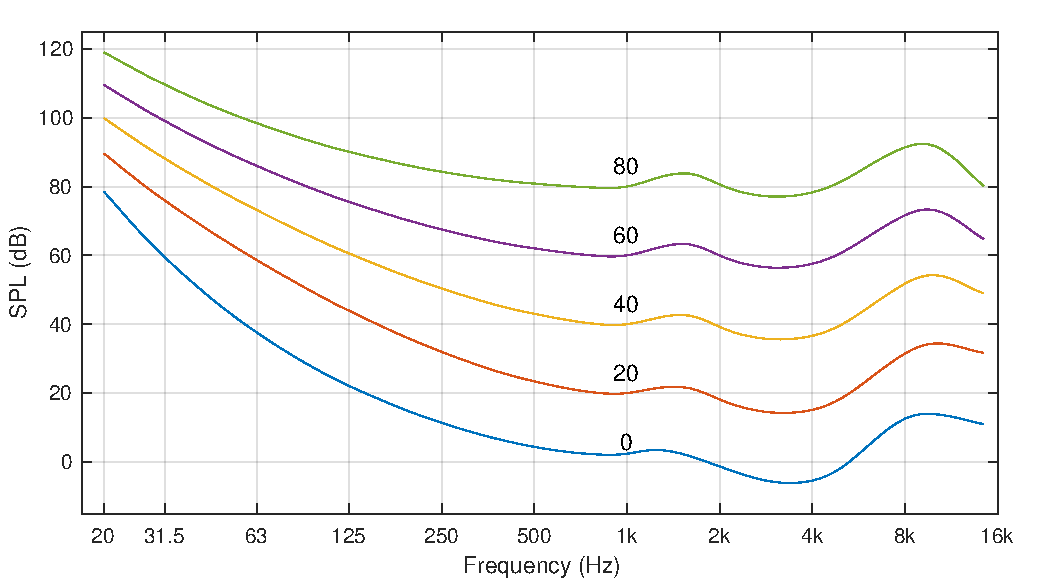
\includegraphics[width=\textwidth]{loudness.pdf}
	\caption{Equal-loudness contours as defined in ISO 226:2003. The number associated with each curve is the nominal loudness level in phons, with zero phons corresponding to the nominal threshold of hearing. Sound pressure level is the pressure level compared to the reference value of \ $ \mathit{20 \cdot 10^{-6}}$ Pascals. \cite{iso226}}
	\label{fig:loudness} 
\end{figure} \\
The level of hearing loss is generally described as a single decibel value, referred to as the \textit{pure tone average} (PTA) \cite{moore2007cochlear, salonen2013hearing}. It is calculated as the average of the hearing thresholds for pure tones at the frequencies of 0,5 kHz, 1 kHz, 2 kHz, and 4 kHz: For each frequency, the threshold of hearing is measured and compared to the reference value, resulting in a decibel value, which are then averaged together to form a single value estimate. Different severity categories have been set up with each category having a corresponding decibel range of the average hearing threshold increase. These decibel ranges vary slightly between countries and organizations \cite{salonen2013hearing}. Table \ref{table:hearingloss} presents the common severity ranks, and the corresponding decibel ranges for the pure tone average used by the \textit{World Health Organization} (WHO) and the \textit{European Working Group on Genetics of Hearing Impairment} (EUWG) \cite{salonen2013hearing}. \\\\
However, this does not mean that all individuals in the same category or even with the same pure tone average value have the same effective hearing impairment: Difficulties for instance with speech perception can vary widely depending on how much each frequency is affected and the mechanisms causing the hearing loss. People with mild or moderate hearing loss can typically understand speech reasonably well in a quiet room with only one person talking. However, they can start having difficulties when more than one person is talking at the same time, or when there is background noise or notable reverberation present \cite{peterson2010cochlear}. People with severe or profound hearing loss usually have difficulties even with understanding a single speaker in a quiet room, and severe problems when background noise is present. In addition to decreased audibility, hearing impairment typically causes additional perceptual difficulties not purely related to the reduced sensitivity \cite{moore2007cochlear}: The frequency resolution of hearing is often also affected, leading to the significant difficulties with speech perception in noisy conditions. \\\\
Normally, humans are very good at understanding speech in noise and can concentrate on a specific speaker or audio source among many other competing sources. This is typically referred to as the \textit{cocktail party effect} \cite{bronkhorst2000cocktail}. In hearing loss, the auditory filters of the ear that divide the incoming sound into different frequency bands can become wider and more shallow due to damage to the (outer) hair cells \cite{moore2007cochlear}. This leads to increased auditory masking of adjacent frequencies, where one sound interferes with the detection of another sound. Also, the level of hearing loss typically varies between the ears, with one ear being better than the other. This affects the binaural processing done by the ear, which is important for sound localization, i.e., the detection of the direction and distance of sound sources \cite{moore2007cochlear, pulkki2015communication}. The end result is that the auditory system is unable to effectively isolate speech from noise, meaning that simply amplifying all sound does not help \cite[p.~233--234]{moore2007cochlear}. Instead, the \textit{signal-to-noise ratio} (SNR), the ratio between the level of the desired audio signal and the level of the background noise, needs to be improved considerably for better speech intelligibility in noisy conditions \cite{healy2016difficulty, fink2008benefit}.
\begin{table}[t]
	\renewcommand{\arraystretch}{1.2}  % set row height to 1.2x default
	\setlength{\tabcolsep}{32pt}                % set space between text and cell border
	\centering
	\caption{Categories for the grade of hearing loss and corresponding pure tone average ranges as defined by WHO and EUWG \cite{salonen2013hearing}.}
	\label{table:hearingloss}
	\begin{tabular}{@{}lll@{}}
		\toprule
		& \textbf{WHO}        & \textbf{EUWG}        							\\ \midrule
		Severity 	& \multicolumn{2}{l}{Pure Tone Average (dB HL)} 	 \\ \midrule
		Normal   	& 0-25                		& 0-19                 					\\
		Mild     		& 26-40               		& 20-39                				\\
		Moderate 	& 41-60               		& 40-69                				\\
		Severe   		& 61-80               		& 70-94                				\\
		Profound 		& $\geqslant$ 81        & $\geqslant$ 95         \\ \bottomrule
	\end{tabular}
	\vspace{2mm}
\end{table}

\subsubsection{Prevalence}

In this case, prevalence is defined as the percentage of a population that is affected by hearing loss. A pure tone average greater than 25 dB HL in both ears is defined as disabling hearing loss by WHO criteria, as exceeding this level begins to clearly impair communication in daily life \cite{salonen2013hearing}. Most population studies use this number for defining hearing impairment \cite{salonen2013hearing, lin2011hearing}. From a public health perspective,  hearing impairment can be considered a major health and economic problem: approximately 0,1 - 0,3\% of newborn children have hearing impairment, while over 50 percent of the population over 75 years of age has a hearing loss requiring treatment \cite{salonen2013hearing}.  \\\\
In Finland, an estimated 11 percent of the workforce and around 15-18\% of the whole adult population has some degree of hearing loss \cite{koskela2013kuulokojeen, salonen2013hearing}. The prevalence of hearing impairment among the elderly is high: A Finnish study with 4067 participants found that for the age groups 70, 75, 80, and 85 years, the prevalence for at least mild hearing loss varied between 37,7\% - 54,1\%, and between 21,1\% - 38,9\% for moderate or more severe hearing loss \cite{salonen2013hearing}. Among this group, hearing aids were used daily by 55,4\% of the 249 persons who responded to a mailed interview. \\\\
In the USA, Lin et al. \cite{lin2011hearing} estimated in 2011, based on data from 2001 to 2008, that 30.0 million or 12.7\% of Americans aged 12 years or older had bilateral hearing loss, increasing to 48.1 million or 20.3\% when individuals with unilateral hearing loss were included. Overall, they found hearing loss to increase with every age decade, with the prevalence of hearing loss expected to rise because of an aging population. \\\\
According to the Global Burden of Disease study of 2015 \cite{wilson2017global}, approximately half a billion people have disabling hearing loss globally, which corresponds to 6,8\% of the whole world's population. Wilson et al. \cite{wilson2017global} report that these numbers are substantially higher than estimates published before 2013, pointing to the growing importance of hearing loss as a disability, and the need for greater attention to global hearing health care.

\subsubsection{Assistive Devices}

The main technological solutions to hearing loss can be divided into three main categories: hearing aids, cochlear implants, and other assistive devices \cite{moore2007cochlear}. Hearing aids are used in mild to severe cases to augment a reduced hearing ability \cite{moore2007cochlear, levitt2007historical}. A cochlear implant is required when hearing aids cannot help anymore, in cases of profound or total hearing loss \cite{moore2007cochlear, levitt2007historical}. Other assistive devices include both supplementary techniques for hearing augmentation, and a wide variety of methods and gadgets based on visual perception and physical interaction. For additional hearing assistance, the previously mentioned audio induction loop and FM system are the most common and widely used, and many hearing aids and cochlear implants have a build-in receiver for these devices. Examples of the latter category include alarm systems using flashing lights instead of sound for applications such as smoke detectors and door bells. A typical example of an assistive device substituting sound with physical interaction is an alarm clock using vibration for awaking a deaf person. Hearings aids and cochlear implants are being actively developed, and have improved remarkably during the past few decades, though neither device can match the performance of normal hearing \cite{moore2007cochlear, levitt2007historical, goehring2016speech}. More traditional support methods are still being used as well: Lip reading is utilized by many hearing impaired individuals for understanding speech in conjunction with the devices. \\\\
Hearing aids are used to amplify and modify incoming sound, enhancing and augmenting the users own compromised hearing \cite{levitt2007historical, salonen2013hearing, fink2008benefit}. Modern devices are based on digital electronics and microprocessors, and come in many different types. The most common variations are the different \textit{in-the-ear} and \textit{behind-the-ear} models. Figure \ref{fig:hearingaids} presents various types of modern hearings aids from one particular manufacturer (Widex). \\
\begin{figure}[h]
	\centering 
	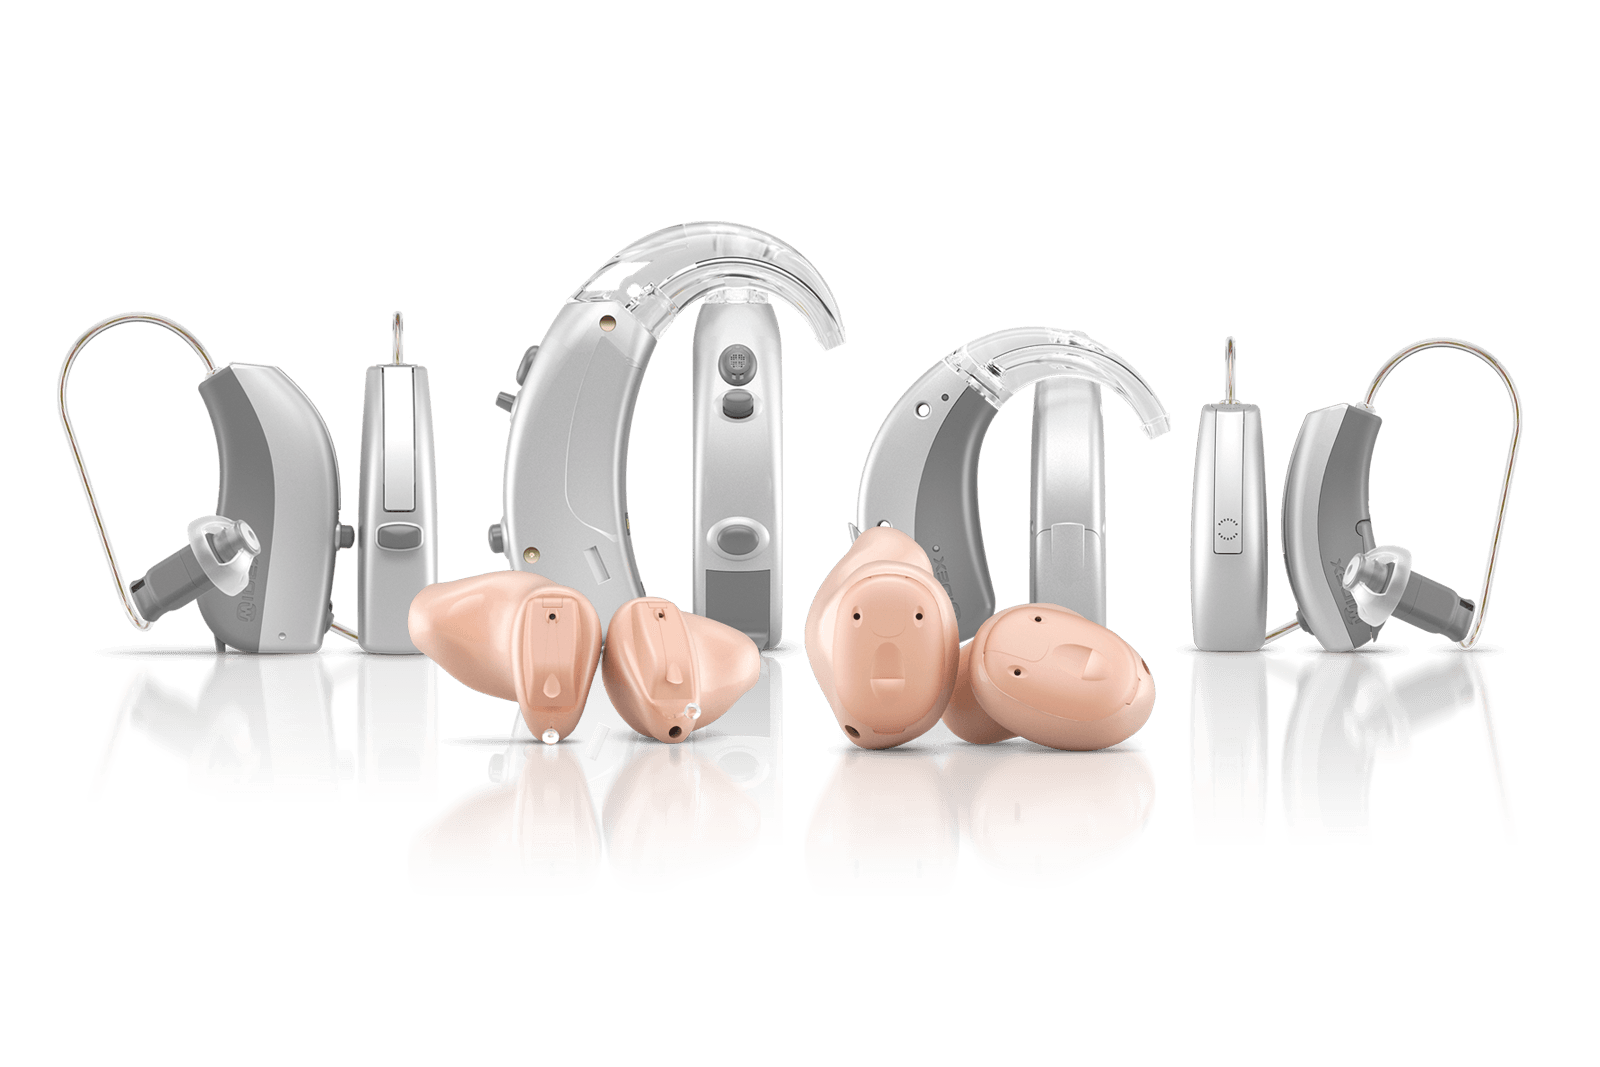
\includegraphics[trim={0cm 4cm 0cm 4cm}, clip, width=\textwidth]{hearingaids.png} 	% trim={<left> <lower> <right> <upper>}
	\caption{Different types of modern hearing aids: behind-the-ear (back, middle), receiver-in-canal (back, left and rightmost), in-the-canal (front, left) and in-the-ear (front, right). Image source: \href{https://www.widex.pro/en/products/unique-hearing-aids}{\textit{Widex}}}
	\label{fig:hearingaids} 
\end{figure} \\
In addition to the simple amplification provided by earlier analog models, modern digital hearing aids utilize real-time \textit{digital signal processing} (DSP) for tasks such as speech enhancement, dynamics processing (compression), filtering, noise reduction, adaptive gain control and feedback cancellation \cite{moore2007cochlear, levitt2007historical, goehring2016speech}. Directional microphone systems are used for improving speech recognition in noise. Modern wireless transmission technology, such as Bluetooth, can be used to easily link hearing aids directly with sound sources like a telephone or television \cite{salonen2013hearing}. Modern hearing aids are personally fitted for each user, matching and compensating for the individual frequency response of the users hearing for best results \cite{moore2007cochlear}. \\\\
A cochlear implant is a surgically implanted device that can provide auditory perception to people with severe or profound sensorineural hearing loss, even in the case of complete deafness \cite{moore2007cochlear, peterson2010cochlear}. Cochlear implants bypass the ear altogether by directly stimulating the auditory nerve with electrical signals through electrodes inserted into the cochlea. All implants are comprised of two major elements: The external, detachable parts, and the internal, surgically implanted parts. The external parts are usually removed for activities such as sleeping and bathing \cite{peterson2010cochlear}. \\\\
Similarly to hearing aids, the audio signal is acquired with an external microphone or picked up wirelessly. The signal is processed with a speech processor typically worn behind the ear. It is then transmitted wirelessly through the skin to the internal implant. The internal implant part consists of a receiver and the electrodes. The placement of these components is illustrated in figure \ref{fig:implant}, which presents the same anatomic view of the ear as in figure \ref{fig:ear}, but with an added cochlear implant: \\
\begin{figure}[h]
	\centering 
	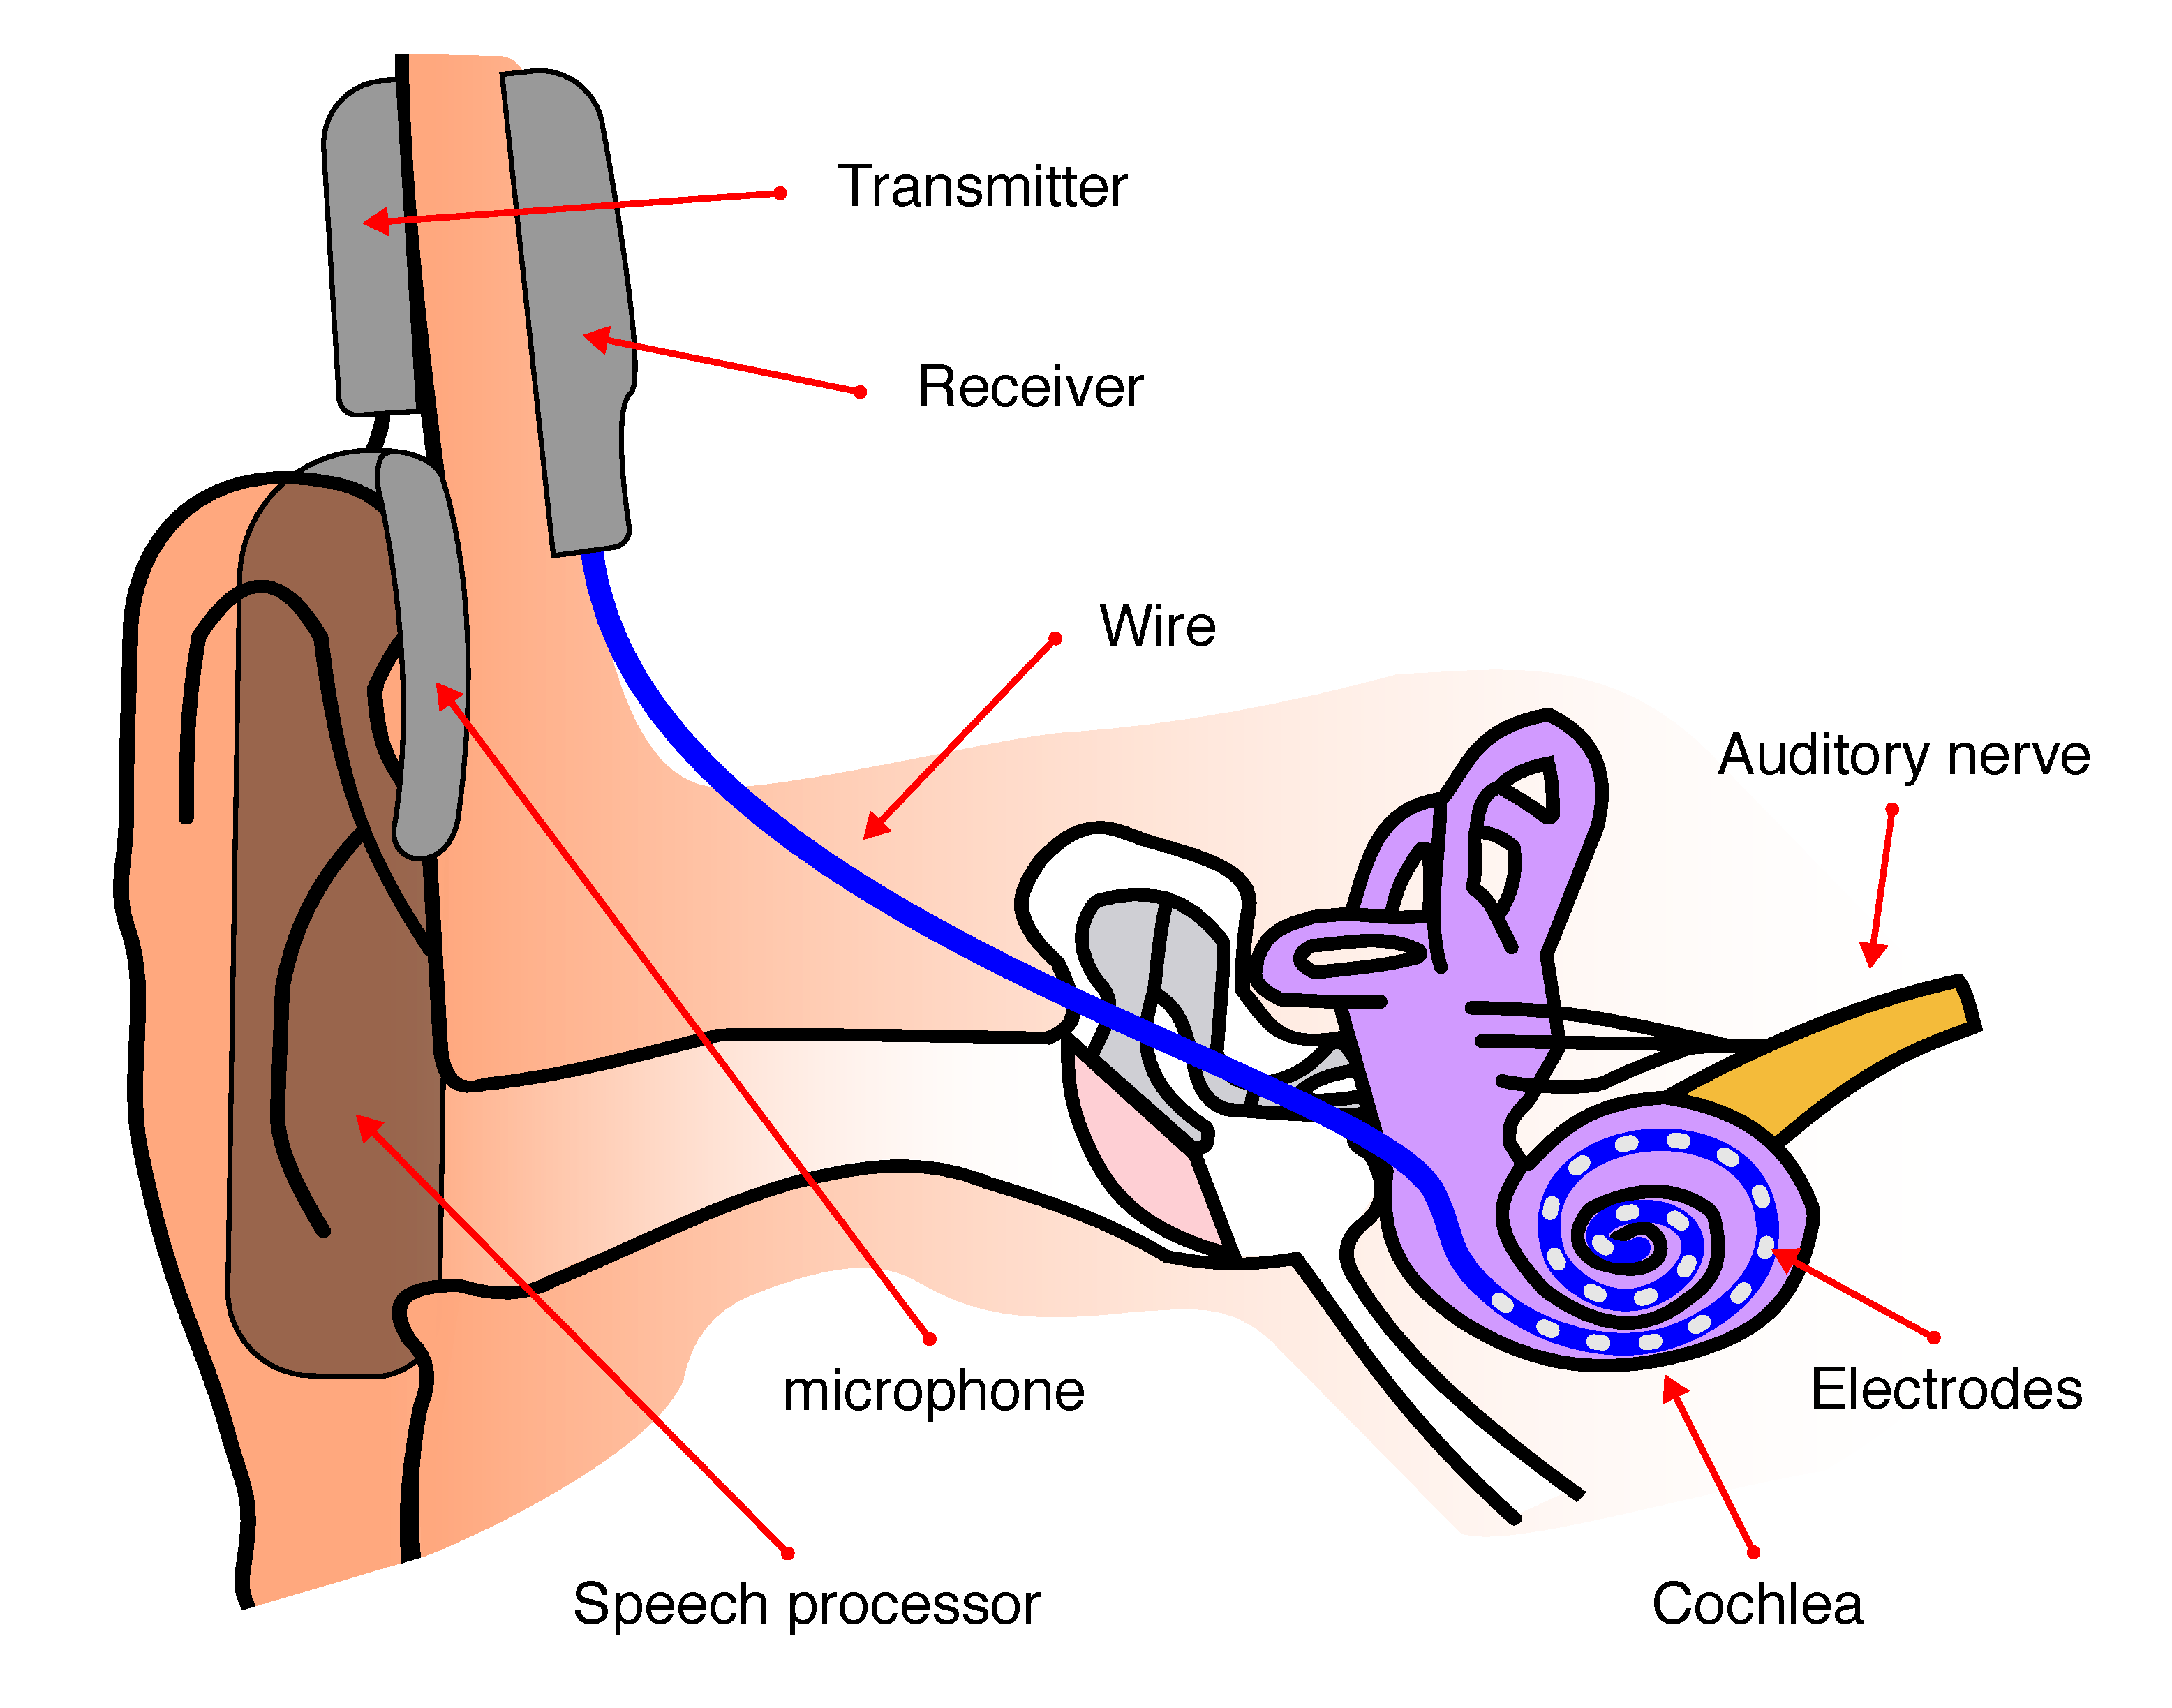
\includegraphics[width=\textwidth]{implant.pdf}
	\vspace{0.5mm}
	\caption{An ear with a cochlear implant. A microphone and speech processor are typically worn behind ear. The speech processor connects to a wireless transmitter attached outside the head. An internal receiver inside the skin connects to the electrodes inserted into the cochlea. \cite{moore2007cochlear, peterson2010cochlear}}
	\label{fig:implant} 
\end{figure} \\
Most cochlear implants are multi-channel, meaning they have multiple electrodes. The input signal is likewise divided into multiple frequency bands with each electrode receiving its own signal \cite{moore2007cochlear, friesen2001speech}. While they do not restore normal hearing sensation, cochlear implants enable speech communication for many recipients and significantly improve the spoken language acquisition for deaf children \cite{stacey2006hearing, raino2012sisakorvaistutteen}: Many congenitally deaf cochlear implant recipients achieve a good speech perception ability and develop near-normal language skills. Post-lingually deafened implant recipients often regain the ability to understand and use spoken language at least to some degree. Cochlear implants have been shown to considerably improve the perceived quality of life for many recipients \cite{blomberg2012sisakorvaistutetta}. \\\\
Cochlear implants are a relatively new treatment method: In Finland, the first few implants were installed in the mid 80s to adults. The first child was implanted in 1995 and the first congenitally deaf child in 1997 \cite{raino2012sisakorvaistutteen}. Today, the majority of prelingually deaf children are implanted already at the age of one, as the age of implantation is strongly associated with successful outcomes \cite{peterson2010cochlear, stacey2006hearing, raino2012sisakorvaistutteen}.

\subsubsection{Social impact}

Hearing loss can cause profound social problems and greatly affect an individuals physical and psychological well-being as a consequence of the difficulty with communication and social interaction. \cite{wilson2017global, koskela2013kuulokojeen}. The effects of hearing loss can lead to social isolation and stigmatization, depression, and problems with self esteem and work capacity \cite{wilson2017global, koskela2013kuulokojeen, lavikainen2014}. Coping with hearing loss can be challenging, and consequently, psychological illnesses have been found to be more prevalent for the hearing impaired than for those in the general population \cite{wilson2017global}. On a personal level, the quality of life of an individual is ultimately impacted \cite{blomberg2012sisakorvaistutetta}. From a societal and public economy viewpoint, the consequences of hearing loss appear as productivity losses, employment issues, health care and social benefit expenditures, and reduced tax revenue  \cite{wilson2017global}. \\\\
Employment issues is one of the major obstacles hearing impaired people face in society \cite{hietala2008huonokuuloinen}. In Finland, the unemployment rate of people with hearing impairment varied from 30 to 40 percent between the years 1995 and 2002 \cite{hietala2008huonokuuloinen}. For young adults with hearing impairment, the unemployment rate was reported to be twice the rate of the normally hearing population in the same age group \cite{hietala2008huonokuuloinen}. \\\\
Employed hearing impaired people have been observed to have noticeable problems with coping at work and workplace well-being \cite{wilson2017global, hietala2008huonokuuloinen}. The increased listening effort associated with hearing loss, particularly in noisy environments, can be tiring and cause stress \cite{ohlenforst2017effects, koskela2013kuulokojeen}. The negative effects of hearing loss are focused particularly to the aging workforce \cite{koskela2013kuulokojeen}. Consequently, there appears to be a clear statistical connection between hearing loss and early retirement \cite{hietala2008huonokuuloinen}.

\clearpage

\subsection{Automatic Speech Recognition} \label{subsec:asr}

In this work, the primary interest in automatic speech recognition is in using it in practice, instead of developing or improving upon some aspect of it. Therefore, this section focuses on providing a high-level, short overview of ASR systems. Likewise, detailed description of machine learning techniques and training methods fall outside this thesis. The focus in this thesis is on modern large vocabulary continuous speech recognition. \\\\ An automatic speech recognition system takes an audio signal containing speech as an input, and tries to produce the corresponding text representation \cite{huang2001spoken, li2014overview}. Figure \ref{fig:asr} presents the high-level block diagram of a typical speech recognition system, though other configurations are also possible. In practice, the actual implementation can in many cases contain more complicated connections between the different components, and the models can be packed together for optimization reasons \cite{yu2014automatic, kallasjoki2016}. The use of deep neural networks has also somewhat blurred the line between feature extraction and acoustic modeling \cite{hinton2012deep, kallasjoki2016}. \\
\begin{figure}[h]
	\centering 
	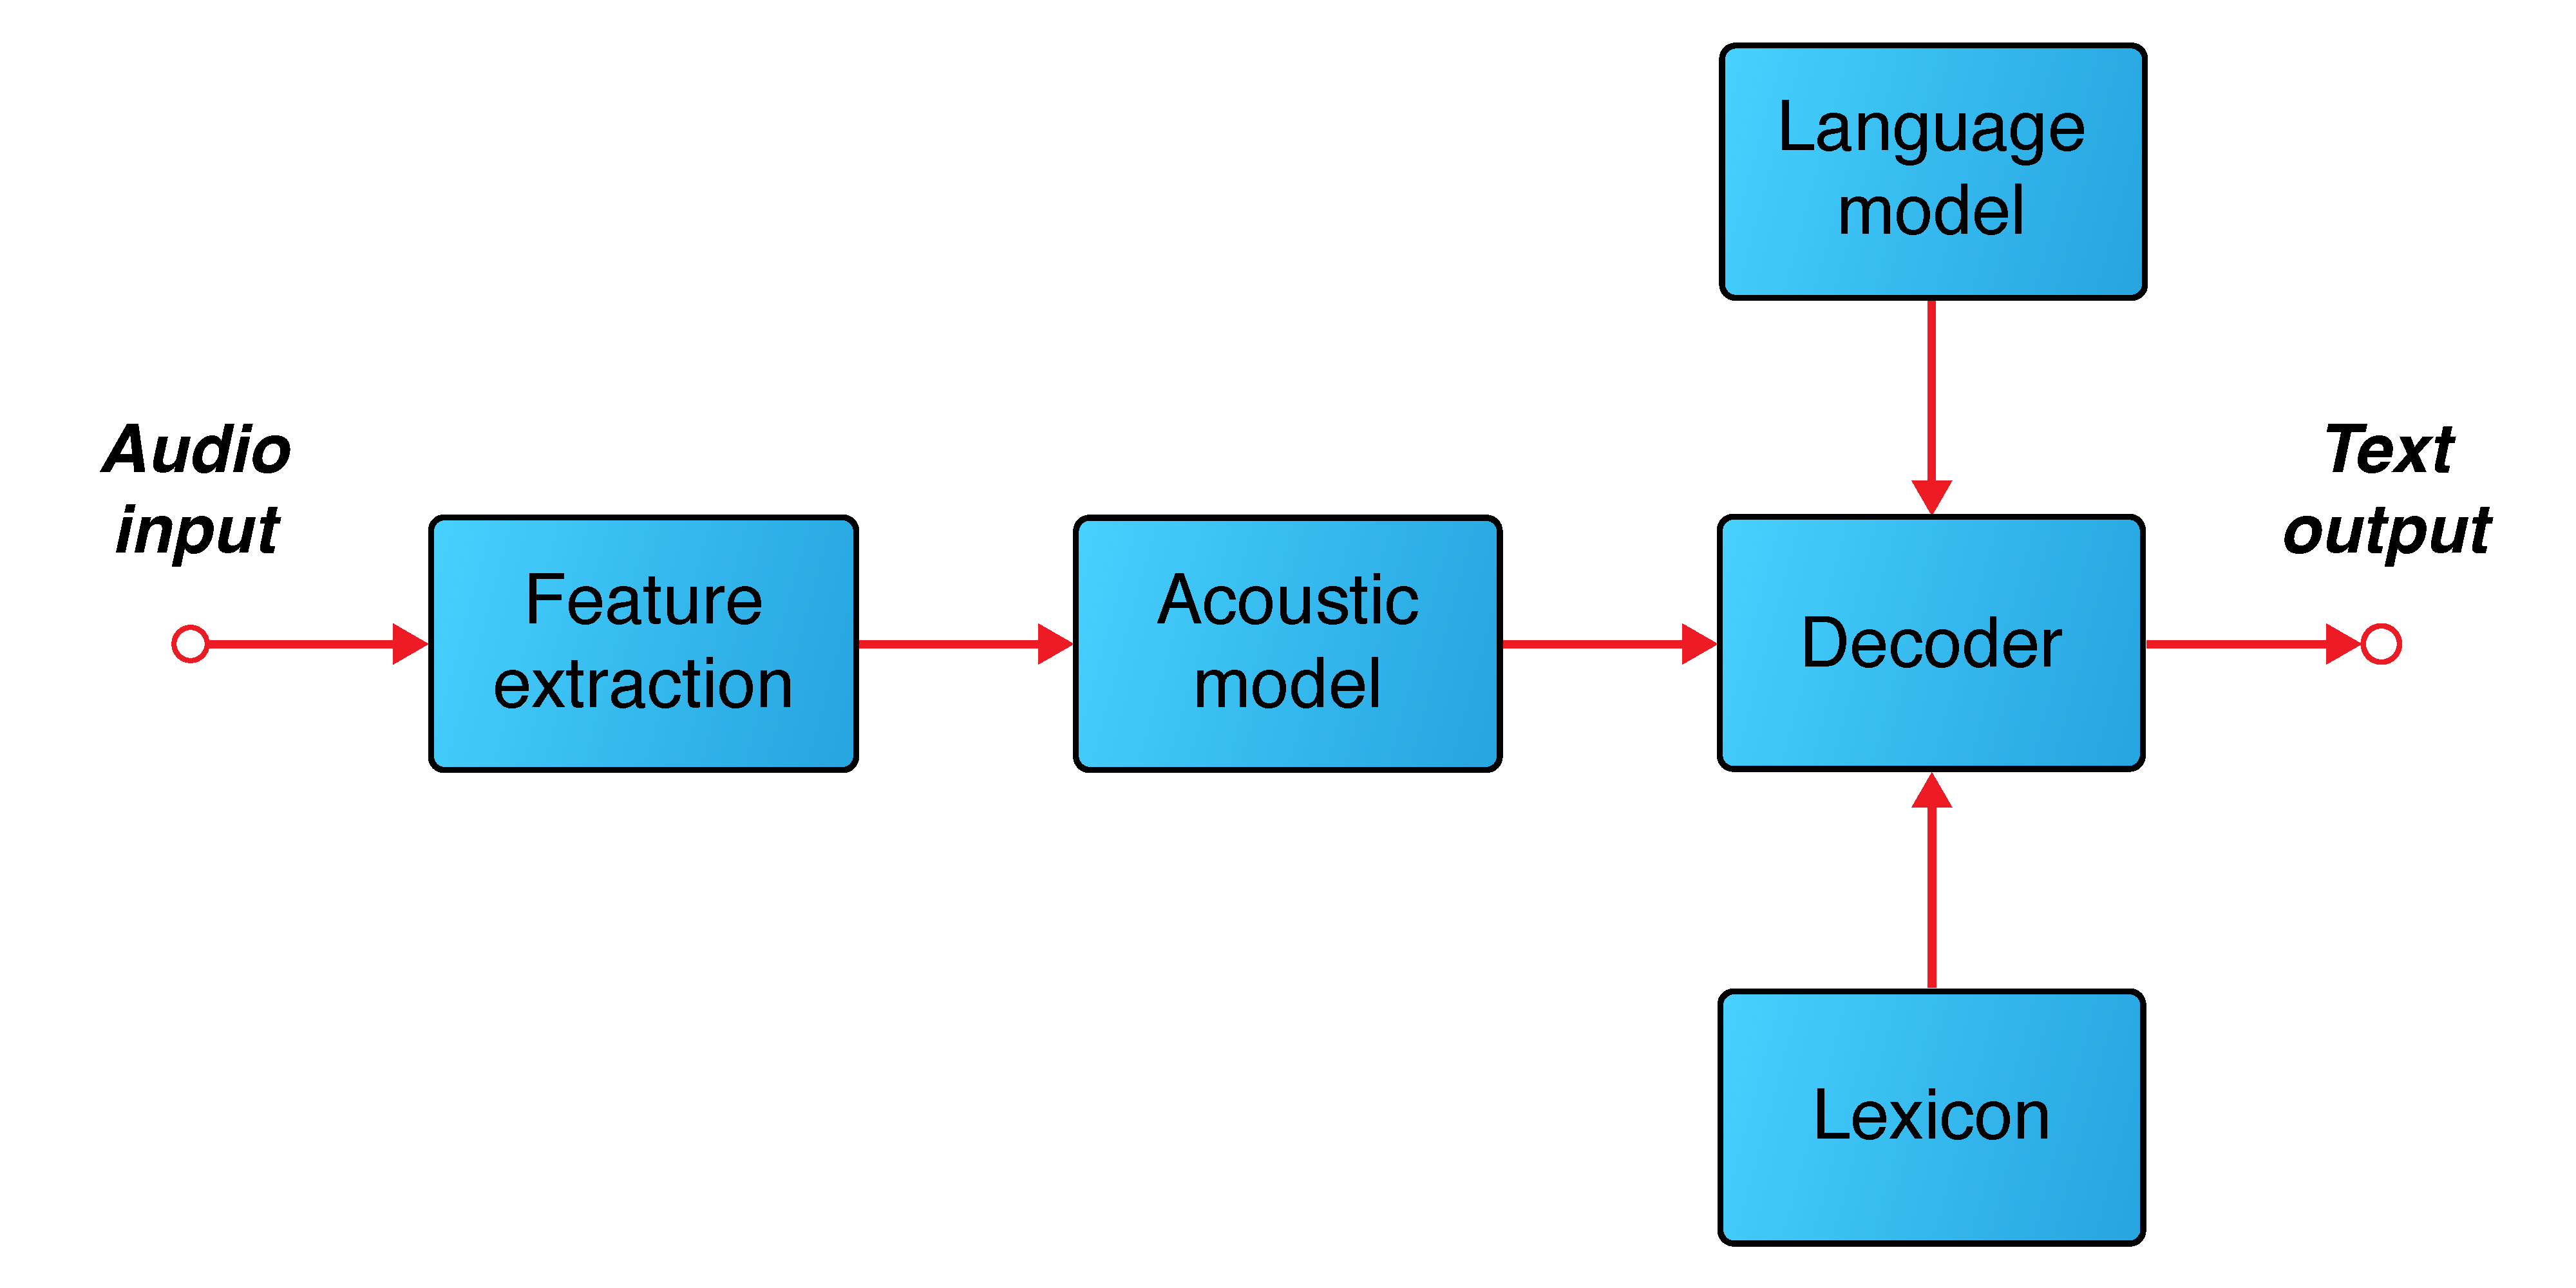
\includegraphics[trim={1.8cm 0cm 1.8cm 0cm}, clip, width=\textwidth]{ASR.pdf}
	\caption{Block diagram for the structure of a typical speech recognition system.}
	\label{fig:asr} 
\end{figure} \\
At the technical level, automatic speech recognition is a conversion process, where an acoustic data sequence (speech) is converted into a symbolic character sequence (text) \cite{yu2014automatic}. In statistical terms, speech recognition can be categorized as a classification problem among the wider context of general pattern recognition tasks \cite{huang2001spoken}. The speech recognition process can be formulated mathematically in the following way \cite{huang2001spoken, gales2008application, kallasjoki2016}: the goal of the system is to produce the word sequence $ \hat{\bm{W}} = w_1, w_2, w_3,\dots,w_n$, for a given acoustic observation sequence $\bm{O}$. The most probable word sequence corresponding to $\bm{O}$ can be found by maximizing the posterior (i.e., conditional) probability $P(\bm{W} | \bm{O})$:
\begin{equation} \label{eq:max}
\hat{\bm{W}} \ = \ \underset{\bm{W}}{\argmax} \ P(\bm{W} | \bm{O})
\end{equation}
However, $P(\bm{W} | \bm{O})$ is difficult to calculate directly \cite{gales2008application}, but it can be transformed into a form that is easier to model statistically. The Bayes' theorem states that \cite[p.~10]{hori2013speech}:
\begin{equation}
P(A | B) \ = \ \frac{P(B | A) \ P(A)}{P(B)}
\end{equation}
With the Bayes' theorem, the probability $P(\bm{W} | \bm{O})$ can be transformed to the equivalent probability:
\begin{equation} \label{eq:max2}
P(\bm{W} | \bm{O}) \ = \ \frac{P(\bm{O} | \bm{W}) \ P(\bm{W})}{P(\bm{O})}
\end{equation}
For finding the maximum, the denominator in equation (\ref{eq:max2}) can be discarded as it stays constant, and equation (\ref{eq:max}) becomes:
\begin{equation} \label{eq:max3}
\hat{\bm{W}} \ = \ \underset{\bm{W}}{\argmax} \ P(\bm{O} | \bm{W}) \ P(\bm{W})
\end{equation}
Here, $P(\bm{O} | \bm{W})$ is the probability of an acoustic observation sequence for a specific word sequence, corresponding to the acoustic model. $P(\bm{W})$ is the probability of a specific word or word sequence occurring, which is given by the language model. In practice, the probability product is often calculated as an addition in the logarithmic domain, with an additional weight $\alpha$ for controlling how much weight is given to the language model \cite[p.~200]{gales2008application}:
\begin{equation}
\hat{\bm{W}} \ = \ \underset{\bm{W}}{\argmax} \big\{ \log P(\bm{O} | \bm{W}) \ + \ \alpha \log P(\bm{W}) \big\}
\end{equation} \\
The following subsections present a brief review of each individual part of the speech recognition process presented in figure \ref{fig:asr}. In other words, how solving equation (\ref{eq:max3}) is implemented in practice.

\subsubsection{Feature extraction}

The input to an ASR system is a digital audio signal, the digitized version of an acoustic sound wave and comprised of discrete samples \cite{yu2014automatic, huang2001spoken}. Figure \ref{fig:audio} presents the waveform and the spectrogram for a short speech sample. The spectrogram is the magnitude spectrum of a signal as a function of time, describing how the frequency contents vary temporally.
\begin{figure}[t]
	\centering
	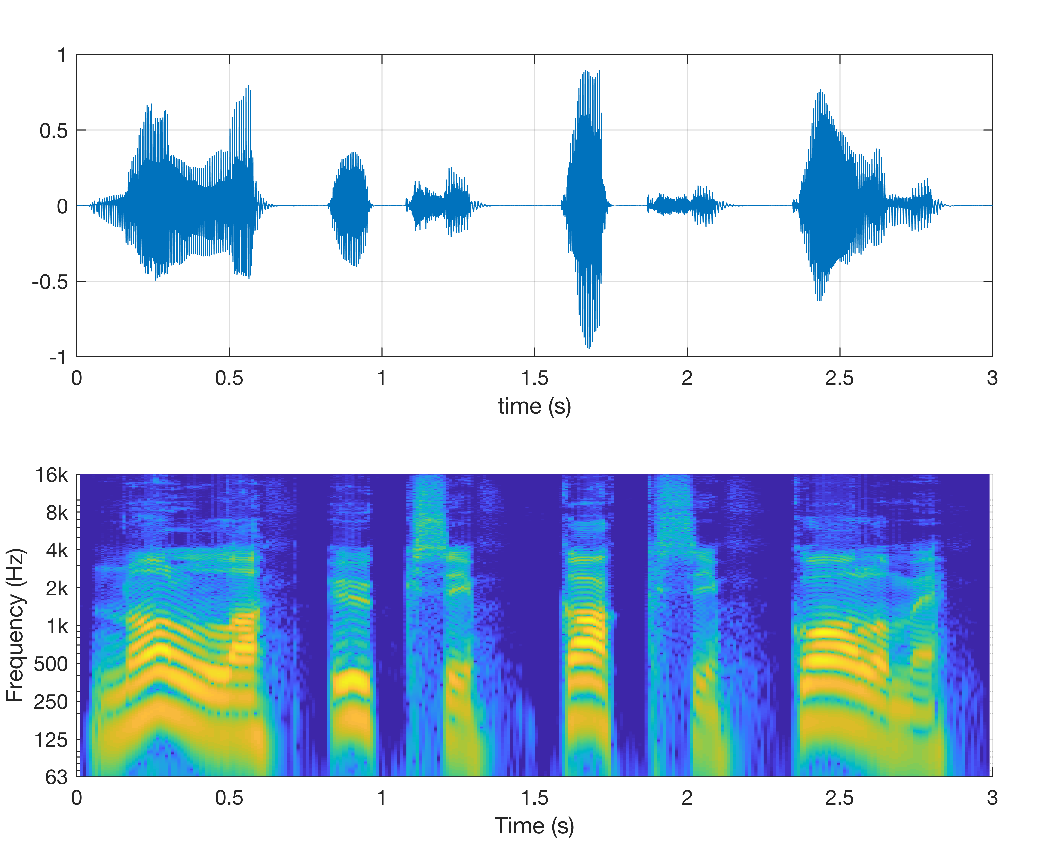
\includegraphics[trim={0cm 0.3cm 0.4cm 0.5cm}, clip, width=\textwidth]{audio.pdf}
	\caption{The waveform and corresponding spectrogram of a speech signal containing the words "zero, one, two, three" pronounced in Finnish.}
	\label{fig:audio} 
\end{figure} 
An audio signal contains acoustic information, such as the energy and frequency of its components. But in ASR, we are interested in the linguistic information. Therefore, the acoustic properties of an audio sample need to be somehow mapped to linguistic information. However, the problem with recognizing speech sounds is that every person has an unique voice, meaning that the same word or sentence spoken by different persons produce widely varying acoustic information contents. These depend for example on the speakers gender, pronunciation, intonation, tone of voice, mood, and characteristic pitch and timbre. The voice of a one specific individual does not stay constant either, and can vary noticeably between different times and situations. Also, in addition to the speech signal of interest, all real-world signals contain some degree of background noise and other unwanted sounds from the recording environment \cite{huang2001spoken}. Therefore, the acoustic properties of a speech sample cannot be used directly. \\\\
What is needed are some characteristic measures, or \textit{features}, that can describe and discriminate between different speech sounds, and extract the linguistic information independent of the speakers personal voice. These features should contain the essential information and measurements needed for classifying speech. \textit{Feature extraction} is then the process of calculating a sequence of these features, a \textit{feature vector}, based on the input audio signal. Ideally, a feature vector should be compact, containing only the necessary information, be robust against noise, as well as fast to calculate so that it can be used in real-time \cite{huang2001spoken}. Consequently, audio signals typically contain a lot of information that is not useful for this particular task. In feature extraction, the input signal is therefore processed to remove unwanted and redundant information as well as noise, while emphasizing the important characteristics. \\
Common preprocessing steps include filtering the signal: The very low and high frequencies can generally be removed as speech is mostly focused between the frequencies from 100 to 4000 Hz. The input is often downsampled to a lower sampling rate, effectively removing unnecessary high frequencies as all frequencies above the Nyquist limit are lost. In practice, sampling rates as low as 8 kHz can be used, limiting the highest possible frequency to just 4 kHz, without a noticeably reduced recognition accuracy \cite{huang2001spoken}. A pre-emphasis filter can be used to adjust the spectral tilt \cite{kallasjoki2016}. The signal is divided into partially overlapping frames, typically around 20 to 30 milliseconds in length, so that the frequency content of each frame can be expected to be fairly stationary \cite{huang2001spoken, gales2008application}. \\\\
\textit{Mel-frequency cepstral coefficients} (MFCC) has been a very popular choice for the feature representation type \cite{yu2014automatic, gales2008application, kallasjoki2016}. It is used because of its capacity for eliminating the speaker dependent characteristics of speech and for matching well to the logarithmic loudness and pitch perception of humans. The mel scale (short for \textit{melody}) is a psychoacoustic frequency scale, where the change in pitch is judged to be perceptually equal in distance on the scale \cite[p.~174]{pulkki2015communication}. Compared to the objective frequency scale in hertz, the mel scale puts more emphasis on low frequencies below one kilohertz, and conversely, compresses higher frequencies as the interval between perceptually equal pitch increments starts to increase exponentially with the frequency in hertz. The mel scale is used in order to better match the non-linear properties of human hearing, accentuating the frequency bands that are more important for human auditory perception. A common formula for converting a frequency in hertz to the mel scale is:
\begin{equation} \label{eq:mel}
m \ = \ 2595 \  \cdot \ \log_{10} \ \left(1 \ + \ \frac{f}{700} \right),
\end{equation} where $f$ is the frequency in Hertz. The anchor point is set to 1000 Hz $\leftrightarrow$ 1000 mel \cite[p.~174--175]{pulkki2015communication}. As we are interested in the frequency contents of the signal, each frame is windowed and converted to the frequency domain by calculating the short-time power spectrum \cite{gales2008application}. A mel-scale filter bank with triangular band-pass filters spaced in perceptually equally long frequency bands is applied to each frame. A mel-scale filter bank is presented in figure \ref{fig:melbank}. The combined energy of each frequency band is then calculated. Finally, the cepstral coefficients are obtained by first taking the logarithm of each energy band, mimicking the logarithmic loudness perception of hearing, and applying the discrete cosine transform, in effect compressing and decorrelating the energies \cite{huang2001spoken, gales2008application}. \\\\
The cepstrum can be viewed as the spectrum of a spectrum, as the inverse (discrete) Fourier transform of a log spectrum transforms to the cepstral domain.
\begin{figure}[t]
	\centering
	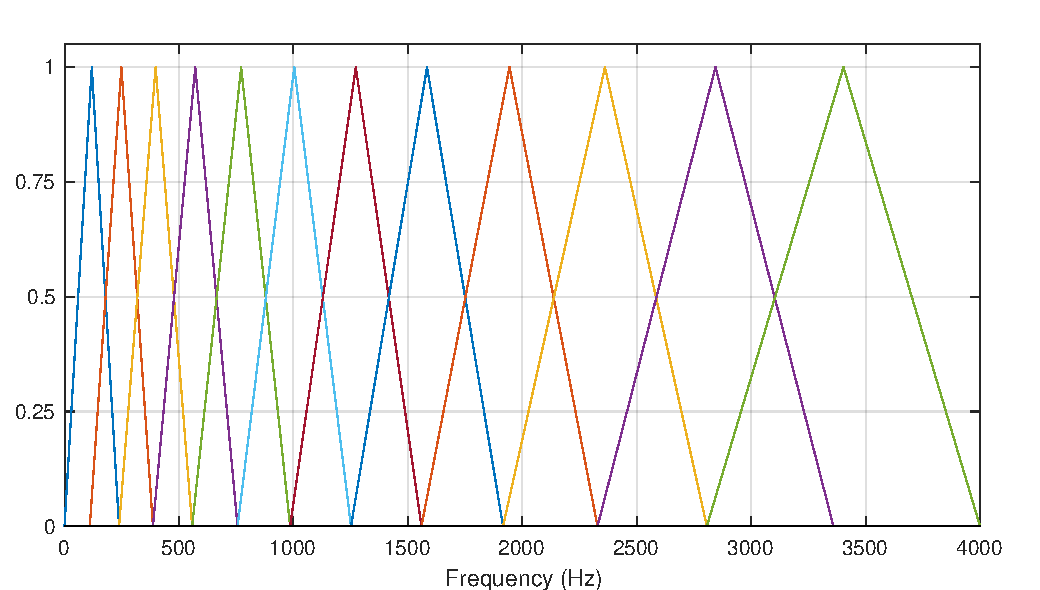
\includegraphics[trim={0cm 0cm 0cm 0.5cm}, clip, width=\textwidth]{melfilter.pdf}
	\caption{Mel-scale filter bank with 12 filter bands from 0 to 4000 Hz. Note that in practice the number of filters is typically higher, a low number of filters was used here for a clear illustration.}
	\label{fig:melbank} 
\end{figure}
In essence, the cepstrum operator deconvolves the speech signal into a linear combination of a source (excitation signal) and a filter, which can be then separated \cite[p.~306--307]{huang2001spoken}. In the \textit{source-filter} model of speech production, speech is formed by convolving a speaker-dependent excitation with a speaker-independent formant filter. We want to separate the speaker-independent filter part that corresponds to a specific phoneme \cite[p.~288--290]{huang2001spoken}. For an idealized case, this can be represented mathematically in the following way: Speech is modeled as the combination of a sound source (vocal chords) $e(n)$ and an linear acoustic filter (vocal tract) $h(n)$:
\begin{equation}
s(n) \ = \ e(n) * h(n)
\end{equation}
The Fourier transform converts convolution in the time domain into multiplication in the frequency domain:
\begin{equation}
S(k) \ = \ F\big\{ \ e(n) * h(n) \ \big\} \ = \ E(k) \cdot H(k)
\end{equation}
Through the properties of logarithms, multiplication can be separated into addition:
\begin{equation}
\log S(k) \ = \ \log \big( E(k) \cdot H(k) \big) \ = \ \log E(k) \ + \ \log H(k)
\end{equation}
A linear combination of the source and filter are then obtained with an inverse Fourier transform, which is a linear operation itself:
\begin{equation}
c(n) \ = \ F^{-1} \big\{ \log E(k) \ + \ \log H(k) \big\} \ = \ F^{-1} \big\{\log  E(k) \big\} \ + \ F^{-1} \big\{\log H(k) \big\}
\end{equation}
In practice, the separation does not work perfectly, as the source-filter model is already a simplification in itself. However, it is often an accurate enough approximation for practical usage \cite[p.~314]{huang2001spoken}. The separation can be done with linear band-pass filtering, referred to as \textit{liftering} in the cepstral domain. In practice, this can be achieved by applying a rectangular window to the cepstrum. Functionally, this is the same as simply dropping the coefficients outside the filter band. Truncating the cepstral coefficients, i.e., taking only the $n$ first coefficients, isolates the speaker-independent filter, meaning the spectral envelope displaying the formants of a speech signal. A traditional number of coefficients used is 12 \cite{huang2001spoken, gales2008application}. Conversely, the higher cepstral coefficients describe the primarily speaker-dependent excitation characteristics, corresponding to the spectral fine structure \cite{gales2008application}. The effect of cepstral truncation on the spectrum is illustrated in figure \ref{fig:cepstrum}.
\begin{figure}[h]
	\centering
	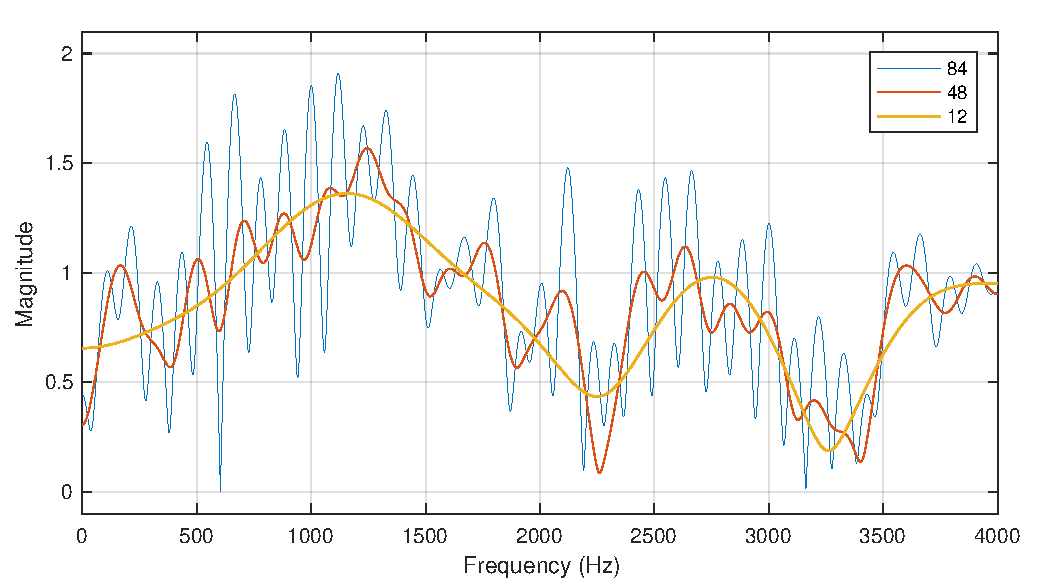
\includegraphics[trim={0.1cm 0cm 0cm 0cm}, clip, width=\textwidth]{cepstrum.pdf}
	\caption{The effect of cepstral truncation on the spectrum of a 30ms frame containing the Finnish phoneme $/a/$. The numbers describe how many cepstral coefficients are being used. As the number of coefficients is lowered, the underlying formant structure becomes clear.}
	\label{fig:cepstrum} 
\end{figure} \\
Additionally, the time varying nature of speech can be captured by taking the time derivatives of the obtained cepstral coefficients of consecutive frames \cite{gales2008application, kallasjoki2016}. The first and second-order differences, referred to as the \textit{delta} and \textit{delta-delta} features respectively, are typically used for modeling the dynamic aspects of speech. The end result is a highly condensed set of features \cite{huang2001spoken, gales2008application}. The next step in the automatic speech recognition process is to map the acoustic speech features produced into linguistic classes, that can then be used to form the actual words. This is were the \textit{acoustic model} comes in.

\subsubsection{Acoustic model}

The \textit{acoustic model} provides a statistical model for classifying feature vectors into units of speech \cite{kallasjoki2016}. One of the practical choices for these classes are the \textit{phonemes} of a particular language. Words or longer phrases could technically be used as well, however, this would lead to a very large number of classes as each word or phrase would require its own class. In written language, all words are formed with a very limited set of alphabetic letters, or \textit{graphemes}. In linguistics, a grapheme is the smallest unit of writing in any given language. For example, the English alphabet consists of 26 letters and in Finnish, 29 letters are used. Similarly, phonemes are the different units of sound that can be used to form all possible words in a particular language \cite[p.~24--25]{huang2001spoken}. For example, English is commonly divided into roughly 45 phonemes, varying slightly between different dialects and interpretations. This is very useful for acoustic modeling, since it means the acoustic model needs only to be trained to recognize this small set of phoneme classes, which can then be used to classify a practically unlimited number of different words. As the pronunciation of a phoneme depends quite heavily on the neighboring phonemes, it is common to actually use the triphone for the acoustic classes. A triphone is a sequence of three phonemes: one phoneme with the two nearest phonemes as context. Consequently, the acoustic model can be described as the collection of probabilities for how well a given feature vector corresponds to a specific phoneme sequence. \\\\
\textit{Hidden Markov Models} (HMM) have been widely used for implementing the acoustic model \cite{gales2008application, hori2013speech}. Speech is approximated well by a \textit{Markov chain}, a stochastic model for randomly changing systems where the next state depends only on the current state \cite[p.~23--26]{yu2014automatic}. The chain consists of discrete states and state changes that are modeled with transition probabilities. In a hidden Markov model, the states cannot be observed directly (hence the term \textit{hidden}). Instead, an output that is dependent on the states is known. In speech recognition, an utterance of a phoneme is considered a hidden state that emits an observable representation in the form of a feature vector. A three-state HMM is generally used to model one triphone in a left-to-right topology, meaning the states are constrained to be in chronological order \cite{kallasjoki2016}. Figure \ref{fig:hmm} present a three-state, left-to-right HMM.
\begin{figure}[h!]
	\centering
	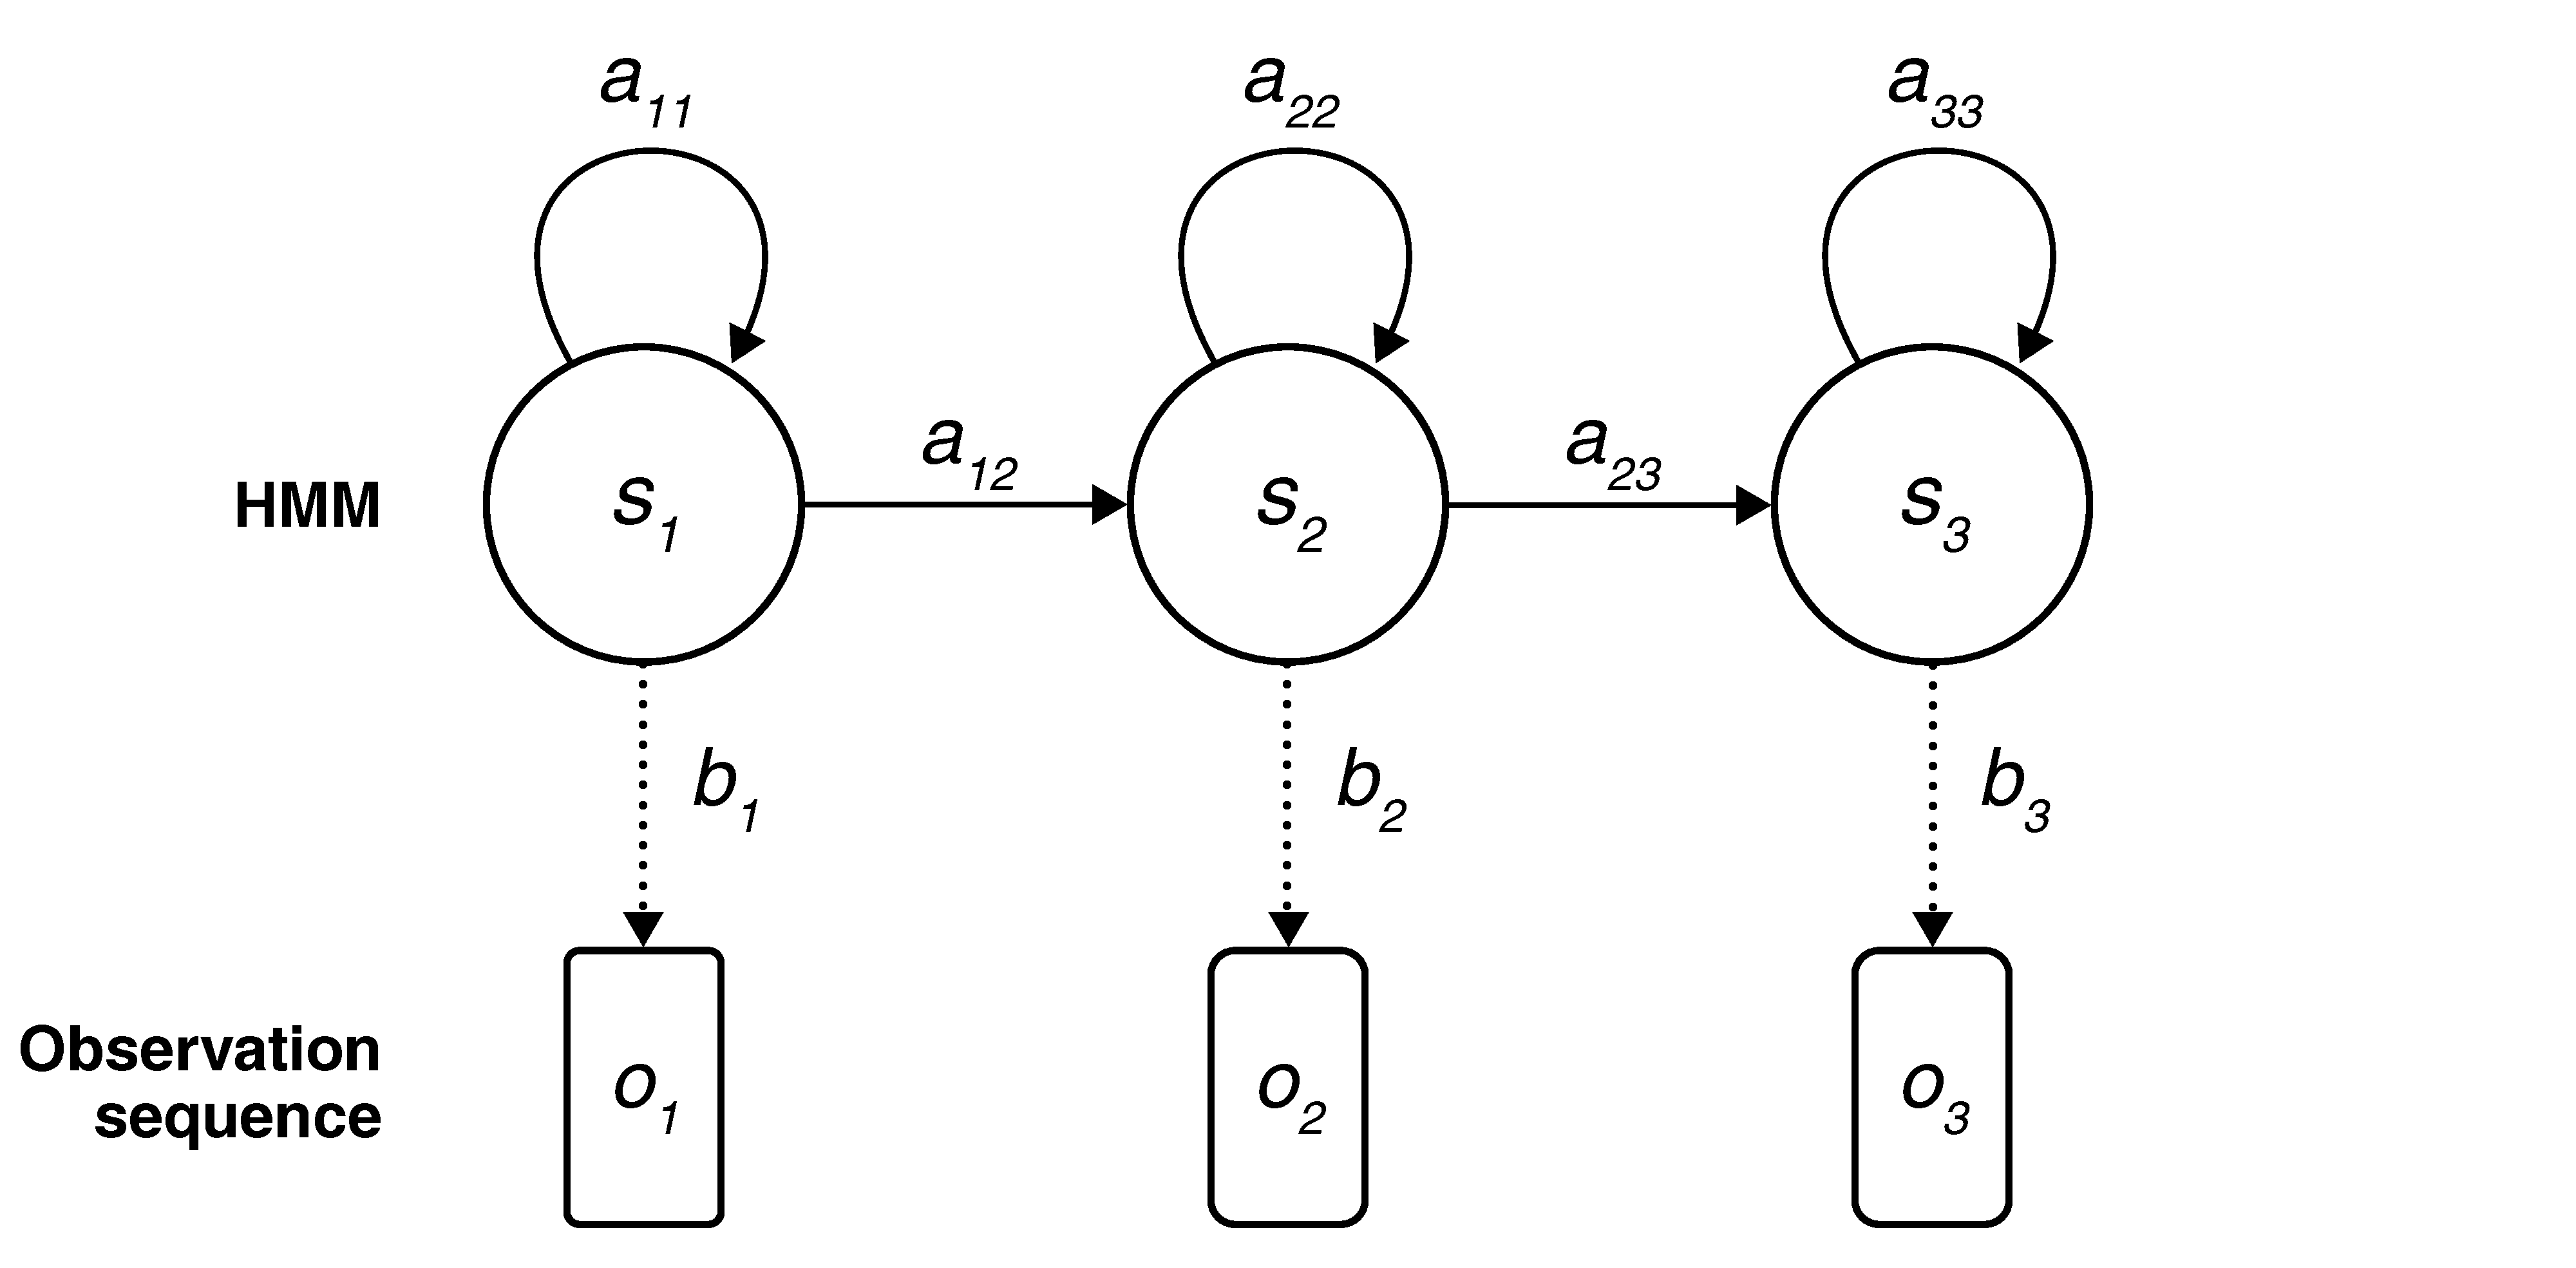
\includegraphics[width=\textwidth]{hmm.pdf}
	\caption{A three-state, left-to-right HMM diagram. $a_{ij}$ is the transition probability from state $s_i$ to state $s_j$. Each state has an emission probability distribution $b_i$ conditional over the observation sequence $O$.}
	\label{fig:hmm} 
\end{figure}
The probability that an observation is an emission of a specific state needs to be also modeled. For representing the probability distribution of observations, \textit{Gaussian Mixture Models} (GMM) have been a popular choice \cite{gales2008application, hinton2012deep}. Gaussian mixture models are built by linearly combining two or more multivariate Gaussian distributions together. A simplified example of an GMM is presented in figure \ref{fig:gmm}.
\begin{figure}[b]
	\centering
	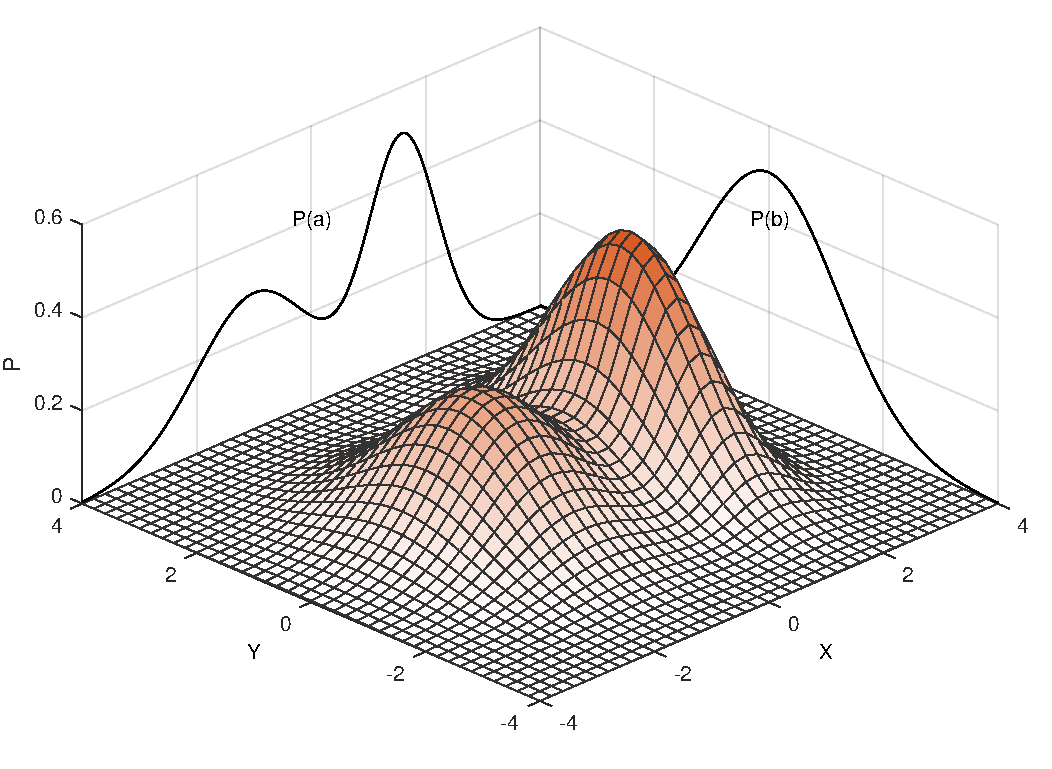
\includegraphics[trim={0cm 0.2cm 0cm 0.2cm}, clip, width=\textwidth]{gmm.pdf}
	\caption{A combination of multivariate Gaussian distributions. Note that the scaling is wrong for an actual GMM, as this is only a simple illustration. A much higher dimensionality is required as well in reality.}
	\label{fig:gmm} 
\end{figure} \\\\
Like many other aspects in ASR, GMMs have been surpassed by deep neural networks in recent years \cite{hinton2012deep}. A DNN is an artificial neural network that has two or more layers of hidden units between the inputs and outputs. DNNs are typically feed-forward, meaning data flows from the input layer to the output layer without looping back. They are trained with the \textit{backpropagation} algorithm, where the gradient of a cost function measuring the error between the desired and produced output is propagated back to the network layers \cite[p.~57--60]{yu2014automatic}. Significant improvements to speech recognition accuracy have been achieved by replacing GMMs with DNNs \cite{yu2014automatic, hinton2012deep, xiong2016achieving}. The trend of using deep neural networks for acoustic modeling has somewhat affected the way feature extraction is implemented as well, with feature extraction incorporated as one aspect of the acoustic model: The extraction process can be started with a simple linear or mel-scale spectrum, and producing the final feature representation type is relegated to the DNN, meaning the feature representation can be optimized as a part of training the acoustic model \cite{kallasjoki2016}. The ASR system used in this work is DNN based. A detailed description of the models and their training material is given in section \ref{sec:models}.

\subsubsection{Lexicon}

The \textit{lexicon} functions as a bridge between the acoustic model and the language model. It is used to describe how each word in the language model is pronounced by listing the phoneme sequence of every word. In other words, the lexicon can be defined as a dictionary for pronunciation in the context of an ASR system. Single phonemes (monophones) or triphones are normally used depending on the acoustic model. In Finnish, the pronunciation rules are very simple and each phoneme maps directly to one grapheme with only a few exceptions. Therefore, the lexicon can be generated automatically for the most part. For languages with highly irregular pronunciation rules, such as English, the lexicon is more complex and typically needs to be handcrafted by linguistic experts. Different pronunciations for the same word can also be accounted for in the lexicon. Table \ref{table:triphone} presents an example of a triphone lexicon for the same four words in Finnish as in figure \ref{fig:audio}. \\
\begin{table}[h]
	\renewcommand{\arraystretch}{1.2}  % set row height to 1.2x default
	\setlength{\tabcolsep}{20pt}       % set space between text and cell border
	\centering
	\caption{An example of a triphone pronunciation lexicon.}
	\label{table:triphone}
	\begin{tabular}{@{}ll@{}}
		\toprule
		\textbf{Word}  & \textbf{Pronunciation}              \\ \midrule
		nolla & \_--n+o \ n--o+l \ o--l+l \ l--l+a \ l--a+\_ \\
		yksi  & \_--y+k \ y--k+s \ k--s+i \ s--i+\_       	 \\
		kaksi & \_--k+a \ k--a+k \ a--k+s \ k--s+i \ s--i+\_ \\
		kolme & \_--k+o \ k--o+l \ o--l+m \ l--m+e \ m--e+\_ \\ \bottomrule
	\end{tabular}
\end{table}

\subsubsection{Language model}

The \textit{language model} contains information on how words are used to form meaningful sentences in a particular language. Instead of grammatical rules about what combinations are theoretically possible, the language model tells which words typically go together and how often they are used. Specifically, it gives the likelihood for the occurrence of a specific word sequence, which is estimated from large collections of suitable written text called a \textit{text corpus} \cite{kallasjoki2016}. Thus, the language model can be used to choose the most probable word sequence from multiple similar sounding candidates suggested by the acoustic model. Take for example the words \textit{beer} and \textit{bear}, which sound fairly similar to each other. While the sentence \textit{"one bear please"} is grammatically correct and quite possible, it is typically much more likely that \textit{"one beer please"} was spoken instead. The language model will likely assign a higher probability to the phrase \textit{"one beer please"} (depending obviously on the data it was trained with). This way, verbal context is provided for the recognition task, sorting the different hypotheses according to which are sensible and commonly used. The language model can also be used to efficiently reduce and rule-out unwanted and incorrect sentences, as word sequences with a probability of zero cannot be recognized. \\\\
Mathematically, the language model can be presented in the following way: Let $\bm{W} = w_1, w_2, w_3,\dots,w_n$ be a word sequence. The objective of the language model is to estimate the probability $P(\bm{W}) \ = \ P(w_1, w_2, w_3,\dots,w_n)$, the likelihood of that specific word sequence appearing in a particular language. Applying the chain rule of probability gives:
\begin{equation}
P(\bm{W}) \ = \ P(w_1) P(w_2|w_1) P(w_3|w_1,w_2) \dots P(w_n|w_1,\dots,w_{n-1})
\end{equation}
This means that the conditional probability $P(w_i|w_1,w_2,\dots,w_{i-1})$ must be estimated for every word $w_i$, which is generally done using \textit{maximum likelihood estimation} \cite{arisoy2008statistical}. The estimate can be calculated as the ratio of the occurrences of the word sequences $w_1,w_2,\dots,w_{i-1},w_i$ and $w_1,w_2,\dots,w_{i-1}$:
\begin{equation} \label{eq:ml}
P(w_i|w_1,w_2,\dots,w_{i-1}) \ = \ \frac{C(w_1,w_2,\dots,w_{i-1},w_i)}{C(w_1,w_2,\dots,w_{i-1})},
\end{equation}
where $C(\bm{W})$ is the frequency count of a word sequence $\bm{W}$ in a large text corpus. Due to data sparsity, this estimate has traditionally been too unreliable for long word sequences \cite{gales2008application}. As an approximation, a word $w_i$ can be assumed to depend only on a limited number of previous words. This is the \textit{n-gram model}, where the conditional probability is truncated to depend only on the $n-1$ preceding words:
\begin{equation}
P(w_i|w_1,w_2,\dots,w_{i-1}) \ \approx \ P(w_i|w_{i-n+1},\dots,w_{i-2},w_{i-1}),
\end{equation}
with $n$ ranging typically from two to four \cite[p.~210]{gales2008application}. The n-gram model has been the preferred way to construct language models for a long time \cite{gales2008application, kallasjoki2016, hirsimaki2009importance}. In practice, the n-gram probabilities estimated with equation (\ref{eq:ml}) need to be balanced, since n-grams that are present in the training material tend to get a too high probability and unseen sequences a too low probability. This process is called language model \textit{smoothing}, and can be achieved by distributing some probability mass from seen n-gram combinations to all unseen n-grams \cite{gales2008application}. \\\\
In recent years, \textit{recurrent neural networks} (RNN) have been shown to work well for language modeling \cite{enarvi2017automatic}. They differ from the feed-forward neural networks typically used in acoustic modeling in that data can flow in any direction. Due to the recurrent connections enabling arbitrarily long context information in the network, RNN language models can capture the long-term dependencies ignored by the simple n-gram model \cite{enarvi2017automatic, mansikkaniemi2017continuous}. Neural network language models overcome the data sparsity problem by projecting words into continuous space, where the probabilities are then estimated \cite{mansikkaniemi2017continuous}. While neural network language models offer improved performance for many applications, training them requires a great deal more computational resources compared to n-gram models, with the training time typically measured in days or even weeks on high-end GPUs. Memory consumption of state-of-the-art neural networks can be an issue as well on currently available GPU hardware \cite{enarvi2017automatic}. \\\\
In agglutinative languages like Finnish, Estonian, Hungarian and Turkish, words are formed primarily by concatenating suffixes to root words, as well as using compounding (i.e., joining words together) and inflections ("word bending") \cite{arisoy2008statistical, kurimo2006unlimited, hirsimaki2006unlimited}. This means that there can be millions of regularly used word forms in these languages. Therefore, it is very hard to build a word-based vocabulary that would cover all the commonly used words \cite{arisoy2008statistical}. Though it has recently become possible to build n-gram models covering millions of words, reducing the vocabulary size is important for efficient models \cite{smit17boundaries}. For English, a 60K word lexicon can be sufficient for many tasks, whereas for Finnish, even a 500K word-based lexicon would not give the same level of performance \cite{arisoy2008statistical}. The problem is the large number of \textit{out-of-vocabulary} (OOV) words when dealing with limited vocabulary sizes. \\\\
\textit{Sub-word modeling} has been successfully used to model agglutinative languages, reducing the size and complexity of the language model \cite{enarvi2017automatic, hirsimaki2006unlimited, hirsimaki2009importance, smit17boundaries}. In sub-word modeling, words are split into smaller units, which can be done based on grammatical rules or statistical techniques \cite{arisoy2008statistical}. A data-driven statistical method called the \textit{Morfessor} is commonly used for morphological segmentation. The Morfessor uses unsupervised machine learning methods to find morpheme-like statistical sub-word units called \textit{morphs}, based purely on raw text data \cite{arisoy2008statistical, kurimo2006unlimited}. A morph-based vocabulary was used in the Conversation Assistant prototype, which is described in detail in section \ref{sec:implementation}.

\subsubsection{Decoding} \label{sec:decoding}

In ASR systems, \textit{decoding} means computing the result based on the input and the statistical models, i.e., solving equation (\ref{eq:max3}), were the observation sequence $\bm{O}$ is the feature vector produced in feature extraction. The decoding process is fundamentally a search for the best matching word sequence over all possible word sequences, i.e., the \textit{search space} defined by the models \cite{pylkkonen2013towards}. However, implementing the search in practice requires efficient algorithmic solutions: The size of the search space is often huge, and grows exponentially with the number of words in an utterance \cite{pylkkonen2013towards}. Therefore, an exhaustive search over all possibilities is generally not feasible. Heuristic methods are required to limit the search space in some way. For this purpose, \textit{beam search} is commonly used \cite{pylkkonen2013towards, hori2013speech}. In beam search, only a limited number of most promising paths are kept while others are discarded in a process called \textit{pruning}. The \textit{Viterbi} dynamic programming algorithm is one such commonly used method \cite{huang2001spoken, yu2014automatic, hori2013speech}. \\\\
ASR systems are divided into \textit{online} and \textit{offline} decoders \cite{alumae2014full}. In online decoding, the input is coming continuously in real-time and speech recognition is performed concurrently with the input. In other words, speech recognition is performed in real-time and the results are typically displayed immediately. Conversely, in offline decoding the input is an existing (long) audio recording, which is then transcribed into text all at once. Offline decoding generally focuses on accuracy at the cost of speed and model size, though offline decoding can also be faster than real-time, meaning that the full transcription result is produced in less time than the length of the input file \cite{alumae2014recent}. For example, a ten minute audio file could be transcribed in five minutes. On the other contrary, online decoding sets some restrictions for the properties of the ASR system, with the primary constraint being the requirement of approximately real-time recognition. Therefore, a compromise between speed and accuracy is typically required in online recognition. For example, the size of the vocabulary may have to be limited for fast enough performance \cite{enarvi2017automatic, mcgraw2016personalized}. \\\\
The use of \textit{weighted finite state transducers} (WFST) for representing the statistical models is popular in speech recognition, especially for LVCSR systems \cite{hori2013speech, mohri2008speech, smit17boundaries}. WFSTs can be understood as a finite automaton, consisting of a set of finite states and transitions between them. Each transition has an input label, output label and a weight for the transition. They are typically used to represent and store the acoustic model, language model and lexicon in one combined transducer, which offers many practical benefits. In the WFST--based speech recognition process, the acoustic model WFST transduces an acoustic state sequence into a phoneme sequence, the lexicon WFST transduces a phoneme sequence into a word sequence, and the language model WFST transduces a word sequence into a sentence. These transducers can be integrated into a single, large WFST that directly transduces an acoustic state sequence into a sentence. The power of weighted finite state transducers for ASR comes from that they can optimize the search space and remove redundancies. The end result is a highly-optimized static structure for fast decoding, enabling real-time decoding with very large vocabularies of over one million words even on an average personal computer \cite[p.~4--6]{hori2013speech}. The ASR system used in the Conversation Assistant prototype is WFST-based.

\subsubsection{Evaluation metrics}

Measuring the performance of an ASR system is a critical part of their development, so that different systems can be compared and new algorithms or implementations evaluated \cite{huang2001spoken}. However, the answer to the question of how to measure speech recognition errors is not wholly unambiguous. It depends on what kind of occurrences in the transcription are defined as errors: For instance, are missing punctuation marks or capital letters counted as errors? In the recognized word sequence, there might be extra words added to the result or some words could be missing, in addition to the simple recognition errors were a word was transcribed incorrectly. Consequently, simply comparing two word strings one word at a time does not work: For example, if one word is missing or added as an extra, all the following words are interpreted as errors since they do not match the reference word in that position. Instead, the recognition result and the reference word string have to be aligned to each other \cite{huang2001spoken}. \\\\
Typically, the recognition errors in an ASR system are categorized as one of three main types of word errors \cite[p.~420]{huang2001spoken}:
\vspace{2mm}
\begin{itemize}[itemsep=2mm]
	\item \textbf{Substitution}: a correct word was replaced with an incorrect word.
	\item \textbf{Deletion}: a correct word was omitted.
	\item \textbf{Insertion}: an extra word was added.
\end{itemize}
\vspace{2mm}
Based on these, the \textit{word error rate} (WER) is defined as:
\begin{equation}
WER \ = \ \frac{S + D + I}{N} \cdot 100\%,
\end{equation}
where $S$ is the number of substitutions, $D$ is the number of deletions, $I$ is the number of insertions and $N$ is the total number of words in the reference text. Essentially, it is the \textit{Levenshtein distance} for words, describing the total percentage of word errors. It should be noted that it is possible for the error rate to exceed $100\%$, as the number of additions is not limited. WER is the most widely used metric for evaluating and comparing the speech recognition accuracy of ASR systems \cite{huang2001spoken, kallasjoki2016}. \\\\
For agglutinative languages such as Finnish, the WER can be a too harsh measure: Many words are formed by adding affixes to a base word, resulting in a large amount of very similar sounding words with only a slight difference in their meaning. While technically incorrect, recognition errors of one or two characters in these words will most likely not hinder the understandability as much as the WER indicates. The \textit{letter error rate} (LER) can be used as an alternative to the WER, giving a more accurate metric for agglutinative languages \cite[p.~41--42]{kallasjoki2016}. In LER, the Levenshtein distance is simply calculated for individual letters instead of full words. Other measures can be used as well, particularly for measuring very specific types of errors or special vocabulary words, such as the error rate of foreign names or acronyms \cite{mansikkaniemi2017continuous}.  \\\\
For evaluating language models, the \textit{perplexity} measure is commonly used \cite{mansikkaniemi2017continuous}. Perplexity measures how accurately a statistical model predicts a sample. In the case of the language model, this translates to how well the language model predicts a word sequence in an evaluation text sample. Perplexity is calculated by
\begin{equation}
ppl \ = \ \sqrt[N]{\prod_{i=1}^{N} \frac{1}{P(w_i|h)}},
\end{equation}
where $P(w_i|h)$ is the probability of a word sequence given by the language model and $N$ the number of words in the evaluation text. Minimizing perplexity corresponds to maximizing probability, meaning that a lower perplexity is better \cite{mansikkaniemi2017continuous}.

\subsubsection{Recognizing conversational speech}

Accurate speech recognition of everyday conversational speech has been the focus of much research in recent years, and remains challenging especially in noisy environments \cite{keronen2014approaching, kallasjoki2016, xiong2016achieving, li2014overview, keronen2010comparison, pylkkonen2013towards}. This particular area of ASR is the most relevant in the context of this work, as the Conversation Assistant is intended for use in everyday conversational situations. Conversational speech falls under the large vocabulary continuous speech recognition task, and is arguably the hardest area for online ASR. Conversational, or \textit{colloquial} speech, is typically quite informal and can differ noticeably from the standard, formal form of the language \cite{enarvi2017automatic}. In Finnish, colloquial pronunciations are also written differently than the standard word form, due to the phonetic orthography \cite{enarvi2017automatic}. Consequently, colloquial speech causes more variations to language and increases the size of the vocabulary. For agglutinative languages, a vocabulary of many million words is required in order to cover all the spelling variations in conversational speech \cite{enarvi2017automatic}. Overall, these factors have made it significantly harder to achieve a good level of speech recognition performance for conversational speech, compared to most other tasks. \\\\
Different dialects and pronunciations can pose a challenge to ASR performance, as the statistical models are only as good as the material they are trained with. Neural networks require a large amount of training data, and sourcing suitable training data covering the wide variety of distinct speaking styles can be difficult \cite{mansikka17parliament}. In order to recognize colloquial variations such as heavy accents, tens or hundreds of hours of material is typically needed for good performance. In addition, the recordings have to be accurately transcribed and aligned correctly. Even if recording are available, transcriptions are typically not, and producing them is generally expensive and time consuming \cite{mansikka17parliament}.  \\\\
Conversations are often held in acoustically challenging situations with background noise and other competing speakers. For large-scale everyday usage of ASR, noise-robustness has become an integral part for good real-world recognition performance \cite{li2014overview}. More specialized ASR tasks can be performed in a quiet environment and with special, studio-grade microphone equipment, conforming to the limitations of the ASR system. For public usage, ASR systems have to cope with all possible environments and situations instead. Likewise, external microphone setups that could noticeably improve the SNR of the input signal are an unreasonable requirement for most everyday usage. Noise-robust speech recognition remains somewhat a challenge, though a large amount of research has been done to address this issue \cite{kallasjoki2016, keronen2010comparison, keronen2014approaching, li2014overview, qian2016very}. Fundamentally, the problem arises from distortions in the transmission path of the signal from the speaker to the microphone, with the effect that the observed feature sequence does not match the utterance of the speaker \cite{kallasjoki2016, li2014overview}. These distortions can be from sources such as traffic noise, reverberation, background music, and overlapping speech. \\\\
\textit{Noise-robust} speech recognition methods attempt to reduce the mismatch between the noisy observations and the models \cite{li2014overview, kallasjoki2016, keronen2010comparison}. One straightforward way to improve speech recognition in noisy conditions is to use \textit{multi-condition training}, where the acoustic model is trained with a combination of clean and noisy data. The feature extraction process can be improved further from the standard MFCC features to be more robust against noise. Additionally, \textit{feature enhancement} methods have been presented that adaptively compensate for distortions in the features, such as using imputation methods for reconstructing missing data. Besides training noise robust models, the model parameters can adapted in real-time to the prevailing conditions \cite{kallasjoki2016}.

\subsection{Software Development} \label{subsec:soft}

This section presents a briew review of software engineering principles and software development methods. \\\\
Agile development. \\\\
User-centered design. \\\\
User interface design principles, guidelines, accessibility. \\\\
User testing. Usability testing. Test planning and organization.

\subsubsection{User-centered design}

Informal cognitive walkthroughs \cite{grigoreanu2013informal}. \\\\
Design with the deaf \cite{potter2014design}. \\\\
Unified user interface design: designing universally accessible interactions \cite{savidis2004unified}. \\\\
Influences of new media communication on the deaf/hard of hearing as reflected in interaction design \cite{chang2016}. \\\\
Evaluating alternatives for better Deaf accessibility to selected web-based multimedia \cite{shiver2015evaluating}.

\subsubsection{User testing}

In the context of this thesis, usefulness is understood as to measure how well the system fulfills and performs its intended function, which in this case translates to how much and well does the Conversation Assistant help hearing impaired persons to follow and participate in conversational situations. \\\\
Common industry format usability tests \cite{bevan1999common}. \\\\
Usability evaluation methods: Mind the gaps \cite{de2009usability}. \\\\
Group usability testing: Evolution in usability techniques \cite{downey2007group}. \\\\
A practical guide to usability testing \cite{dumas1999}. \\\\
On the contributions of different empirical data in usability testing \cite{ebling2000contributions}. \\\\
Usability testing of mobile applications: A comparison between laboratory and field testing \cite{kaikkonen2005}. \\\\
An experience in requirements prototyping with young deaf children \cite{korte2015experience}. \\\\
User-Centred Engineering \cite{richter2014user}. \\\\
Experiences with usability testing: Effects of thinking aloud and moderator presence \cite{riihiaho2015}. \\\\
Handbook of usability testing: how to plan, design and conduct effective tests \cite{rubin2008handbook}. \\\\

\subsection{Previous Work} \label{subsec:work}

Previous research and projects focusing on the same area. Previous approaches and solutions to the same problem. \\\\
Speech enhancement methods by reducing noise. \cite{goehring2016speech} \\\\
Improvements to hearing aids: The ever increasing computational power of embedded systems, and the concurrent reduction in size and power consumption... \\\\
A Personalizable Mobile Sound Detector App Design for Deaf and Hard-of-Hearing Users \cite{bragg2016personalizable}. \\\\
Innovation of a Smartphone App Design as Used in Face-To-Face Communication for the Deaf/Hard of Hearing \cite{chang2015}. \\\\
Using speech recognition technology to support education for deaf students \cite{fen2010using}. \\\\
The effects of automatic speech recognition quality on human transcription latency \cite{gaur2016effects}. \\\\
A communication aid for hearing impaired persons using mobile smart phones \cite{hirayama2011communication}. \\\\
Tablet PC and Head Mounted Display for live closed captioning in education \cite{jimenez2011tablet}. \\\\
The Exploration of the Strategies and Skills of Effective Use of Voice Recognition Software in the Classroom for Deaf Students \cite{jun2010exploration}. \\\\
Improving Real-Time Captioning Experiences for Deaf and Hard of Hearing Students \cite{kawas2016improving}. \\\\
Inclusion of deaf students in computer science classes using real-time speech transcription \cite{kheir2007inclusion}. \\\\
Tracked Speech-To-Text Display: Enhancing Accessibility and Readability of Real-Time Speech-To-Text \cite{kushalnagar2015tracked}. \\\\
Dialogue enabling speech-to-text user assistive agent with auditory perceptual beamforming for hearing-impaired \cite{lee2013dialogue}. \\\\
Scribe4Me: Evaluating a mobile sound transcription tool for the deaf \cite{matthews2006scribe4me}. \\\\
An assistive technology for hearing-impaired persons: Analysis, requirements and architecture \cite{mielke2013assistive}. \\\\
A Pilot Study about the Smartwatch as Assistive Device for Deaf People \cite{mielke2015pilot}. \\\\
Using augmented reality and automatic speech recognition techniques to help deaf and hard of hearing people \cite{mirzaei2012}. \\\\
Combining Augmented Reality and Speech Technologies to Help Deaf and Hard of Hearing People \cite{mirzaei2012combining}. \\\\
Audio-visual speech recognition techniques in augmented reality environments \cite{mirzaei2014audio}. \\\\
A mean for communication between deaf and hearing pairs in inclusive educational settings: the Sessai app \cite{prietch2015mean}. \\\\
Application Requirements for Deaf Students to use in Inclusive Classrooms \cite{prietch2015application}. \\v
Using speech recognition for real-time captioning and lecture transcription in the classroom \cite{ranchal2013using}. \\\\
Computer speech recognition as an assistive device for deaf and hard of hearing people \cite{robison1996computer}. \\\\
The application of voice recognition technology to the development and presentation of complex engineering terminology to hearing impaired students \cite{stewart2003application}. \\\\
Transcription table: text support during meetings \cite{van2005transcription}. \\\\
Audiowiz: nearly real-time audio transcriptions \cite{white2010audiowiz}. \\\\
A study and application of speech recognition technology in primary and secondary school for deaf/hard of hearing students \cite{zhili2010study}. \\

\clearpage

\section{Conversation Assistant} \label{sec:implementation}

This section describes the proposed Conversation Assistant solution and presents the detailed information on the implementation of the developed software prototype, as well as the reasoning behind the choices made. The Conversation Assistant can be best viewed as a general approach for supporting communication for deaf and hard of hearing persons, as it is not tied to only a single possible implementation method or hardware device.  

\subsection{Description}

The basic operation principle of the proposed Conversation Assistant can be described as follows: First, the speech of the speaker(s) is picked up with a microphone. This can be for example the build-in microphone of a users device, or an external microphone, preferably close to the speaker for improved signal-to-noise ratio and ASR performance. The speech input is then converted into text by an automatic speech recognition system. Finally, the recognition result is displayed on a screen for the user or users. All of these basic components can be separate from each other, or integrated into one device. The resulting text can be displayed with special visual formatting depending on additional features the system has, such as speaker recognition, enabling visual separation of speech from different speakers. \\\\
Speech recognition can be a computationally intensive task, and large models can require a lot of disk space as well as memory during operation. As such, most laptop computers can run a speech recognizer locally, but current mobile devices and less powerful computers cannot. Also, it is not practical or sensible that every user would need to download potentially multiple gigabytes of data to their own device in order for the speech recognition to happen on their device locally, even if the computational resources were sufficient. Instead, a server-based solution is needed, where the audio signal is acquired at the end-device and is then send via the internet to a server handling the speech recognition process. The server then simply returns the recognition results as a text string to the device for display. This is the way most ASR systems aimed for general consumers currently work already. The major downside of the server-based implementation is the required internet connection. \\\\
Mobile devices \cite{mcgraw2016personalized}.

\subsection{Implementation}

Finnish ASR.

\subsubsection{Kaldi ASR toolkit}

\href{http://kaldi-asr.org/doc/index.html}{Kaldi} is an open-source speech recognition toolkit, intended primarily for speech recognition research. Kaldi is written in C++ and licensed under the Apache License v2.0. \cite{kaldi} \\\\
GStreamer plugin around Kaldi's online neural network decoder \cite{alumae2014full}. Server-based version \cite{alumae2012open}. \\\\

\subsubsection{Models} \label{sec:models}

Acoustic model = speecon data: headset, lapel \& kaukomikit (1m), julkinen paikka ja auto. \cite[p.~43]{kallasjoki2016}. Kallasjoki, Remes, Keronen jne paperit. \\\\
Language model:  kielipankki, euroopan parlamentin käännetyt tekstit. \\\\
Morph-based vocabulary. \\\\
nnet2-online i-vector hr mfcc. \\\\
i-vector speaker adaptation \cite{xiong2016achieving, kaldi}.


\subsubsection{GUI}

Python. GTK. PyGST. The source code for the prototype is included in appendix \ref{sec:proto}.

\clearpage

\section{User Testing} \label{sec:testing}

User testing was used to validate the Conversation Assistant approach for helping with the conversational challenges faced by hearing impaired persons, and to examine how well the prototype succeeds in this, as well as to find out the key areas for improvement. Additionally, the user tests were used to gauge the interest of potential end-users towards this type of assistive approach and its commercial potential. Through user testing, it was also possible to collect valuable feedback and opinions from real end-users on for example what kind of features would they want to have, and in what kind of situations would they use the Conversation Assistant. With the information learned from user testing, it is possible to develop the Conversation Assistant to better fulfill the needs of the target audience, making it more helpful to them. Not only will this help hearing impaired people lead better lives, but can also increase the commercial potential of this type of assistive application. More commercial potential will in turn increase the likelihood that applications actually become available to the general public and in many different languages.

\subsection{Objectives}

The primary goal of the user testing was to determine if the Conversation Assistant is in fact helpful, and to assess how useful it is in the opinion of intended end-users. The secondary goal was to identify which factors contribute the most towards increased usefulness for the end-users. The reasoning behind this secondary objective was that while it is easy to identify many technical aspects that could be improved, like for example the speed of the speech recognizer, it might not actually matter for the end-users. If for example the users feel that on average, the speech recognition accuracy is already good enough, then improving it further would not probably increase the experienced usefulness very much. Therefore, the user tests were designed to focus more on qualitative properties as experienced by the users, instead of quantitative, objective measurements for the performance of the Conversation Assistant. It is also a lot harder to measure meaningful objective data of users interacting with devices and software, than it is to get their subjective opinion on the matter. \\\\
Ultimately, it is the subjective experience of the end users that matters when evaluating the validity and usefulness of the Conversation Assistant. In fact, typical objective measurements like the word error rate (WER) of the speech recognizer might not actually be the most relevant for this specific application \cite{wang2003word}. A better WER does not automatically mean that the quality of the recognition result is also better in terms of understanding the contents. Also, the end-goal of the Conversation Assistant is not to have perfect transcriptions of speech, but to support and supplement the users hearing in real-time conversational situations. If the user can understand everything spoken to them with the help of the system, even though the text is full of errors, then it is succeeding in its intended purpose regardless of the speech recognition accuracy. Research indicates that in real-time situations the type of errors is much more important than simply the overall percentage when it comes to understandability and helpfulness \textbf{[V!]}. This observation feels inherently logical for conversations: It is easy to imagine that a few extra letters or words, or a slightly wrong grammatical case might not affect the understandability of a sentence considerably, whereas a missing key word might render the transcript almost useless. In conversational situations between humans, a lot of information can be interpreted based on the context and other factors like non-verbal cues (\textbf{V!}). This was reported also by our test users, saying that in many cases they could guess the meaning of a sentence well enough from incomplete and erroneous transcripts. Based on these observations, it could be more meaningful to quantify what kind of errors the speech recognizer makes, and more importantly, how each type of error affects the usefulness of the Conversation Assistant. \\

\subsection{Design}

Now that the objectives are defined and the questions to which answers are wanted to are known, the question becomes how to actually answer those questions: What tests should be performed, and how should they be performed in order for the results to be valid and as accurate as possible. The latter part is especially important when the tests involve humans, as there are many complex factors involved that could introduce bias or otherwise distort the results if the tests are not designed and executed properly. There are also ethical matters and privacy concerns to consider whenever human test subjects are involved. \cite{rubin2008handbook} \\\\
Potential objective measurements considered included eye-tracking, which could have been used to accurately determine the percentage of time the users spend watching the Conversation Assistant screen instead of the person speaking. Eye-tracking could also be used to assess how people tend to use the Conversation Assistant: Do they look back-and-forth quickly between the speaker and the screen, or do they first try to listen a full sentence watching the speaker, and only after that check the screen for help. The User Interfaces research group at Aalto has experience in eye-tracking and could have provided the necessary equipment if desired. While this information would be interesting from a HCI point-of-view, and have some implications for the UI design and recognition result displaying, it does not answer significantly to the primary and secondary objectives set out for the tests at this stage. It is also possible to obtain a decent approximation for this data by analysing the video recording of the test session, which can also show were the test subject was looking at on any given moment during the test. To avoid manually gathering this data from the video, computer vision methods for eye-tracking could be used to get quite accurate results automatically. For example, Krafka et al. used deep convolutional neural networks for successfully tracking eye movement on mobile device cameras \cite{krafka2016eye}. \\\\  
Using recordings for a consistent, standardized source of speech. Missing the human element and non-verbal cues. Wanted to test in real situations.

\subsection{Test plan}

The final test design consisted of two separate test sections and was designed to take approximately one hour in total. One hour was chosen as it represented a good balance between the test subject getting a thorough experience without test fatigue setting in. It was also a practical choice as it made scheduling the test sessions easy. Each section had first a short practice run without using the Conversation Assistant. This was done to familiarize the test subject with the task and to give them a baseline reference for their ability to understand speech, in order for them to then be able to better estimate the usefulness of the Conversation Assistant. The first test section was designed to be a passive situation for the test subject, where the test subject is only listening to speech. The second section was an active interaction situation, where the test subject is speaking and listening in equal parts. The full test routine with the schedule is presented below, followed by a detailed description of each section: \\
\begin{enumerate}[font=\bfseries]
	\item \textbf{Introduction} (10 min)
	\begin{enumerate}[label*=\arabic*.]
		\item Research overview
		\item Legal documents
		\item Instructions
		\item Background information questionnaire
	\end{enumerate}
	\item \textbf{Section 1: Word explaining} (20 min)
	\begin{enumerate}[label*=\arabic*.]
		\item Without the Conversation Assistant (5 min)
		\item With the Conversation Assistant (10 min)
		\item Questionnaire (5 min)
	\end{enumerate}
	\item \textbf{Section 2: Conversation} (20 min)
	\begin{enumerate}[label*=\arabic*.]
		\item Without the Conversation Assistant (5 min)
		\item With the Conversation Assistant (10 min)
		\item Questionnaire (5 min)
	\end{enumerate}
	\item \textbf{Debriefing} (10 min)
	\begin{enumerate}[label*=\arabic*.]
		\item Questionnaire (5 min)
		\item Reward \\
	\end{enumerate}
\end{enumerate}

\subsubsection{Introduction}

The user test session started with an introduction section to gently prepare the test subject for the test situation, as is the recommended standard procedure in user and usability testing \cite{dumas1999, rubin2008handbook}. To begin with, the research topic and purpose of the test is explained to the participant together with their role in it. After the general orientation, the person is asked to fill the required legal documents, which in this case consisted of the typical research consent form as well as a permission to record and use the audiovisual recordings made during the session. Then the subject was presented with the test routine and schedule for the session, and more detailed instructions for their task in each section. All of the above mentioned materials were provided in written form to ensure that everything is understood regardless of the subjects level of hearing loss. Finally, the test subject was asked if they have any questions about the test or their task, and the test proceeded forward to the last part of the introduction after the subject indicated that all was clear. \\\\
At the end of the introduction section, the test subject was asked to fill the first page of the test questionnaire, which was used to gather some basic background information on the person, as well as their previous experience with automatic speech recognition technology and mobile devices. These questions included the subjects age, their current employment status (student, employed, unemployed, retired), hearing aids and other assistive devices they use, and whether they own a smartphone and/or a tablet. This information can be useful in analyzing and understanding the results, if for example the subjects age or self-professed skill with computers affected the perceived usefulness and ease of use of the Conversation Assistant.

\subsubsection{Section 1: Word explaining}

Section one consisted of a word explaining exercise, where the test subjects tries to deduce the word under question based on the explanation of the test administer. The words were kept fairly simple as the intention was only to confirm that the test subject had understood what had been said, not to test the deduction skills and general knowledge of the person. The word list used contained a little over 30 words, of which approximately ten were used for the first try without the Conversation Assistant, and the rest with the Conversation Assistant. The same words were used for all test subject, though not in the same exact order, to minimize their effect on the results. Section one would conclude when there was no more words left, or if the time allocated was exceeded by more than a few minutes. After the test, the test subject was asked to fill a questionnaire related to the section, asking the person's opinion on the performance of the Conversation Assistant in that particular section.

\subsubsection{Section 2: Conversation}

Section two was a bilateral conversation situation, which closely resembled a typical free conversation between two persons. The test administer had a list of simple conversation topics that anybody should be able to talk about comfortably, like food, traveling, entertainment, and hobbies. The topics were presented in the form of a question, like for example "what are your favorite foods?" or "what would you do if you won the lottery?". To initiate the conversation, the test administer would start with a question like this, and then wait for the test subject to answer it, before answering himself. Then, the test administer would keep the conversation going by asking follow-up questions and continuing to discuss the topic. After a topic was exhausted, the test administer would move on to the next topic and start the cycle of questions again. One topic was done without the Conversation assistant, and there rest with it. As before, there was a questionnaire in the end.

\subsubsection{Debriefing}

After both test sections, the test subject was asked to fill one last questionnaire about the Conversation Assistants overall usefulness. The post-test questionnaire also contained broader questions about this type of assistive application in general, like "in what situations would you use the Conversation Assistant?", as well as how much would they be willing to pay for it. The session ended with filling the financial forms for paying the reward.

\subsection{Questionnaire} \label{sec:quest}

Questionnaire design principles. \cite{dumas1999}. Unbiased questions. \\\\
A linear scale with discrete steps from one to seven was used for the numerical questions. Other question types included questions with binary yes or no answers, multiple choice questions, and written-answer questions. Each numerical question also had a text field for optional written comments, excluding some of the background questions as well as question with a written answer already. \\\\
The questionnaire was implemented with \href{https://www.google.com/forms/about/}{Google Forms}, an online tool for creating for creating surveys and questionnaires. Using a web-based interactive questionnaire instead of a printed paper version had numerous benefits in addition to being fast and simple to implement: it is easy to control that all required questions are answered, and more importantly, that each type of question is answered in the correct way. For example in multiple-choice question, only one option can be picked in the web widged as was intended. Best of all, all the numerical data and text is acquired directly in digital format, formatted appropriately in a spreadsheet without the need to manually transcribe the data from a paper. Not only does this save a significant amount of time, but it also ensures that there aren't any errors in the collected data due to human transcription errors. Transcribing hand-written text can be especially problematic due to ambiguous or unreadable handwriting. \\\\
The questionnaire was originally made and administered in Finnish, as that was the language used in the Conversation Assistant prototype and also the native language of the test subjects. It has been translated here to English as accurately as possible, but there are some small differences in the exact wording of the questions. A translation of the test questionnaire is presented below, and the actual questionnaire used in the test sessions is included in appendix \ref{sec:kysely}. \vspace{0.15cm}  \\

% make a custom enumerate list for the questionnaire
\newlist{questionnaire}{enumerate}{4}
\setlist[questionnaire]{label=\textbf{\arabic*.}, leftmargin=1.1cm, labelsep=-0.2cm, align=left, itemsep=2mm}
% settings for tasks 
\settasks{
	label-align 	    = left,
	label-width        = 0em,
	label-offset       = 0em,
	item-indent       = 0em,
	column-sep       = -4em,
	item-format       = \textit,
	counter-format = (tsk[a]),
	debug 		         = false
}
{ \footnotesize % smaller font for whole list
	\noindent
	\hspace{0.35cm}
	\textbf{Background information}
	\vspace{0.15cm} 
	\begin{questionnaire}
		\item Name?
		\item Email?
		\item Age?
		\item Occupation?
		\begin{tasks}[label-width = 2em](4)
			\task student
			\task employed
			\task unemployed
			\task retired
		\end{tasks}
		\item Do you own a smartphone?
		\begin{tasks}[label-width = 2em](2)
			\task yes
			\task no
		\end{tasks}
		\item Do you own a tablet?
		\begin{tasks}[label-width = 2em](2)
			\task yes
			\task no
		\end{tasks}
		\item Do you use a hearing aid or other assistive devices for hearing? If yes, please specify what.
		\item Have you previously used an application or service that uses automatic speech recognition?
		\begin{tasks}[label-width = 2em](2)
			\task yes
			\task no
		\end{tasks}
		\item If you answered \textit{yes} to question 8, please specify what applications and services?
		\item In your own opinion, how proficient are you at using computers and mobile devices in everyday life?
		\begin{tasks}[](10)
			\task*(2)[] bad
			\task[] 1
			\task[] 2
			\task[] 3
			\task[] 4
			\task[] 5
			\task[] 6
			\task[] 7
			\task[] good \\\\
		\end{tasks}
	\end{questionnaire}
	\noindent
	\hspace{0.35cm} \textbf{Section 1}	
	\begin{questionnaire}[resume]
		\item Did the Conversation Assistant help you to understand speech?
		\begin{tasks}[](10)
			\task*(2)[] not at all
			\task[] 1
			\task[] 2
			\task[] 3
			\task[] 4
			\task[] 5
			\task[] 6
			\task[] 7
			\task[] very much
		\end{tasks}
		\item Was using the Conversation Assistant easy?
		\begin{tasks}[](10)
			\task*(2)[] not at all
			\task[] 1
			\task[] 2
			\task[] 3
			\task[] 4
			\task[] 5
			\task[] 6
			\task[] 7
			\task[] very easy
		\end{tasks}
		\item Did using the Conversation Assistant make it harder to follow speech?
		\begin{tasks}[](10)
			\task*(2)[] not at all
			\task[] 1
			\task[] 2
			\task[] 3
			\task[] 4
			\task[] 5
			\task[] 6
			\task[] 7
			\task[] very much
		\end{tasks}
		\item Was the speech recognition fast enough?
		\begin{tasks}[](10)
			\task*(2)[] too slow
			\task[] 1
			\task[] 2
			\task[] 3
			\task[] 4
			\task[] 5
			\task[] 6
			\task[] 7
			\task[] fast enough
		\end{tasks}
		\item Were the speech recognition results accurate enough (speech was recognized correctly)?
		\begin{tasks}[](10)
			\task*(2)[] unusable
			\task[] 1
			\task[] 2
			\task[] 3
			\task[] 4
			\task[] 5
			\task[] 6
			\task[] 7
			\task[] good enough \\\\
		\end{tasks}
	\end{questionnaire}
	\noindent
	\hspace{0.35cm}
	\textbf{Section 2}	
	\vspace{0.15cm} 
	\begin{questionnaire}[resume]
		\item Did the Conversation Assistant help you to understand speech?
		\begin{tasks}[](10)
			\task*(2)[] not at all
			\task[] 1
			\task[] 2
			\task[] 3
			\task[] 4
			\task[] 5
			\task[] 6
			\task[] 7
			\task[] very much
		\end{tasks}
		\item Was using the Conversation Assistant easy?
		\begin{tasks}[](10)
			\task*(2)[] not at all
			\task[] 1
			\task[] 2
			\task[] 3
			\task[] 4
			\task[] 5
			\task[] 6
			\task[] 7
			\task[] very easy
		\end{tasks}
		\item Did using the Conversation Assistant make it harder to follow speech?
		\begin{tasks}[](10)
			\task*(2)[] not at all
			\task[] 1
			\task[] 2
			\task[] 3
			\task[] 4
			\task[] 5
			\task[] 6
			\task[] 7
			\task[] very much
		\end{tasks}
		\item Did using the Conversation Assistant slow down the conversation?
		\begin{tasks}[](10)
			\task*(2)[] not at all
			\task[] 1
			\task[] 2
			\task[] 3
			\task[] 4
			\task[] 5
			\task[] 6
			\task[] 7
			\task[] very much
		\end{tasks}
		\item Was the speech recognition fast enough?
		\begin{tasks}[](10)
			\task*(2)[] too slow
			\task[] 1
			\task[] 2
			\task[] 3
			\task[] 4
			\task[] 5
			\task[] 6
			\task[] 7
			\task[] fast enough
		\end{tasks}
		\item Were the speech recognition results accurate enough (speech was recognized correctly)?
		\begin{tasks}[](10)
			\task*(2)[] unusable
			\task[] 1
			\task[] 2
			\task[] 3
			\task[] 4
			\task[] 5
			\task[] 6
			\task[] 7
			\task[] good enough \\\\
		\end{tasks}
	\end{questionnaire}
	\noindent
	\hspace{0.35cm}
	\textbf{Debriefing}
	\vspace{0.15cm} 
	\begin{questionnaire}[resume]
		\item Was the Conversation Assistant useful in the test situations?
		\begin{tasks}[](10)
			\task*(2)[] not at all
			\task[] 1
			\task[] 2
			\task[] 3
			\task[] 4
			\task[] 5
			\task[] 6
			\task[] 7
			\task[] very much
		\end{tasks}
		\item Do you consider it to be important that the size and color of the font can be freely adjusted?
		\begin{tasks}[](10)
			\task*(2)[] not at all
			\task[] 1
			\task[] 2
			\task[] 3
			\task[] 4
			\task[] 5
			\task[] 6
			\task[] 7
			\task[] very important
		\end{tasks}
		\item Did using the Conversation Assistant make it harder to follow speech?
		\item What was good about the Conversation Assistant?
		\item What needs to be improved in the Conversation Assistant?
		\item What features would you like to have in the Conversation Assistant?
		\item Would you use, or have you already used an application like the Conversation Assistant?
		\item In what situations would you use the Conversation Assistant?
		\item How much would you be ready to pay monthly for an application like the Conversation Assistant?
		\begin{tasks}[label-width = 2em](6)
			\task 0€
			\task 1-5€
			\task 5-10€
			\task 10-20€
			\task 20-30€
			\task more than 30€
		\end{tasks}
		\item How much would you be ready to pay as a single payment for an application like the Conversation Assistant?
		\begin{tasks}[label-width = 2em](6)
			\task 0€
			\task 1-5€
			\task 5-10€
			\task 10-20€
			\task 20-30€
			\task more than 30€
		\end{tasks}
		\item Would you rather pay a monthly fee or a single payment for an application like the Conversation Assistant?
		\begin{tasks}[label-width = 2em](2)
			\task Single payment
			\task Monthly fee \\\\
		\end{tasks}
	\end{questionnaire}
}

\subsection{Execution}

The testing sessions were conducted at the Aalto university Acoustics Laboratory listening room, which is designed to conform to the strict room acoustic requirements set in the International Telecommunication Union recommendation ITU-R BS.1116 for performing critical listening tests \cite{ITU1116, jarvinen1999kuunteluhuone}. The dimensions of the room are $6,25$ and $5,6$ meters, for an area of $35$ square-meters. The test setup consisted of a small table in the middle of the room with two chairs facing each other on opposing sides of the table. One chair was for the test subject and the other for the person administering the test. A Lenovo ThinkPad T460p 14" laptop running the Conversation Assistant application was placed on the table in front of the test subject. For audio input, the test administer had a DPA 4061 miniature microphone as a lapel microphone, connected to the laptop through a Focusrite Scarlett 2i4 USB audio interface. The purpose of the microphone was to capture the speech of the test administer, i.e., the person who the Conversation Assistant user (test subject) is conversing with. The speech of the application user (test subject) was not intended to be captured or translated to text, though some of it was nevertheless picked up by the microphone. The loudspeaker configuration in the listening room consists of nine \href{https://www.genelec.com/}{Genelec} 8260A active loudspeakers positioned evenly on a circle, at ear-level when sitting on a chair. The chair of the test subject was positioned to be approximately in the middle of the loudspeaker circle for optimal audio reproduction. The need for loudspeakers is explained in detail in the next section. The test session was recorded using a Panasonic video camera with a RØDE on-camera stereo microphone facing the test subject. The full test setup layout is presented in figure \ref{fig:setup}, and a photograph from the real situation is shown in figure \ref{fig:photo}. \\
\begin{figure}[h]
	\centering
	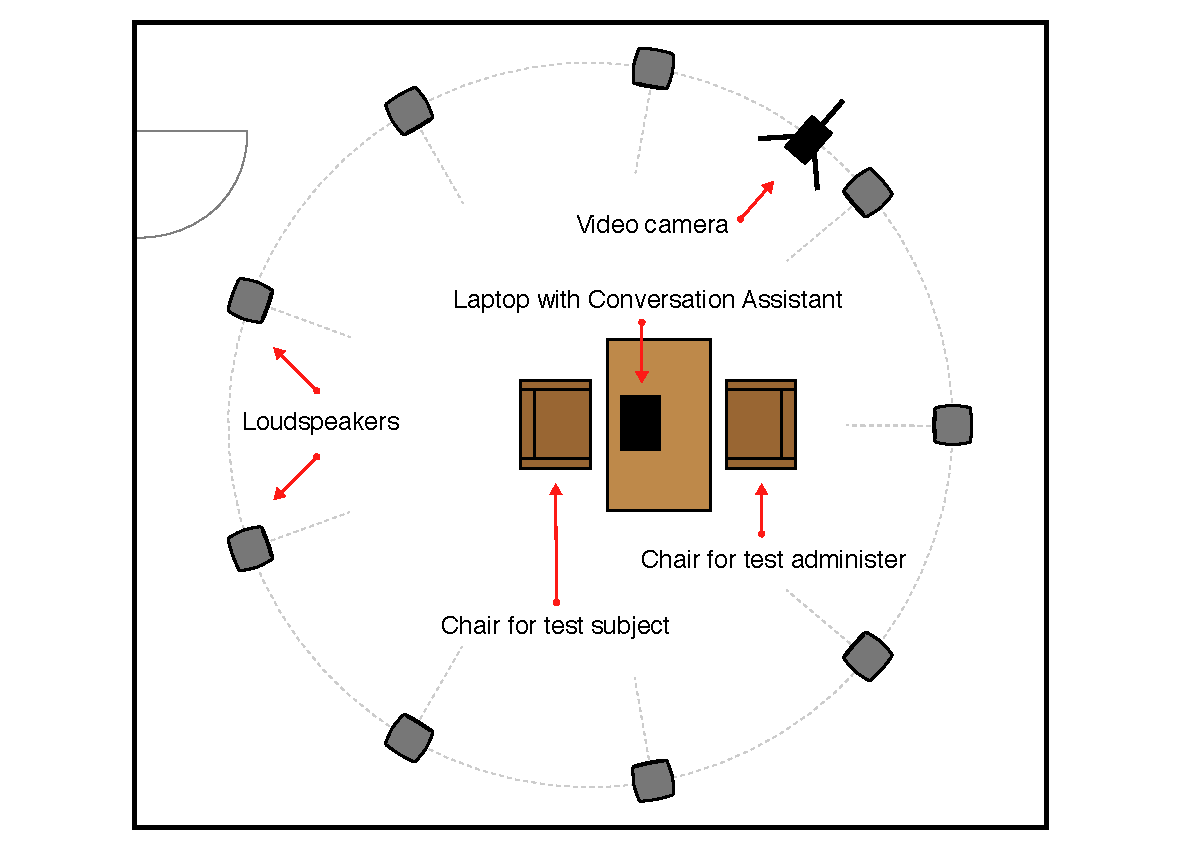
\includegraphics[trim={2cm 0cm 2cm 0cm}, clip, width=\textwidth]{setup2.pdf}
	\caption{User test setup in the listening room.}
	\label{fig:setup} 
\end{figure}
\begin{figure}[h]
	\centering
	\includegraphics[width=\textwidth]{test.jpg}
	\caption{A photo of the test environment.}
	\label{fig:photo}
\end{figure}

\subsubsection{Background noise simulation}

In order for the user test situation to better reflect the actual environments and situations where the Conversation Assistant would be typically used, background noise recordings were utilized to simulate a more realistic setting. Background noise is one of the critical factors for the whole Conversation Assistant process in two ways: Firstly, noise directly affects how well people can hear and understand speech \cite{pulkki2015communication}, and secondly, noise can drastically affect the accuracy of automatic speech recognition \cite{kallasjoki2016}. Furthermore, the impact of noise on speech intelligibility is generally even more pronounced for hearing impaired persons \cite{healy2016difficulty}, which was also reported by our test subjects. \\\\
The low background noise level and distinct acoustic properties of the listening room, namely, a short reverberation time of 0,3 seconds, offer a very idealized environment for both listening to speech and automatic recognition of speech. As such, the results obtained without added background noise would in all likelihood apply poorly to actual real-life usage. During the user tests, background noise recordings proved to be essential for successful testing, as many of the test subjects could hear and understand speech remarkably well with the help of modern hearing aids and cochlear implants, even though they were clinically categorized as having severe hearing loss or deafness. The background noise level was set to a predefined level at the beginning of each test section, approximately matching the sound pressure level measured at the recording location. The level was adjusted during the test session if needed, in cases where the test subject felt that they could hear too well, meaning that they didn't need to rely on the Conversation Assistant at all in order to follow the conversation. \\\\
The multi-channel audio listening setup installed in the listening room, combined with surround sound recordings in B-format enabled us to accurately and realistically reproduce the surround sound field present at the recording locations. B-format surround recordings are captured using a coincident microphone array, which produces four microphone signals: one omnidirectional ($W$), and three figure-of-eight channels on an orthogonal axis ($X,Y,Z$). These four signals describe the full-sphere sound field at the location of the microphone array, and can be decoded for playback on an arbitrary loudspeaker configuration (though a minimum of four loudspeakers are needed for reproducing the horizontal plane and at least six for full-sphere sound). \cite[p.~287--290]{furness1990ambisonics, pulkki2015communication} \\\\
The Aalto Spatial Sound research group provided us with their previously made background noise recordings of public places, recorded using a \href{http://www.soundfield.com/}{SoundField} ST350 portable surround microphone. Each of the two sections of the user test had their own noise environment. The first background is a city street containing mostly traffic noise, recorded near the Havis Amanda statue at the Helsinki Market Square (Kauppatori). The second is a busy cafe located on the Boulevard (Bulevardi) street in Helsinki, containing clamor and noise typical for busy cafes with poor acoustics, as well as some quiet background music. These two environments were selected because they represent locations were conversations often take place, the type of noise is challenging to both humans and automatic speech recognition, and the recordings were consistent in sound and level. Other recordings that could have been chosen included the inside of a moving bus and a regional train. \\\\ 
The Directional Audio Coding (DirAC) method developed at the Aalto University Acoustics Lab was used to decode the B-format recordings for the nine-channel speaker configuration used. The DirAC decoder divides the B-format audio input into frequency bands using the Equivalent Rectangular Bandwidth (ERB) psychoacoustic frequency scale. For each frequency band, the B-format audio is then divided into single-channel audio channels for each loudspeaker using virtual cardioid microphones based on the loudspeaker configuration information given to the decoder. Directional and diffuseness analysis is performed for each band and used to adjust the gain and diffusion parameters of each loudspeaker channel within the frequency band. Each loudspeaker signal is then the sum of all frequency bands. \cite[p.~291--292]{pulkki2006directional, pulkki2015communication} \\\\
Using DirAC, the recordings were rendered into nine-channel uncompressed PCM audio files (.wav) for easy playback. Only the horizontal sound plane was used, as it was deemed to be enough for the purpose of the user tests. Both audio scenes had multiple recordings of around one minute in length on average, made successively in the same location. For the tests, a constant background noise playing continuously during each test section was needed. Therefore, each pre-rendered nine-channel recording was split into separate mono files for each channel using \href{https://se.mathworks.com/products/matlab.html}{MATLAB}. Then the clips from each channel were edited together to form a longer loop in an audio editing software, and finally combined back to a nine-channel file in MATLAB. The \href{https://cycling74.com/products/max/}{Max/MSP} visual programming language was used to play the resulting nine-channel PCM audio loops. The Max patch consists of a simple GUI for loading the audio file, controlling playback and adjusting the volume, which is presented in figure \ref{fig:max}. \\
\begin{figure}[h]
	\centering
	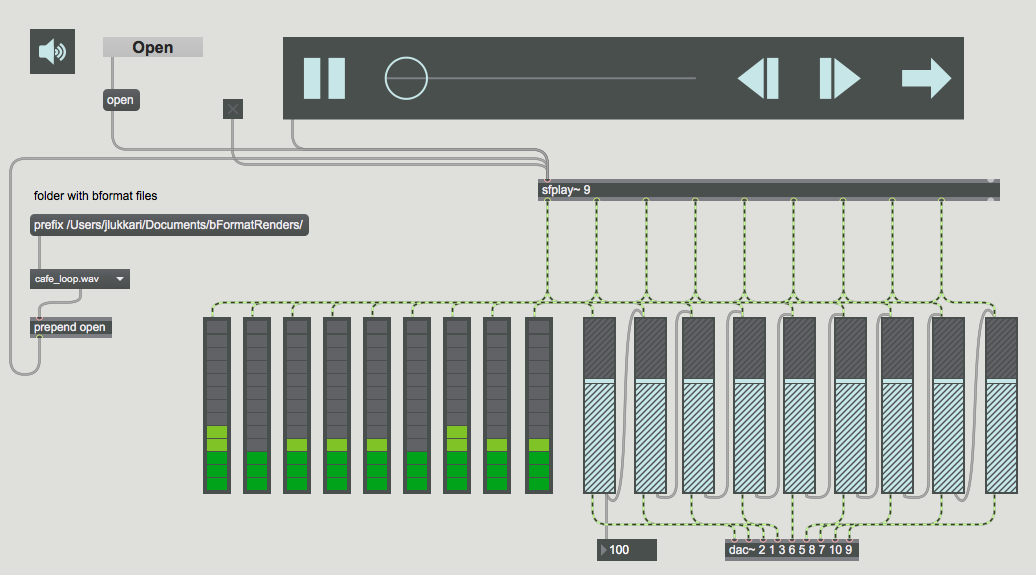
\includegraphics[width=\textwidth]{max.png}
	\caption{Max/MSP patch for playing nine-channel audio files.}
	\label{fig:max} 
\end{figure}

\subsubsection{Test participants}

The plan was for 10-12 test participants. After the preliminary filtering, we had ten suitable persons who were able to participate in the test during the days and times suitable for us. One participant had an accident that resulted in a minor injury, forcing her to cancel a few days before the scheduled test session. Unfortunately, we were not able to reschedule a new time, and as a consequence ended up with only nine test subjects in total. The relevant basic information about the test subjects is presented in table \ref{table:testsubjects}. There were eight females and one male test subject, ranging from the age of 15 to 74. Two of the test subjects did not report their age, but were estimated to be between 60 and 70 years old. The average age for the seven persons who reported it was 44 years, moving closer to 50 years when including the estimated age for the two others. The test participant group included one student, two retirees, and six employed persons. Two of the participants did not use any major assistive devices (cochlear implant or hearing aid), and were completely deaf. They could however speak and answer questions verbally. Three of the participants had cochlear implants, one in both ears and two in one ear. One of these two used a hearing aid in the other ear in addition to a cochlear implant. Four persons relied on a hearing aid, three in one ear and one in both ears.

\begin{table}[]
	\renewcommand{\arraystretch}{1.2}  % set row height to 1.2x default
	\setlength{\tabcolsep}{9pt}                % set space between text and cell border
	\centering
	\caption{Test participants.}
	\label{table:testsubjects}
	\begin{tabular}{@{}lcll@{}}
		\toprule
		\textbf{Sex} & \textbf{Age} & \textbf{Status} & \textbf{Assistive devices}                          \\ \midrule
		female       & -            & retired         & hearing aids in both ears                           \\ \midrule
		female       & -            & employed        & none                                                \\ \midrule
		female       & 15           & student         & cochlear implants in both ears, FM system in school \\ \midrule
		female       & 36           & employed        & none                                                \\ \midrule
		female       & 38           & employed        & hearing aid in one ear                              \\ \midrule
		female       & 40           & employed        & cochlear implant, induction loop                    \\ \midrule
		female       & 50           & employed        & hearing aid, induction loop, FM system              \\ \midrule
		female       & 56           & employed        & hearing aid in one ear, FM system                   \\ \midrule
		male         & 74           & retired         & cochlear implant, hearing aid                       \\ \bottomrule
	\end{tabular}
\end{table}

\clearpage

\section{Results} \label{sec:results}

In this section, the results obtained from the Conversation Assistant user testing are presented and analyzed. In the user testing, we focused on obtaining the subjective opinions of the intended end-users on the overall usefulness of the Conversation Assistant, as well as gathering user feedback on the key areas still in need of improvement. By design, our user testing produced qualitative data. MATLAB was used for analyzing the test data, as well as producing all figures. \\\\
Answers to questions with a \textit{yes or no} answer are visualized in figure \ref{fig:results_pie}. 
\begin{figure}[b]
	\centering
	\begin{subfigure}[b]{0.45\textwidth}
		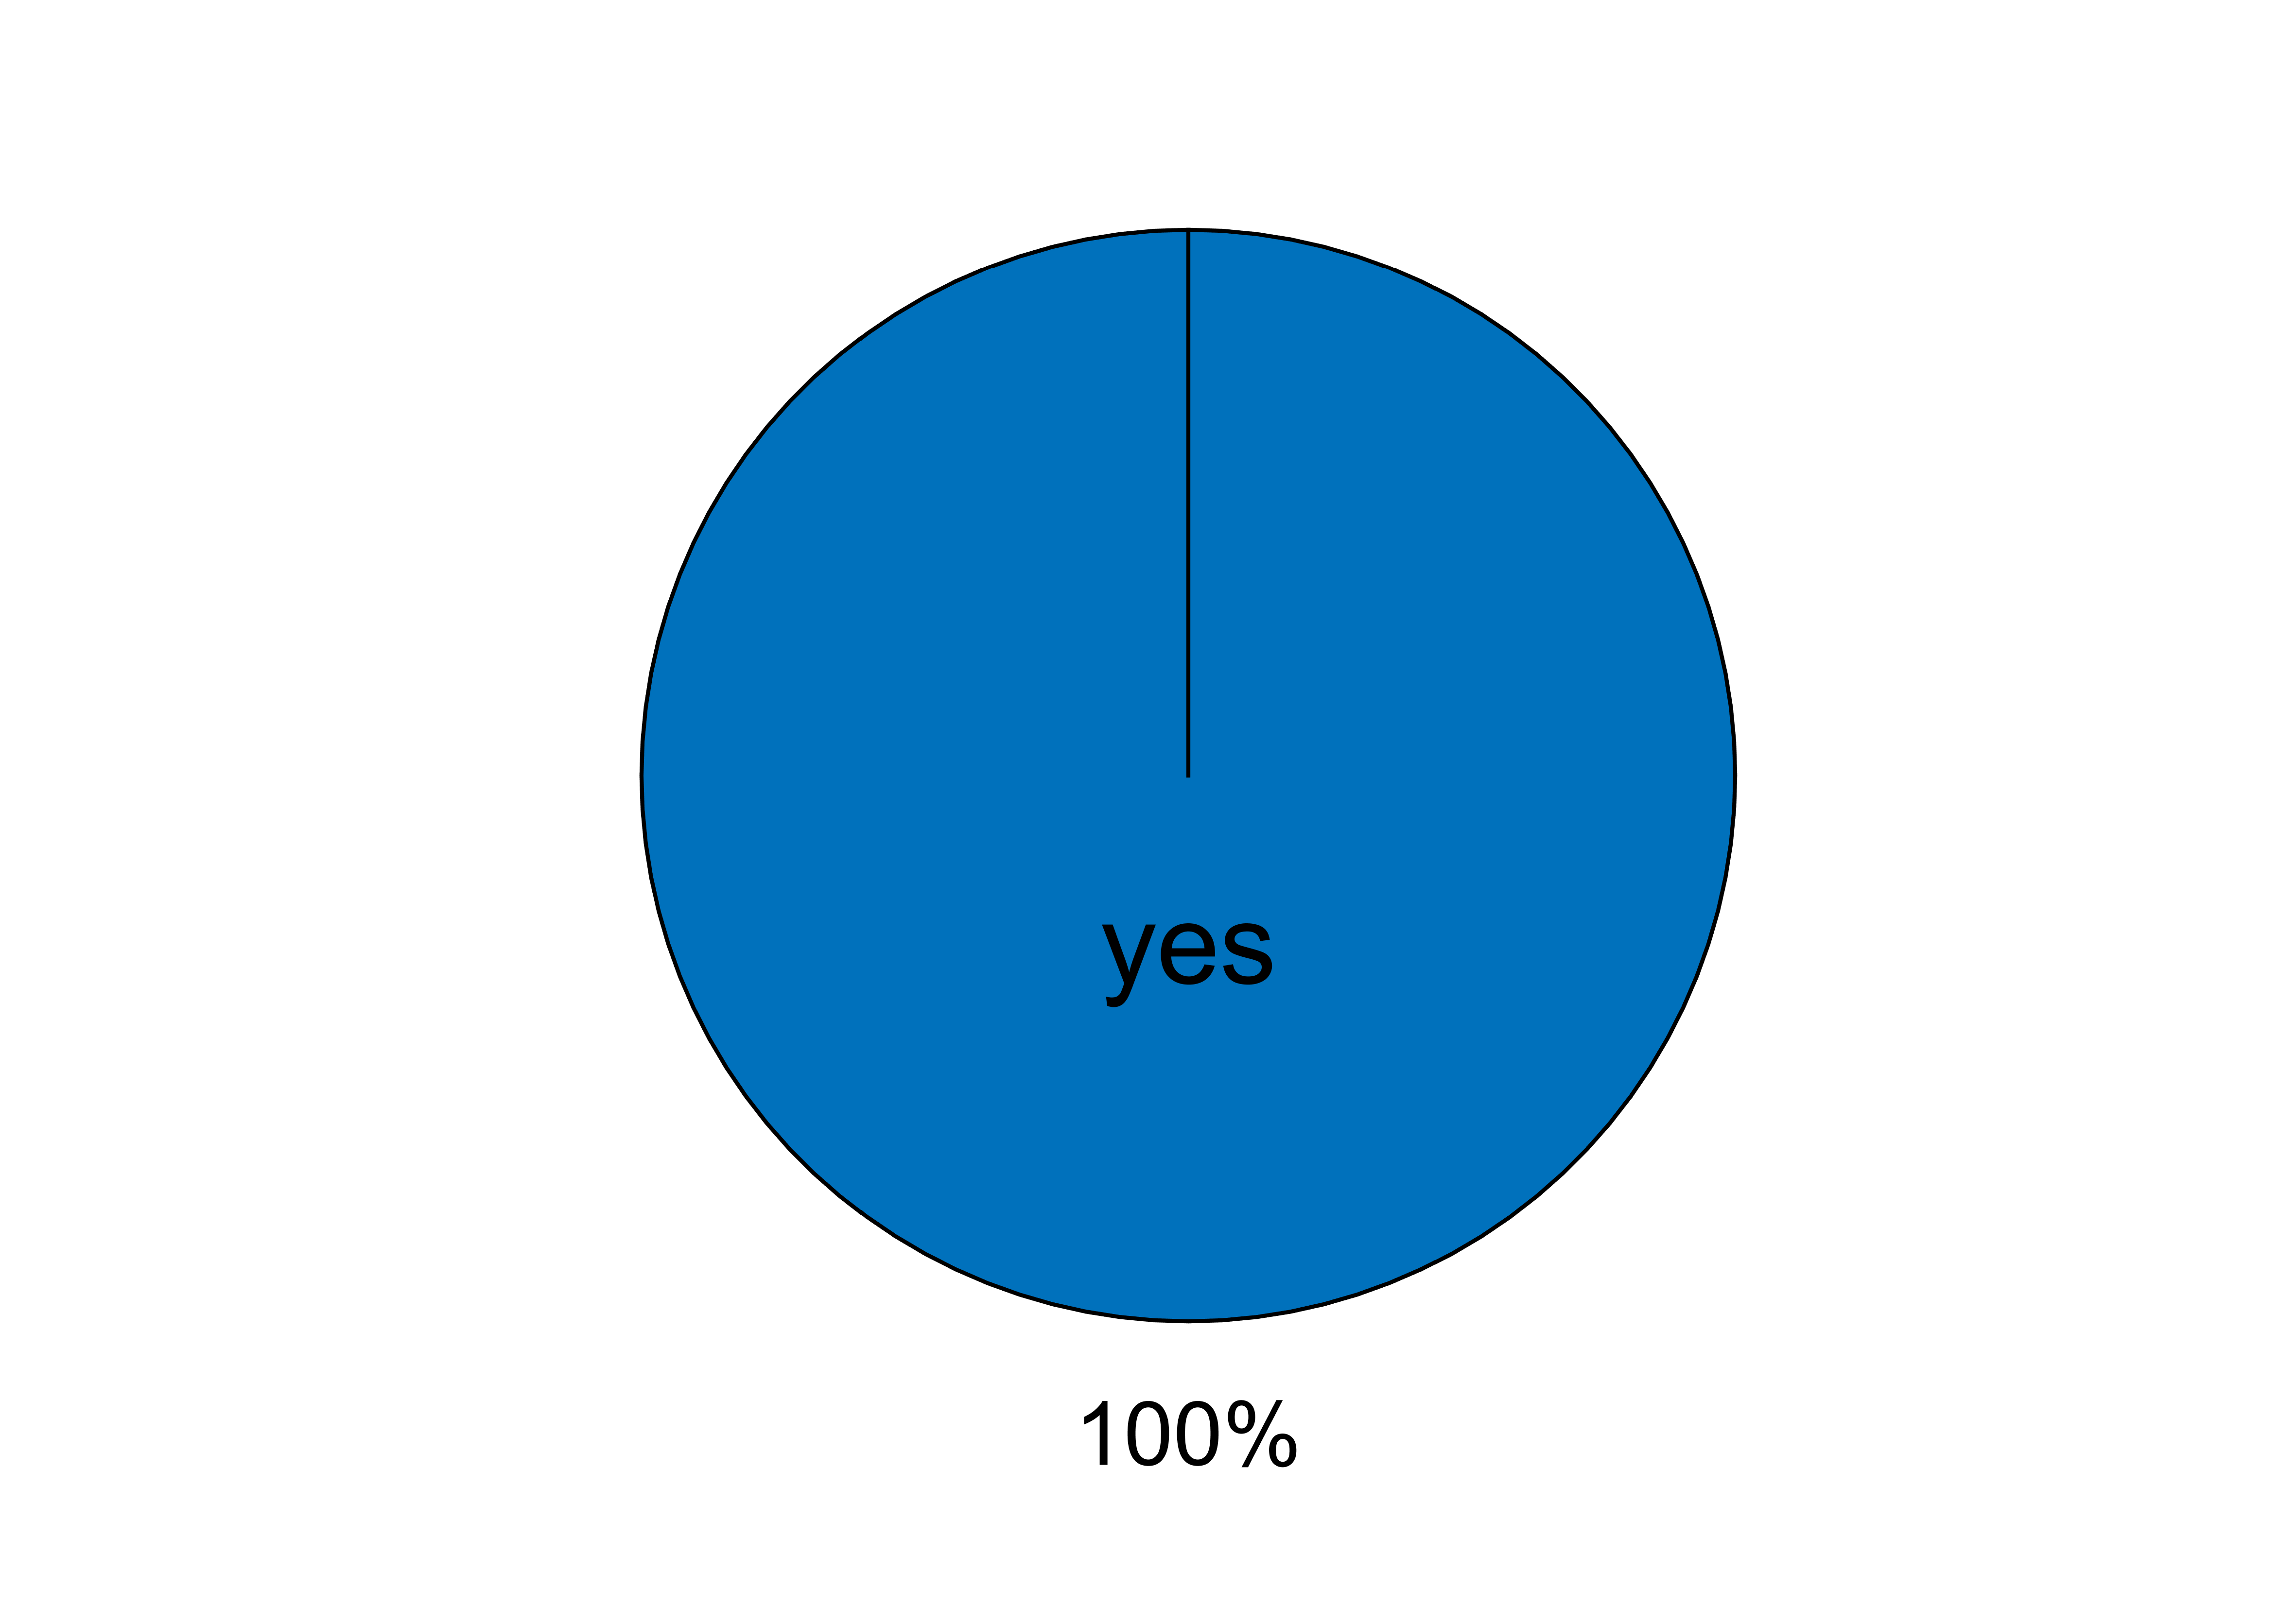
\includegraphics[width=\textwidth, trim={1.5cm 0.6cm 1.5cm 0.2cm}, clip]{T1_1.png}
		\caption*{\textbf{Q5:} "Do you own a smartphone?" \vspace{2mm}}
	\end{subfigure} \hspace{5mm}
	\begin{subfigure}[b]{0.45\textwidth}
		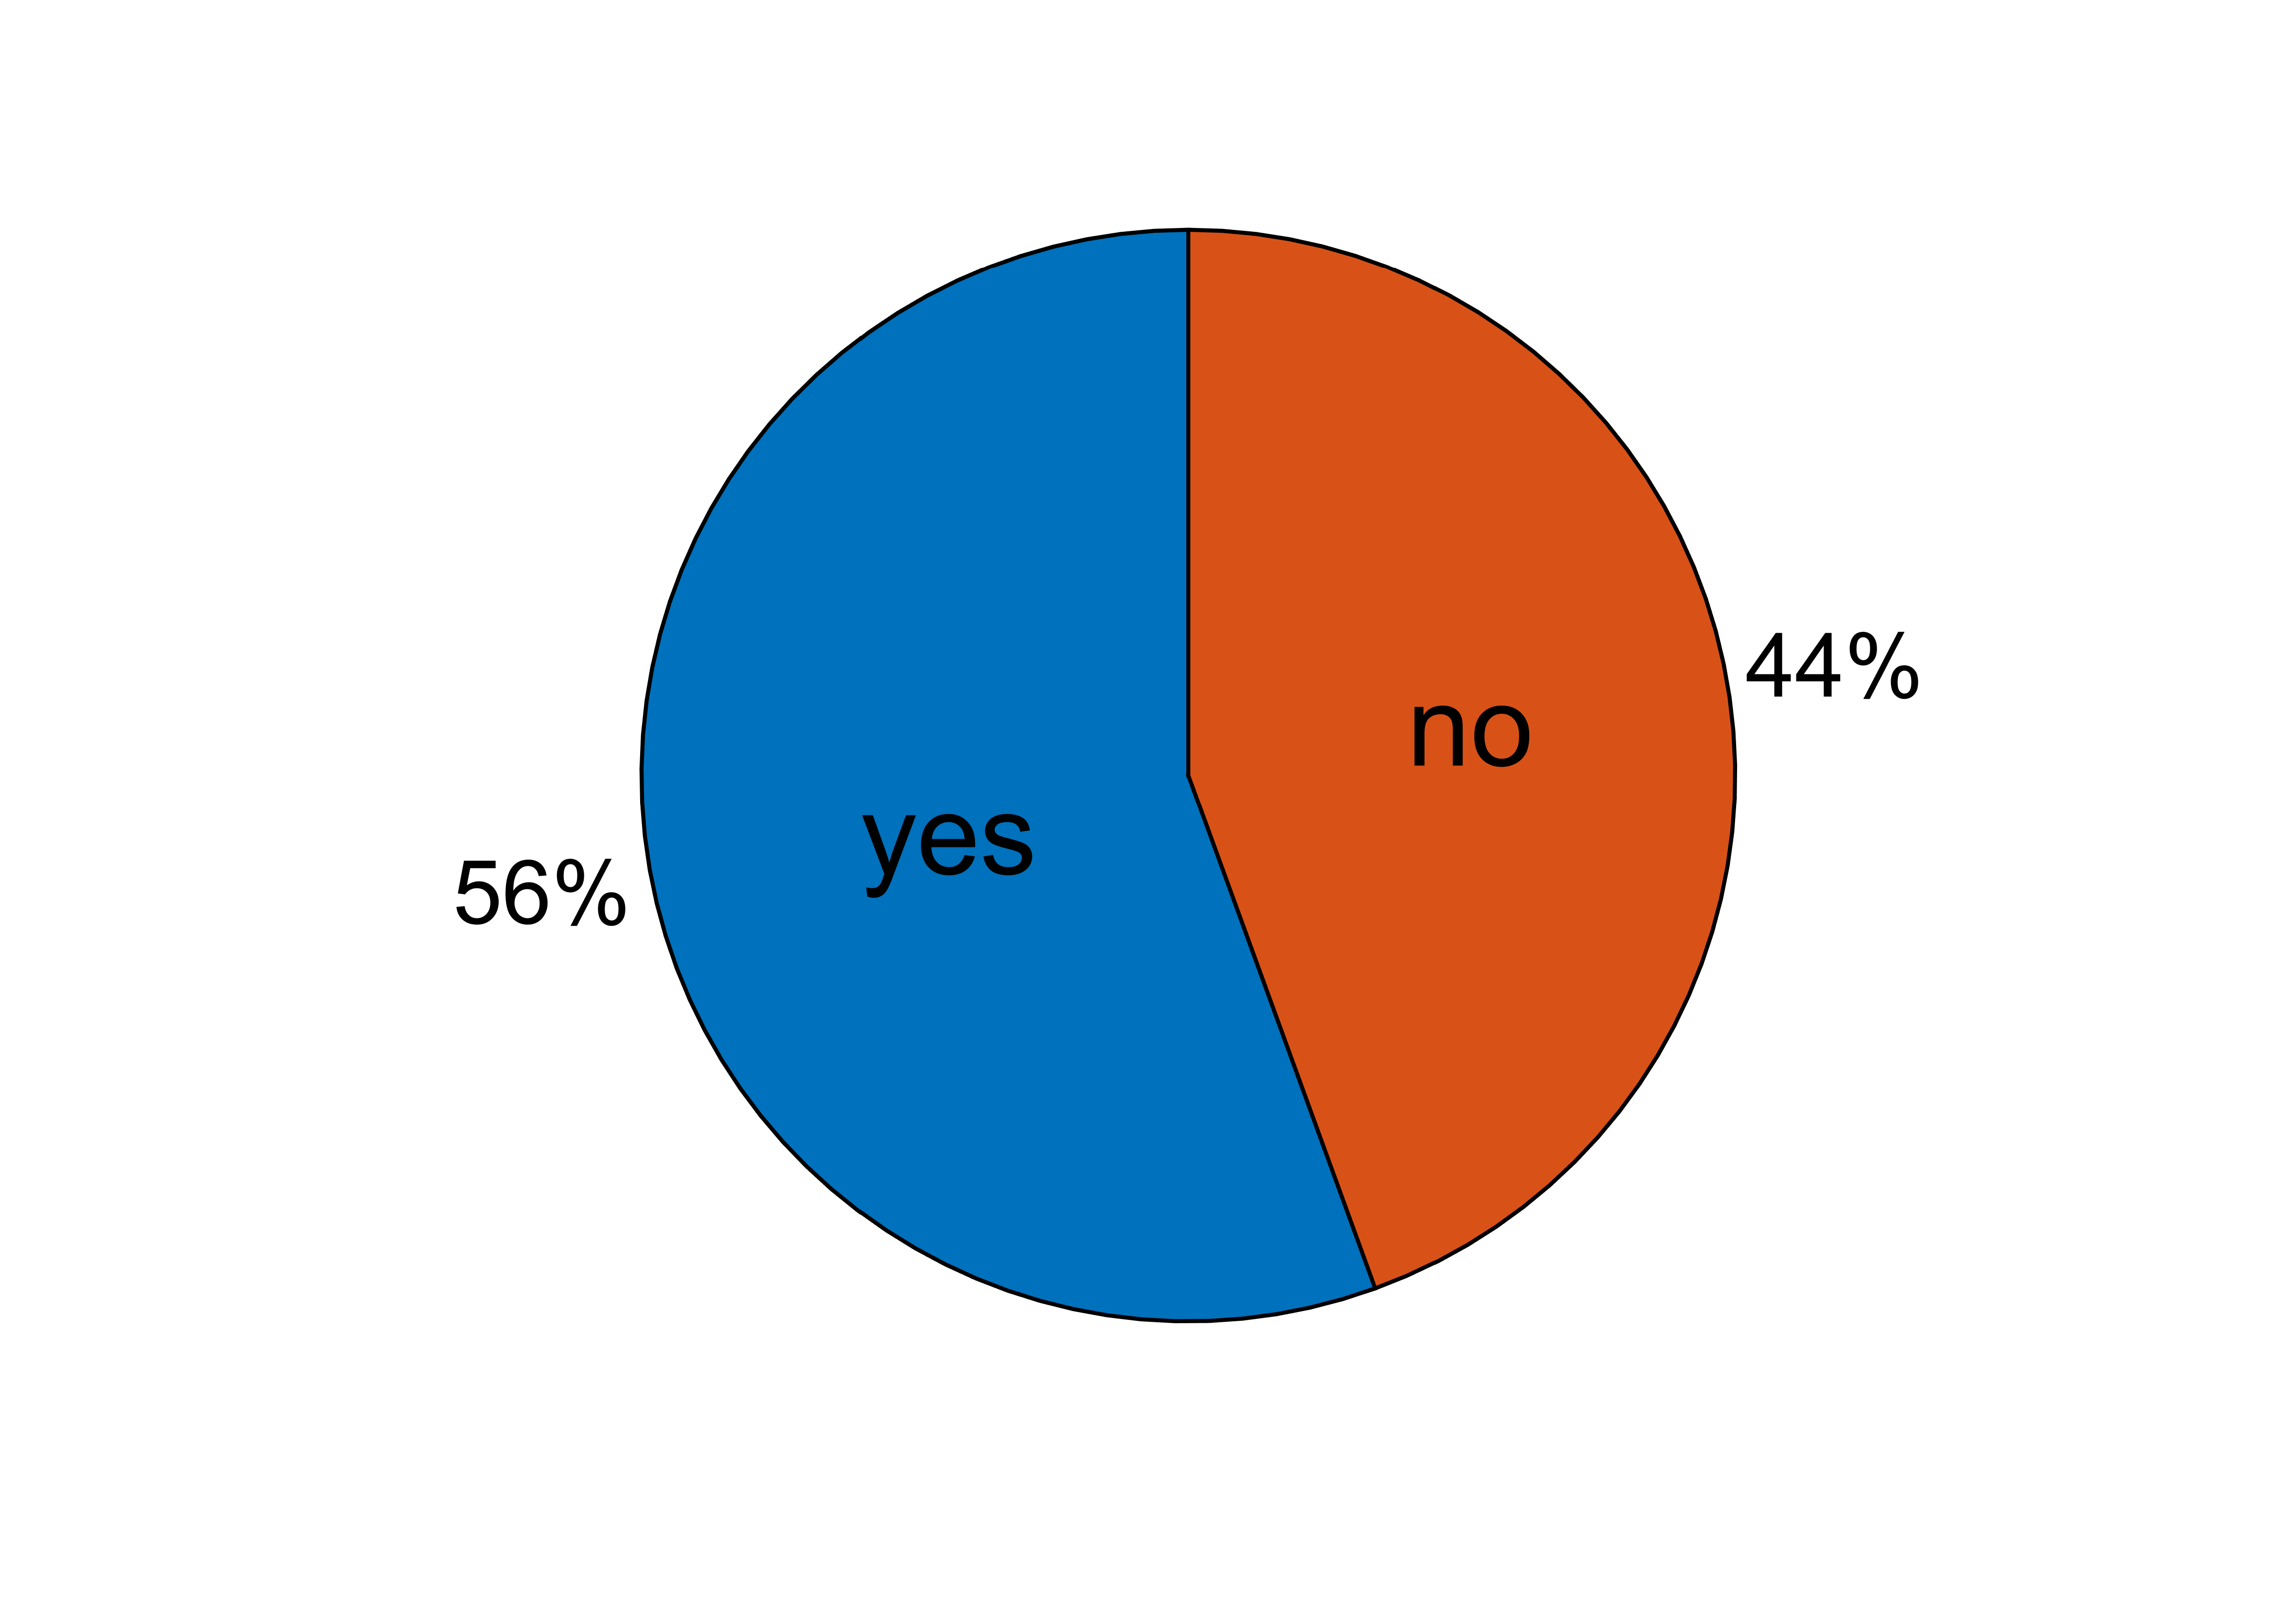
\includegraphics[width=\textwidth, trim={1.5cm 0.6cm 1.5cm 0.2cm}, clip]{T1_2.png}
		\caption*{\textbf{Q6:} "Do you own a tablet?" \vspace{2mm}}
	\end{subfigure}
	\begin{subfigure}[b]{0.45\textwidth}
		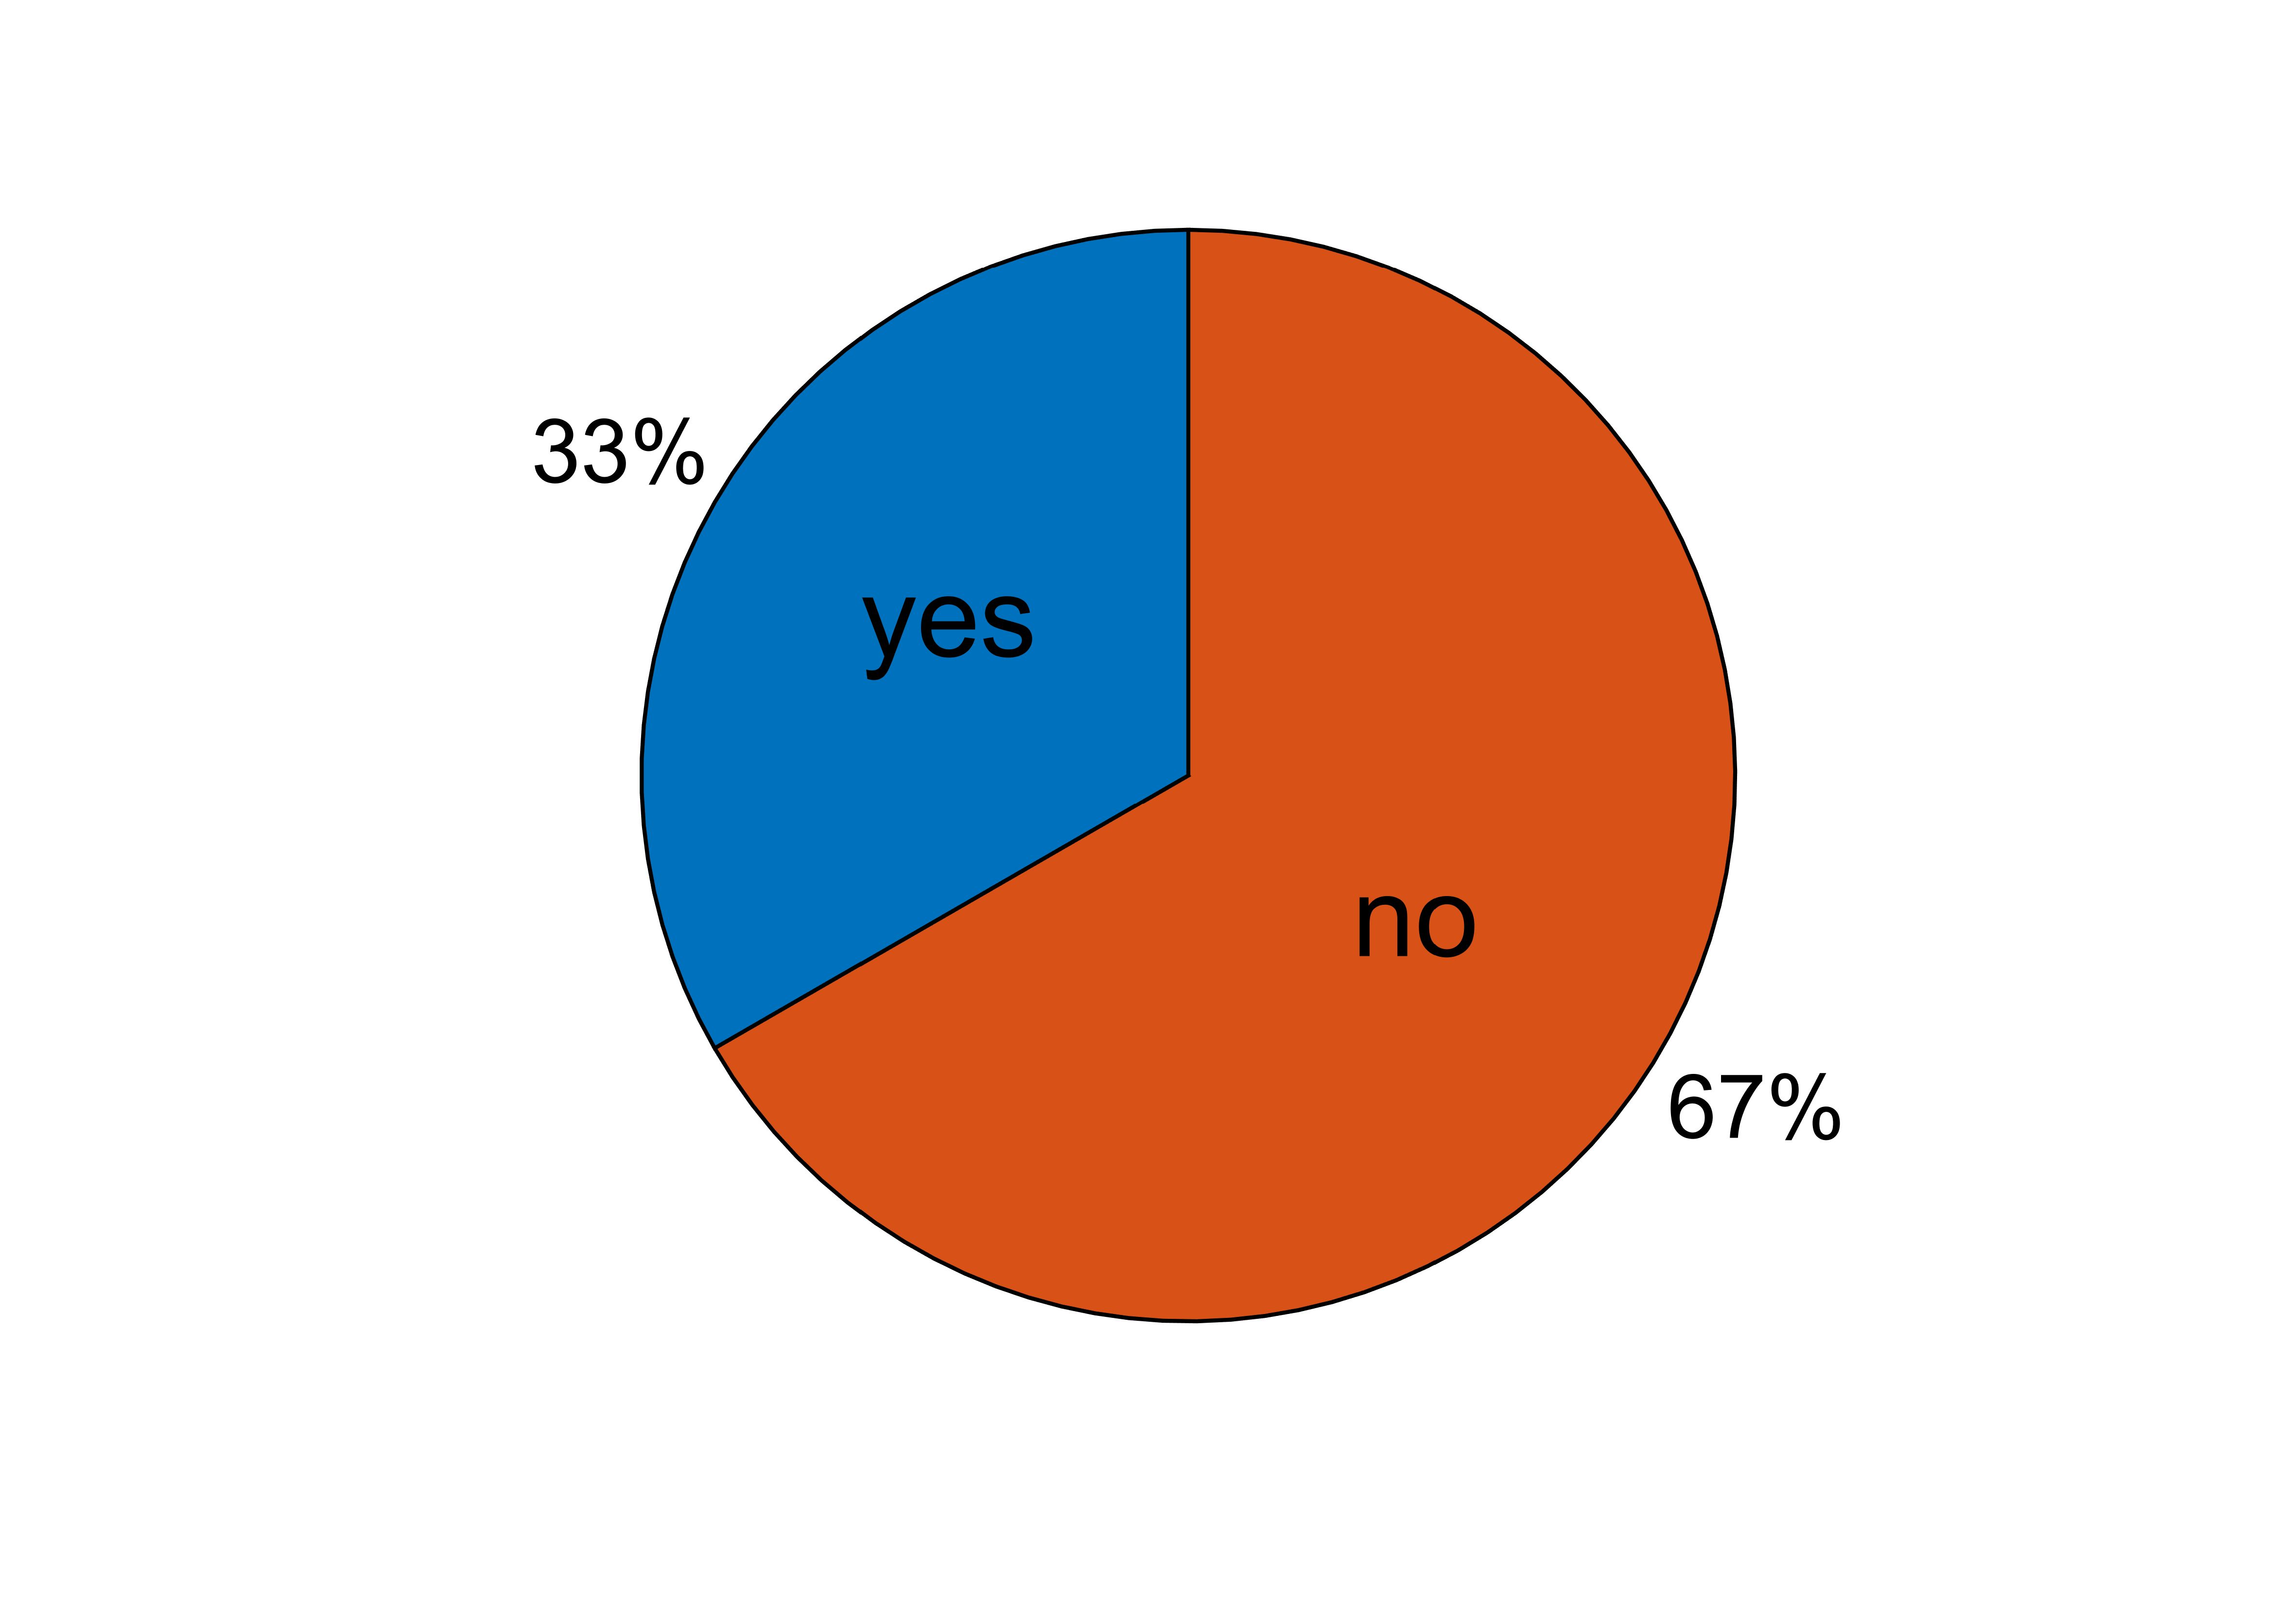
\includegraphics[width=\textwidth, trim={1.5cm 0.6cm 1.5cm 0.2cm}, clip]{T1_3.png}
		\caption*{\textbf{Q8:} "Have you previously used an application or service that uses automatic speech recognition?"} 
	\end{subfigure} \hspace{5mm}
	\begin{subfigure}[b]{0.45\textwidth}
		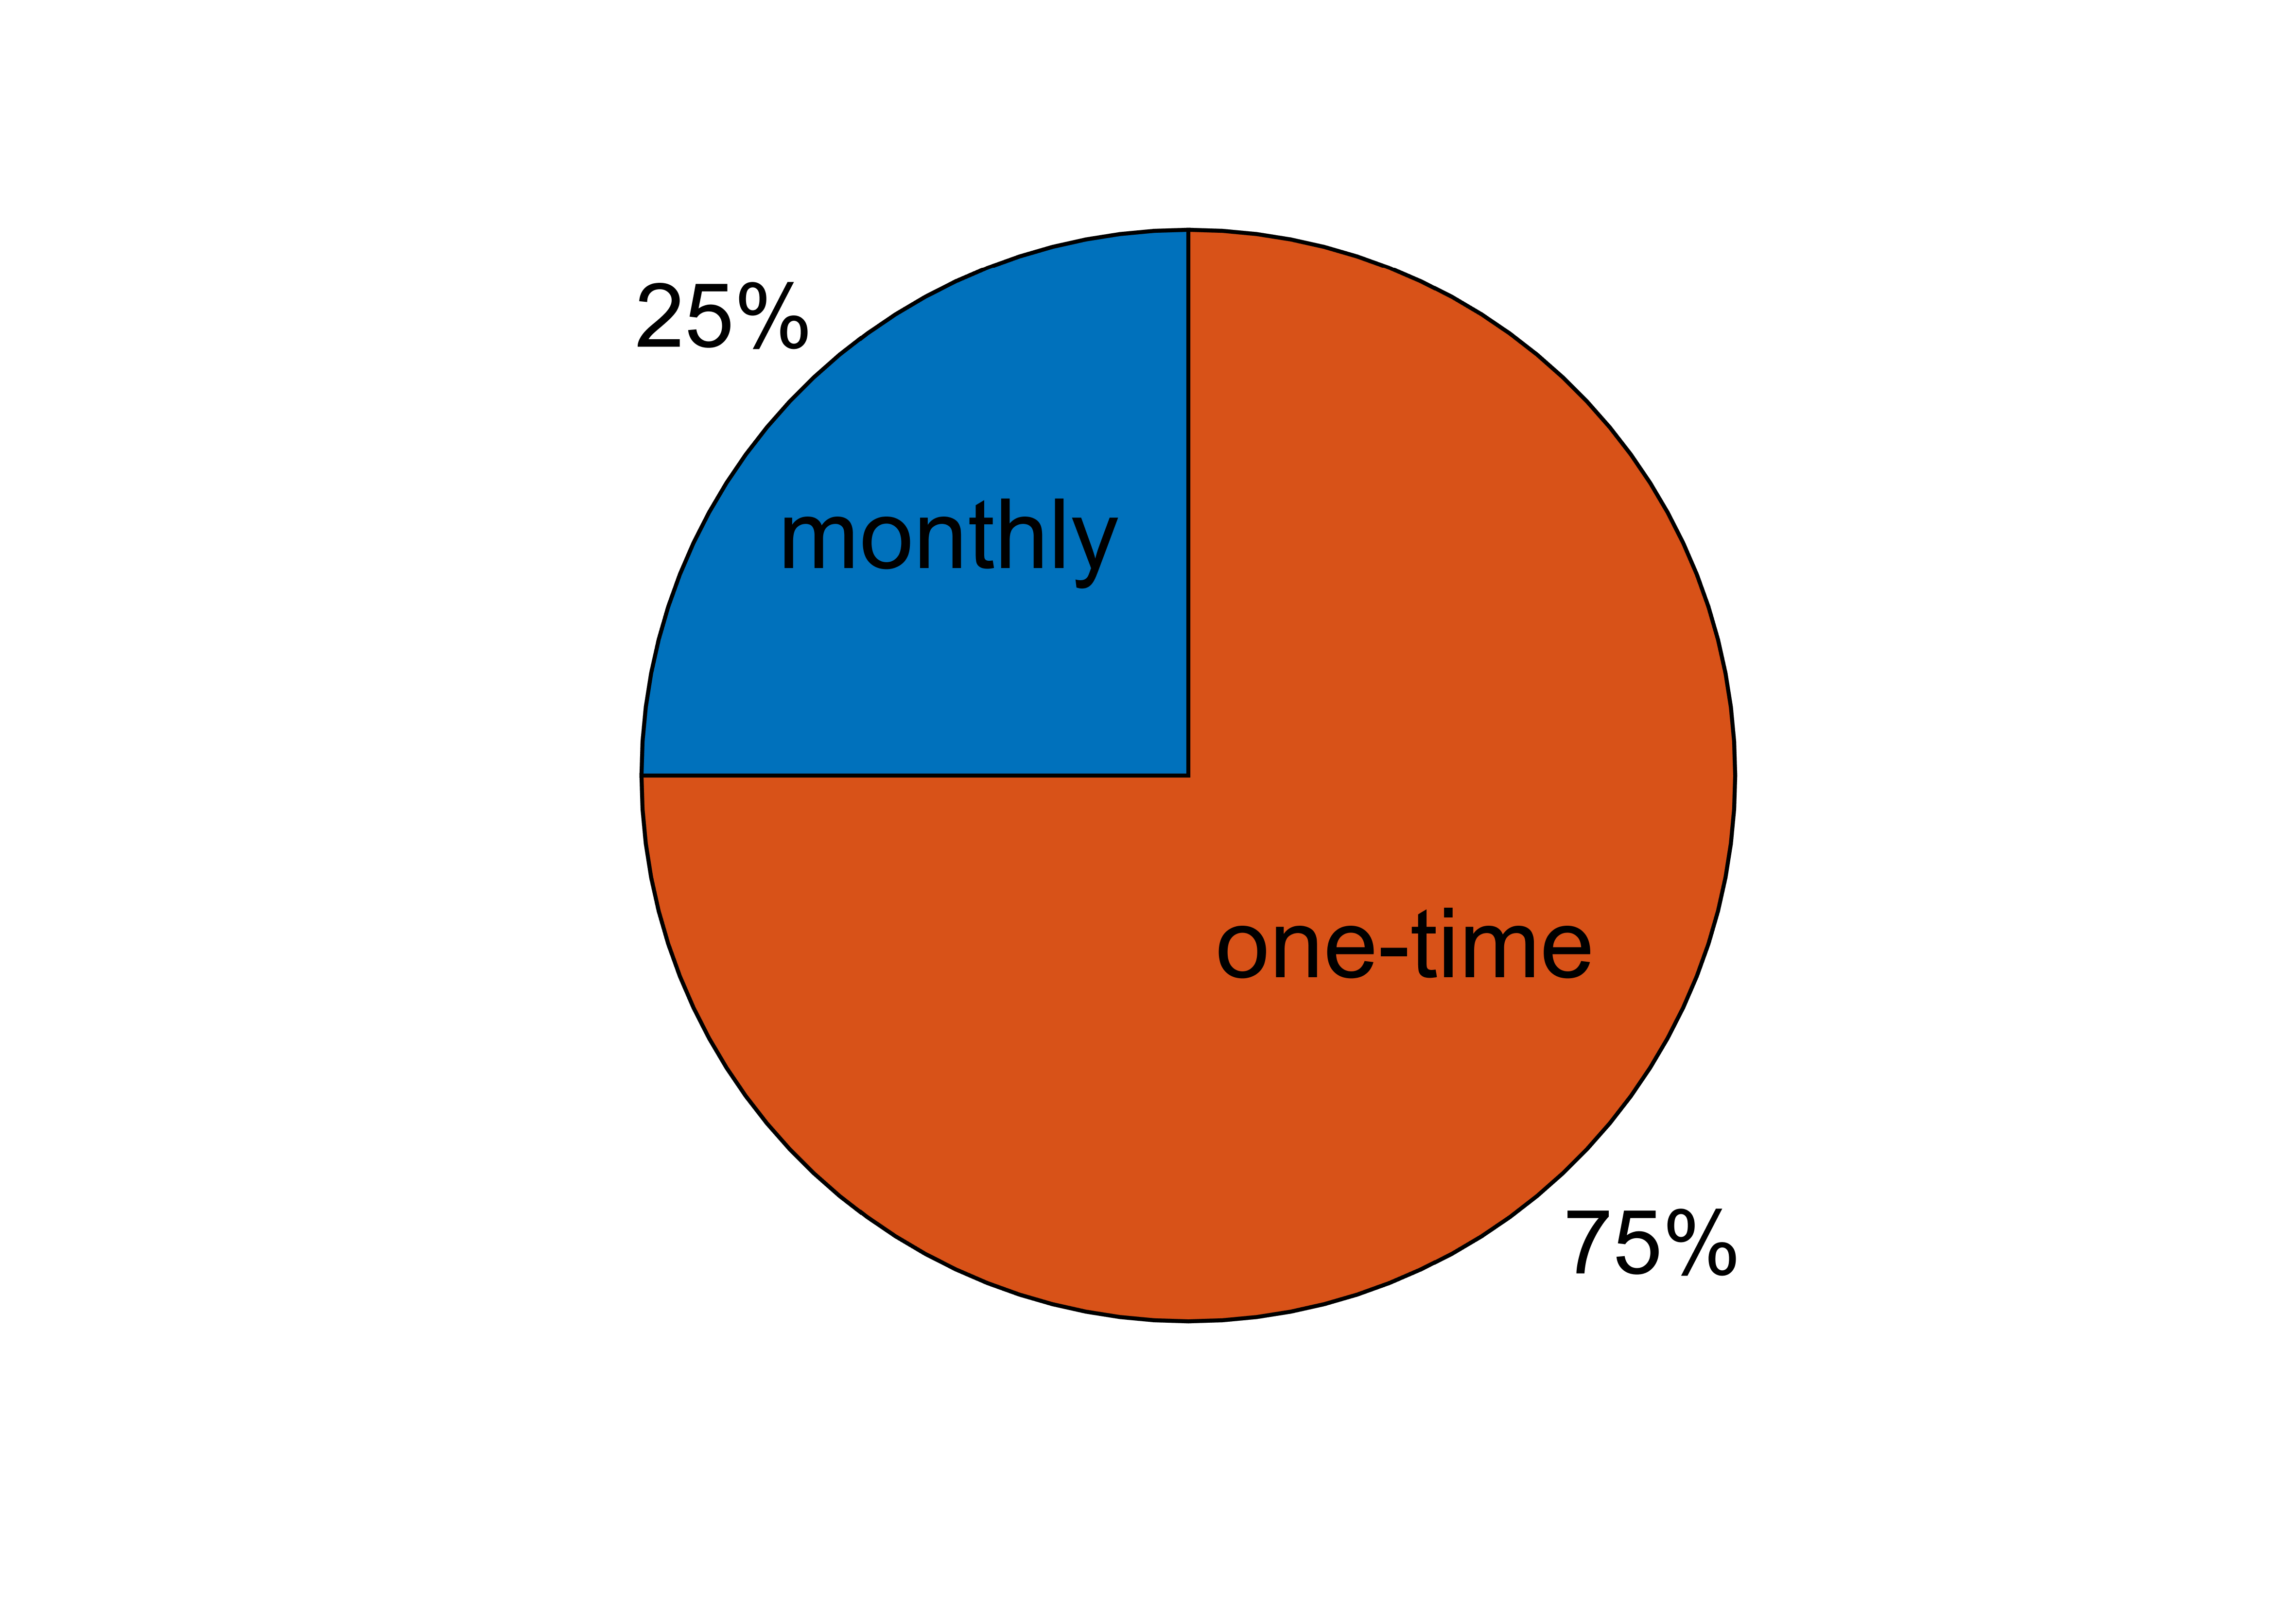
\includegraphics[width=\textwidth, trim={1.5cm 0.6cm 1.5cm 0.2cm}, clip]{T1_4.png}
		\caption*{\textbf{Q32:} "Would you rather pay a monthly fee or a one-time payment for an application like the Conversation Assistant?"} 
	\end{subfigure}
	\vspace{4mm}
	\caption{Binary questions from all sections.}
	\label{fig:results_pie} 
\end{figure}
The first three of these questions were from the introduction section's background questionnaire (Q5, Q6, Q8), and the fourth from the debriefing section (Q32). All test participants owned a smartphone, and a little over half owned a tablet (five out of nine).

\subsection{Numerical values}

The numerical data obtained, i.e., the numerical ratings given by the test participants, are presented with a box plot for each question, divided by the section. The actual numbers given by the test participants for each question are included in appendix \ref{sec:answers}, and the MATLAB code in appendix \ref{sec:matlab}. In the box plots, the (red) central mark represents the median value. The bottom of the box (in blue) corresponds to the 25th percentile, and the top of the box to the 75th percentile. It should be noted that when the median is not centered in the box, it shows sample skewness, meaning the values are distributed asymmetrically. The lines (in black) extending from the box display the range of all values that are not considered outliers. A value is judged to be an outlier and marked with a red cross if it is more than 1,5 times the interquartile range (i.e., the size of the box) away from the top or bottom of the box. \cite{boxplot} \\\\
Figure \ref{fig:results1} presents the data from the background questionnaire, which consists only of one question measuring the self-perceived proficiency with computers and mobile devices. 
\begin{figure}[b!]
	\centering
	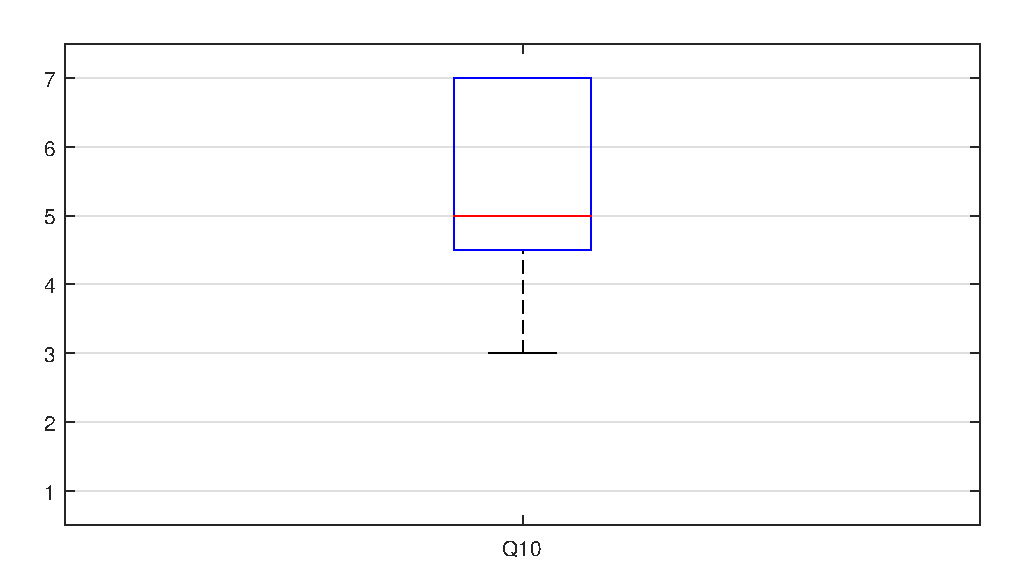
\includegraphics[width=\textwidth]{T2_box1.pdf}
	\caption{Question 10: "In your own opinion, how proficient are you at using computers and mobile devices in everyday life?"}
	\label{fig:results1} 
\end{figure}
The question was included in order to get a rough estimate for how much experience the participant has with these devices and how comfortable they are with technology in general. The subjective wording in the assessment served a purpose as well: Someone who feels that they are good with smart devices likely has a very positive attitude towards technology, regardless of how much knowledge and skill they might actually possess.  Conversely, someone who rates their skills very low likely has some aversion and negative expectations towards technology, even if their skills might actually be relatively comparable to someone with a higher rating. Therefore, the answers to this question, together with the other background questions, can be quite useful for better understanding the answers to other questions. For example, if an experienced user thinks the application is easy to use, it might not tell that much about its actual ease-of-use, especially for novices. Whereas, if someone who feels they are very bad at using computers thinks the application is very easy to use, the opinion has much more weight to it. In the same way, if a skilled participant, who owns both a smartphone and a tablet thinks the application is really hard to use, then it most probably is. If a person with a low reported proficiency thinks it's hard to use, it can be more due to their lack of experience with these devices and negative attitude, instead of any design flaws in the application itself. The question also served as a gentle introduction to the questionnaire's format and functioning, preparing and giving the participants some practice with it before moving on to the main questions. \\\\
Figure \ref{fig:results2} presents the data from section one of the user test. The questions were the following:
\begin{description}
	\item[Q11] Did the Conversation Assistant help you to understand speech? \\ \textit{(not at all -- very much)}
	\item[Q12] Was using the Conversation Assistant easy? \\ \textit{(not at all -- very easy)}
	\item[Q13] Did using the Conversation Assistant make it harder to follow speech? \\ \textit{(not at all -- very much)}
	\item[Q14] Was the speech recognition fast enough? \\ \textit{(too slow -- fast enough)}
	\item[Q15] Were the speech recognition results accurate enough (speech was recognized correctly)? \\ \textit{(unusable -- good enough)}
\end{description}
\begin{figure}[h!]
	\centering
	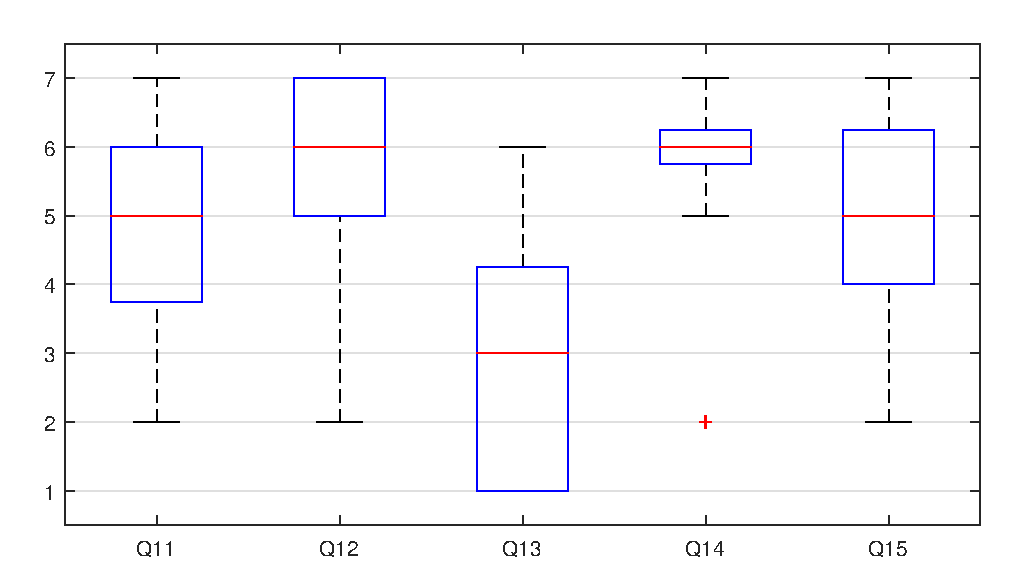
\includegraphics[width=\textwidth]{T2_box2.pdf}
	\caption{Section 1 results.}
	\label{fig:results2} 
\end{figure}
Figure \ref{fig:results3} presents the data from section two of the user test. The questions were the following:
\begin{description}
	\item[Q16] Did the Conversation Assistant help you to understand speech? \\ \textit{(not at all -- very much)}
	\item[Q17] Was using the Conversation Assistant easy? \\ \textit{(not at all -- very easy)}
	\item[Q18] Did using the Conversation Assistant make it harder to follow speech? \\ \textit{(not at all -- very much)}
	\item[Q19] Did using the Conversation Assistant slow down the conversation? \\ \textit{(not at all  -- very much)}
	\item[Q20] Was the speech recognition fast enough? \\ \textit{(too slow -- fast enough)}
	\item[Q21] Were the speech recognition results accurate enough (speech was recognized correctly)? \\ \textit{(unusable -- good enough)}
\end{description}
\begin{figure}[h!]
	\centering
	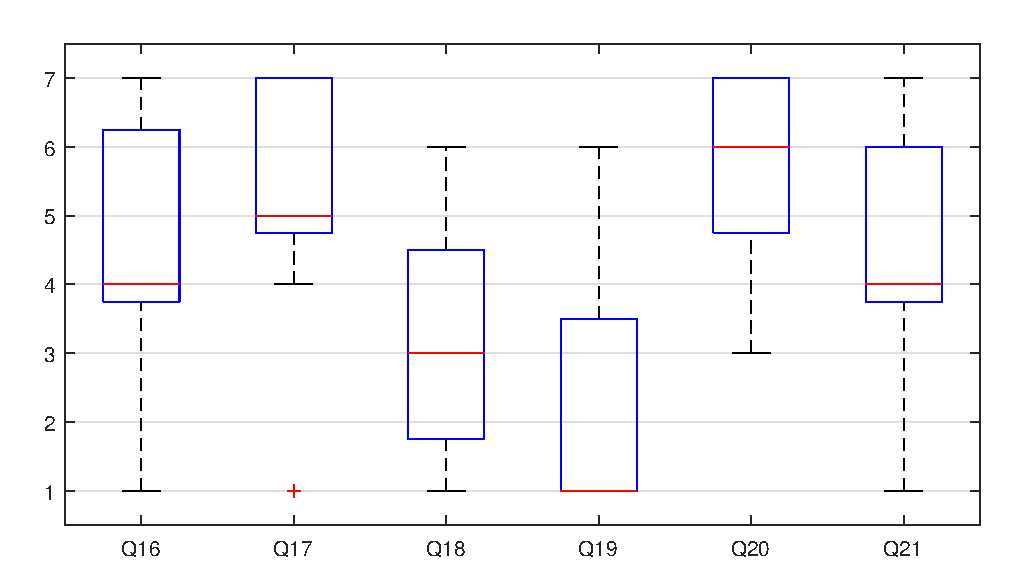
\includegraphics[width=\textwidth]{T2_box3.pdf}
	\caption{Section 2 results.}
	\label{fig:results3} 
\end{figure}
Figure \ref{fig:results4} presents the data from the debriefing. The questions were the following:
\begin{description}
	\item[Q22] Was the Conversation Assistant useful in test situations? \\ \textit{(not at all -- very much)}
	\item[Q23] Do you consider it to be important that the size and color of the font can be freely adjusted? \\ \textit{(not at all -- very important)}
\end{description}
\begin{figure}[h!]
	\centering
	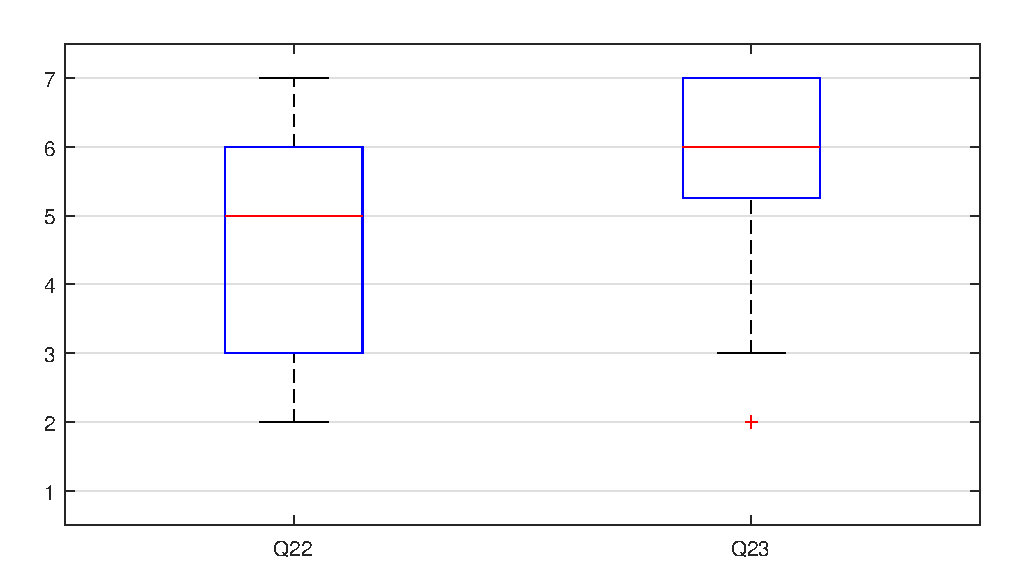
\includegraphics[width=\textwidth]{T2_box4.pdf}
	\caption{Debriefing results.}
	\label{fig:results4} 
\end{figure}
Figure \ref{fig:results4} presents the results for how much the participants would be ready to pay monthly or as an one-time purchase for an application like the Conversation Assistant?
\begin{figure}[h!]
	\centering
	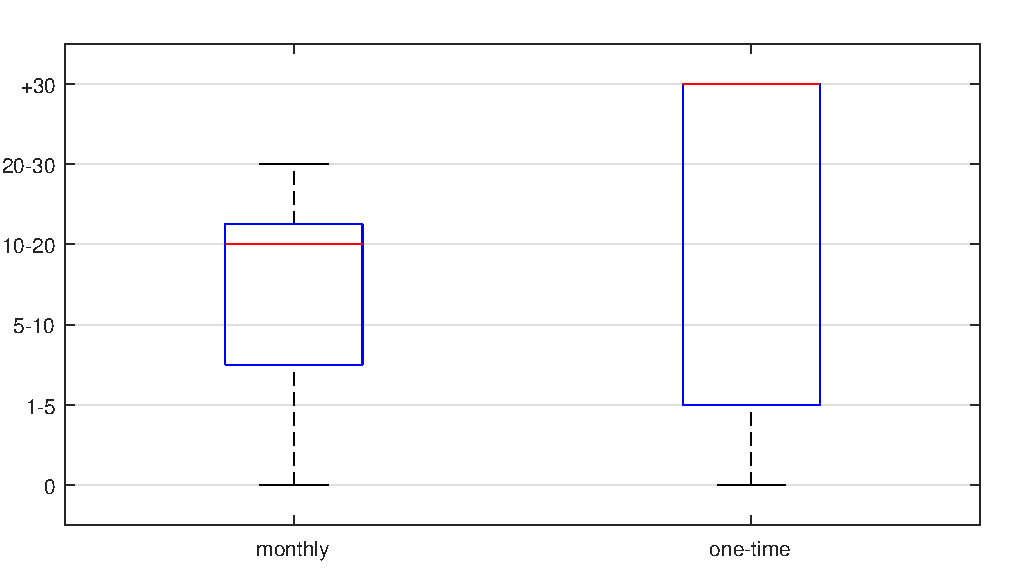
\includegraphics[width=\textwidth]{T2_box5.pdf}
	\caption{"How much would you be ready to pay for an application like the Conversation Assistant?". Price in euros.}
	\label{fig:results5} 
\end{figure}

\subsection{Verbal feedback}

\subsection{Analysis}  

One factor to keep in mind when analyzing the results is that the people who participated in the testing showed enough interest towards the Conversation Assistant to take part in the testing, meaning the test participants have to be viewed as inherently biased in some small degree towards the application. It seems probable that someone with no interest towards this type of assistive application would most probably not participate in testing it either.

\clearpage

\section{Conclusions} \label{sec:loppu}

Based on the reported substantial, and increasingly growing prevalence of hearing loss, new and affordable solutions for lessening the negative effects hearing impairment are urgently needed. \\\\
During the user testing, one of the test participants had a written language interpreter with her, as she was complete deaf and didn't use any hearing devices. This offered a good opportunity to informally compare the Conversation Assistant with a human, professional speech to text translator. The translator had a laptop computer that was placed next to the Conversation Assistant laptop on the table in front of the test user. The translator had a wireless keyboard that she used to write text to the screen, and the end result was effectively and visually pretty similar to the Conversation Assistant. During the introduction phase and between the test sections, both laptops were simultaneously displaying the translations, the other produced by our ASR system, and the other by the human translator. The human translator paused during the actual testing of course. Based on this brief empirical observation, the Conversation Assistant seemed to be already noticeable faster than a human translator, but accuracy was still relatively far off from a human for conversational speech. However, it was interesting to note that the human translation results were far from perfect as well, also containing surprisingly many errors especially in the spelling. The most probable explanation seems that accurate translation has to be sacrificed for speed. All things considered, the Conversation Assistant didn't seem to be too far off from the performance level of a professional human translator. One area, where human translators are by far superior is that they can easily add relevant information to the translation, such as who is speaking (to whom), describing the mood or tone of voice, and also translate other sounds in addition to speech. While arguably a human translator is still better overall in speech to text translation for the hearing impaired, it takes many years of training and practice for a human translator to achieve these results. Also, one person cannot be in many places at the same time and requires monetary compensation for ones time and skills, meaning very few individuals can actually benefit from those translation services in the grand scheme of things. On the contrary, once an excellent ASR model is trained, it can be copied infinitely and used all the time in every place with practically no additional costs, enabling the best achieved level of automatic speech recognition for all very cheaply. \\\\
This first round of user testing also ended up being the only one. At the beginning of the project, two or more rounds of testing were envisioned originally. However, after the first round of testing, more iterations of the same test setup were deemed redundant without significant changes to the Conversation Assistant, which in turn was not possible within the scope of this thesis. Expanding the test setting from a one-on-one conversation to a group conversation would have been the ideal next step, but unfortunately there wasn't enough time for it at this stage. Many test subjects reported that in one-on-one conversations were they can see the other person well can be quite easy to follow, even if they don't hear other person very well, by using traditional methods like lip-reading. This in turn led many of the test subjects to speculate that the Conversation Assistant would be much more useful in group conversations and in situations where the speaker is farther away or lip-reading is otherwise not possible. Examples given of the latter situations included lectures and video-conferencing meetings. \\\\
Staging a group conversation session would bring along many new complications and practical challenges compared to the relatively simple case of having just one test subject and one person running the test. There are also some unresolved technical challenges, like ensuring good quality audio input from all speakers without complicated microphone setups involving multiple microphones. \\\\
Technology is there but no wide-spread applications yet? \\\\
Better than old solutions and human interpreters? Speech recognition very fast \cite{mcgraw2016personalized}. \\\\
Even if not completely solving it. \\\\
Machine learning enabling progress in all devices. \\\\
An assistive application like the presented Conversation Assistant prototype could not only improve the quality of life for hearing impaired persons and the people close to them, but also contribute towards a more inclusive society and even bring about wider socio-economic benefits to all as a consequence.

\subsection{Future work}

More testing. Better models for conversation speech. As they say: "There's no data like more data." \\\\
Group testing. \\\\
How useful depending on level of hearing impairment! \\\\
Web and mobile application, server-based recognizer. \\\\
Microphone methods: access other peoples mobile devices in meetings. Beamforming and directional long range mics. \\\\
Speaker diarization. \\\\
Augmented reality.

\clearpage

% References
\addcontentsline{toc}{section}{References}
\bibliographystyle{ieeetr}
\bibliography{references}

%% Appendices
\clearpage

\appendix

\section{Prototype Source Code} \label{sec:proto}

The source code of the Conversation Assistant prototype implemented with the Python programming language (version 3).

\inputminted[fontsize=\scriptsize]{python}{keskusteluavustin.py} % \tiny \scriptsize

\clearpage

\section{Questionnaire} \label{sec:kysely}

Printed pages of the questionnaire from the Google Forms web application used in the user testing.

\begin{figure}[H]
	\centering
	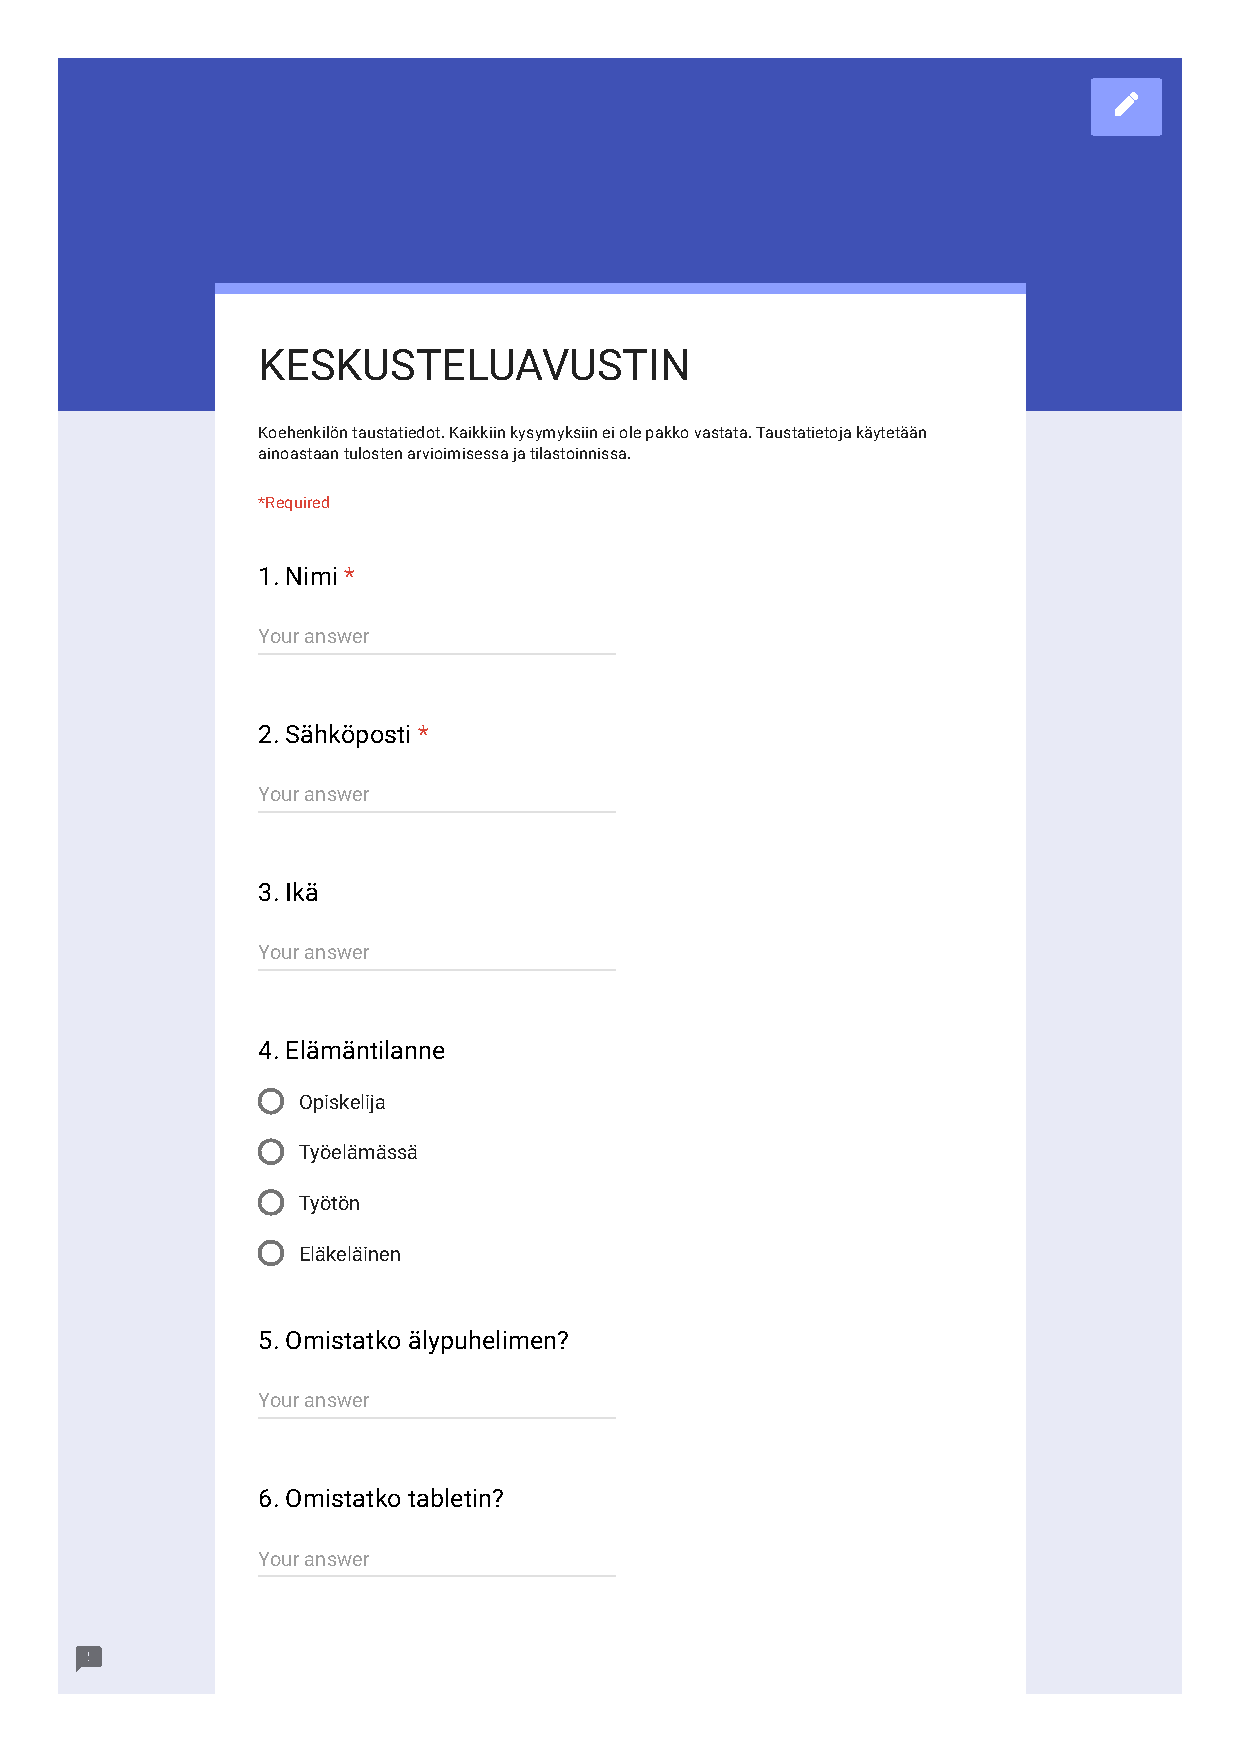
\includegraphics[page=1,trim={1cm 2cm 1cm 2.5cm}, clip, width=\textwidth]{q1.pdf}
\end{figure}
\begin{figure}
	\centering
	\includegraphics[page=2,trim={1cm 0cm 1cm 0cm}, clip, width=\textwidth]{q1.pdf}
\end{figure}

\begin{figure}
	\centering
	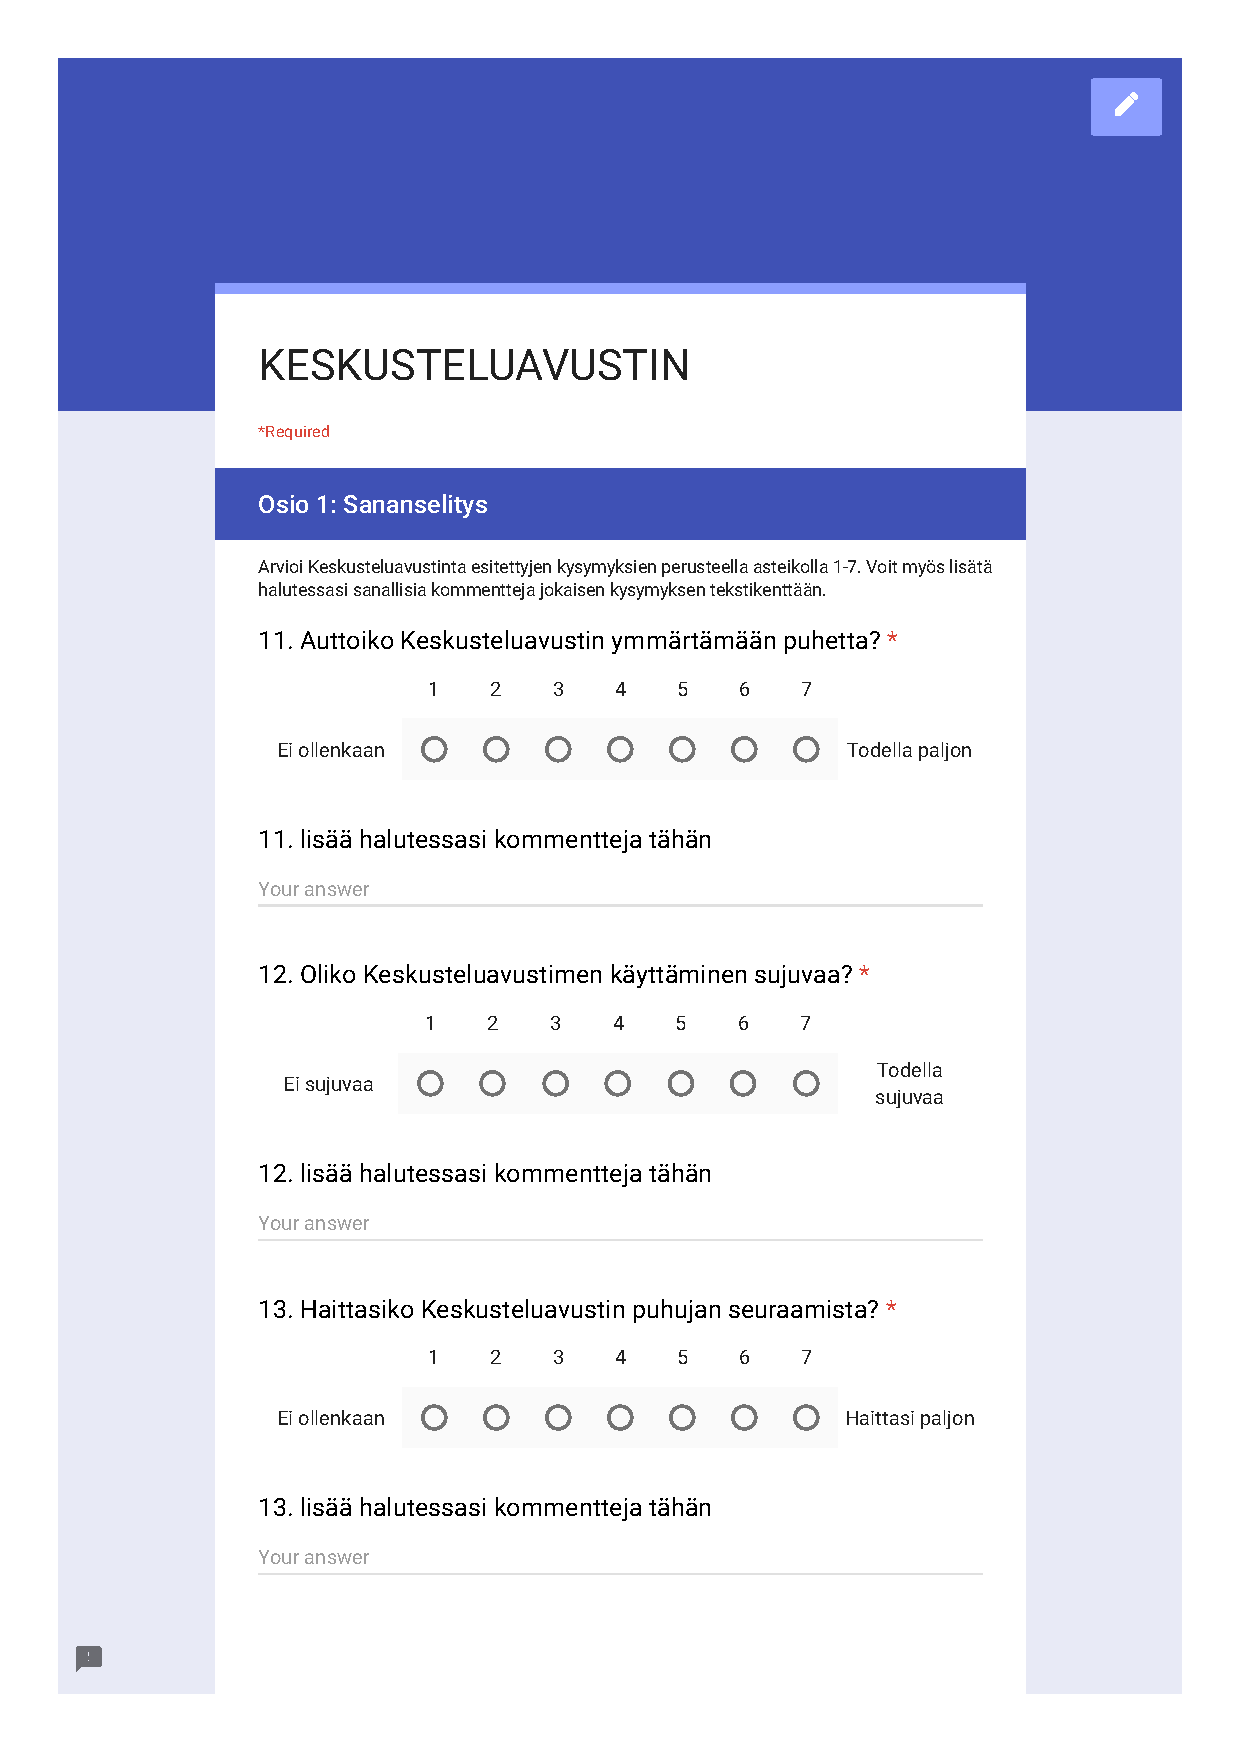
\includegraphics[page=1,trim={1cm 1cm 1cm 2.5cm}, clip, width=\textwidth]{q2.pdf}
\end{figure}
\begin{figure}
	\centering
	\includegraphics[page=2,trim={1cm 0cm 1cm 0cm}, clip, width=\textwidth]{q2.pdf}
\end{figure}

\begin{figure}
	\centering
	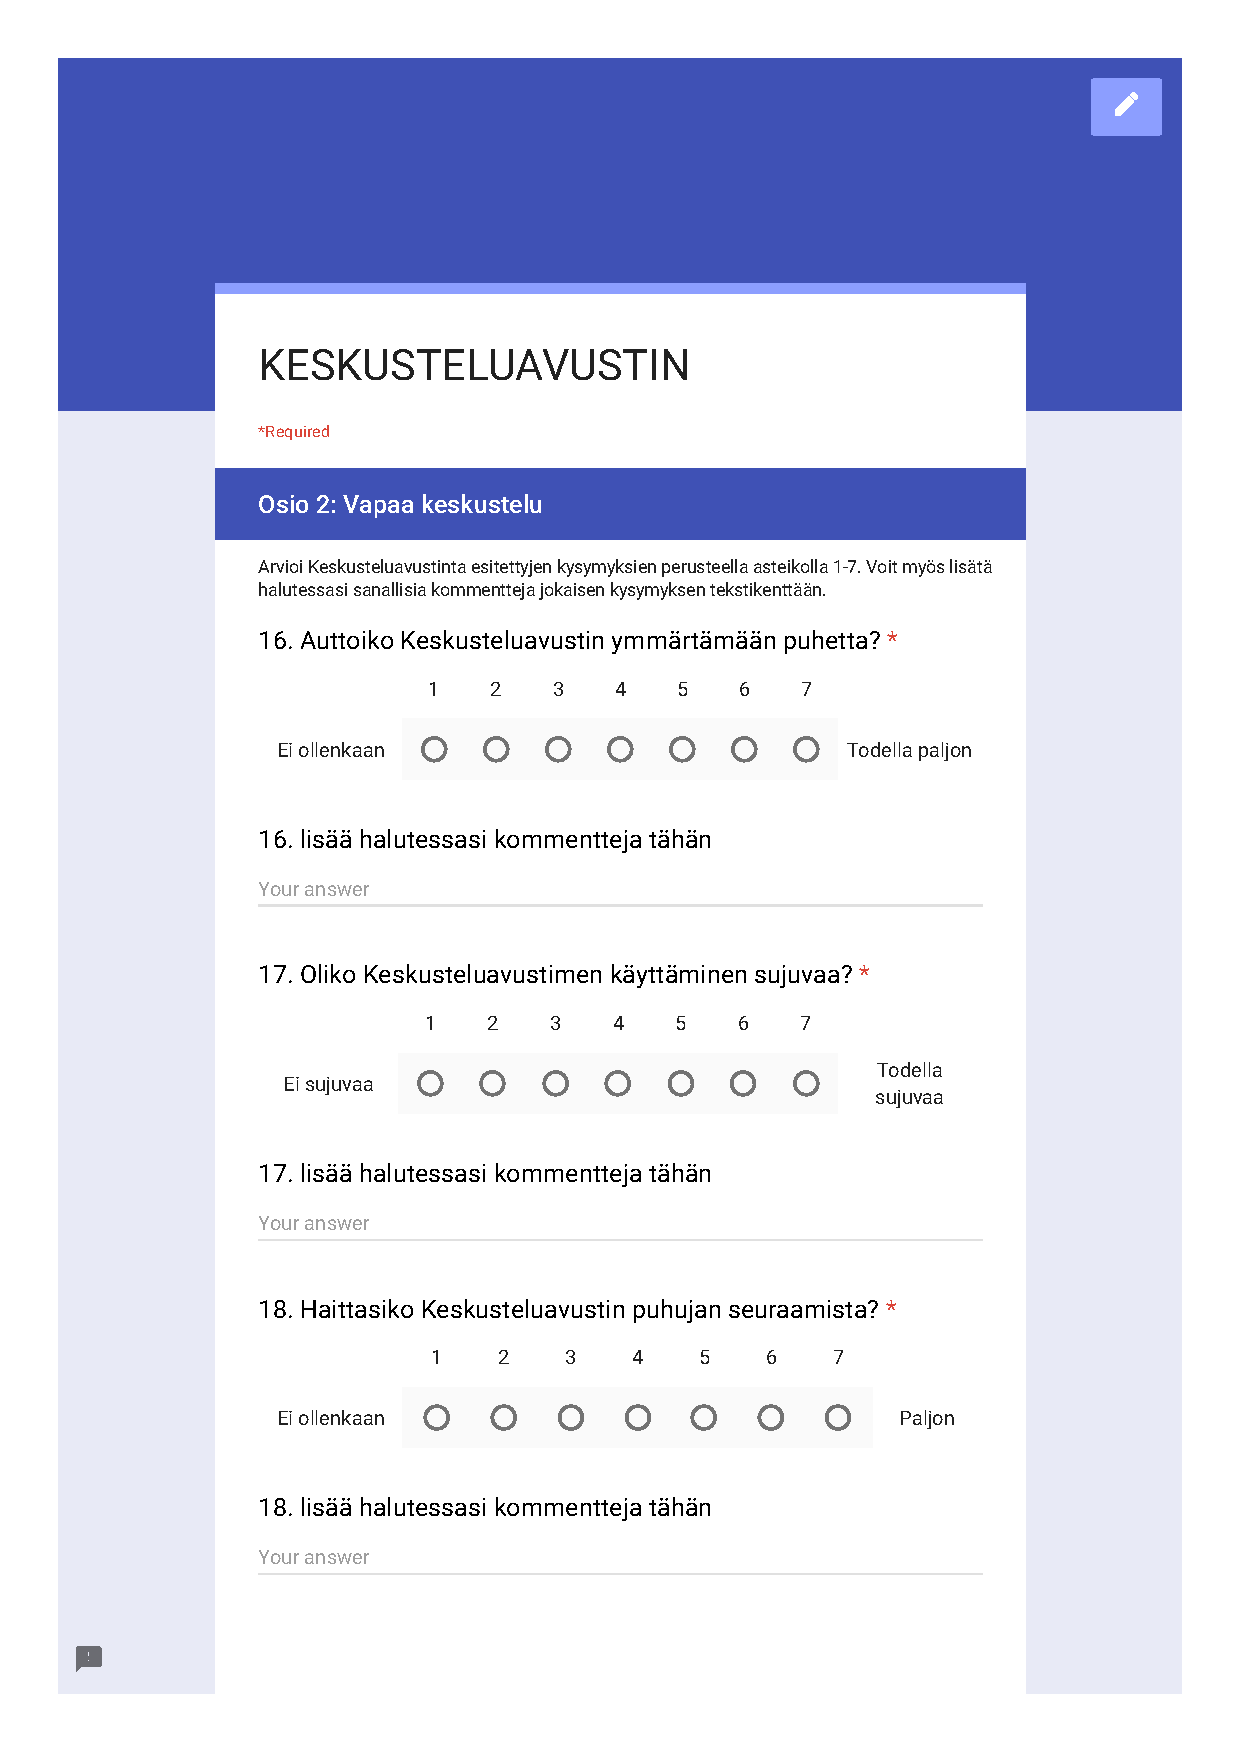
\includegraphics[page=1,trim={1cm 1cm 1cm 2.5cm}, clip, width=\textwidth]{q3.pdf}
\end{figure}
\begin{figure}
	\centering
	\includegraphics[page=2,trim={1cm 0cm 1cm 0cm}, clip, width=\textwidth]{q3.pdf}
\end{figure}

\begin{figure}
	\centering
	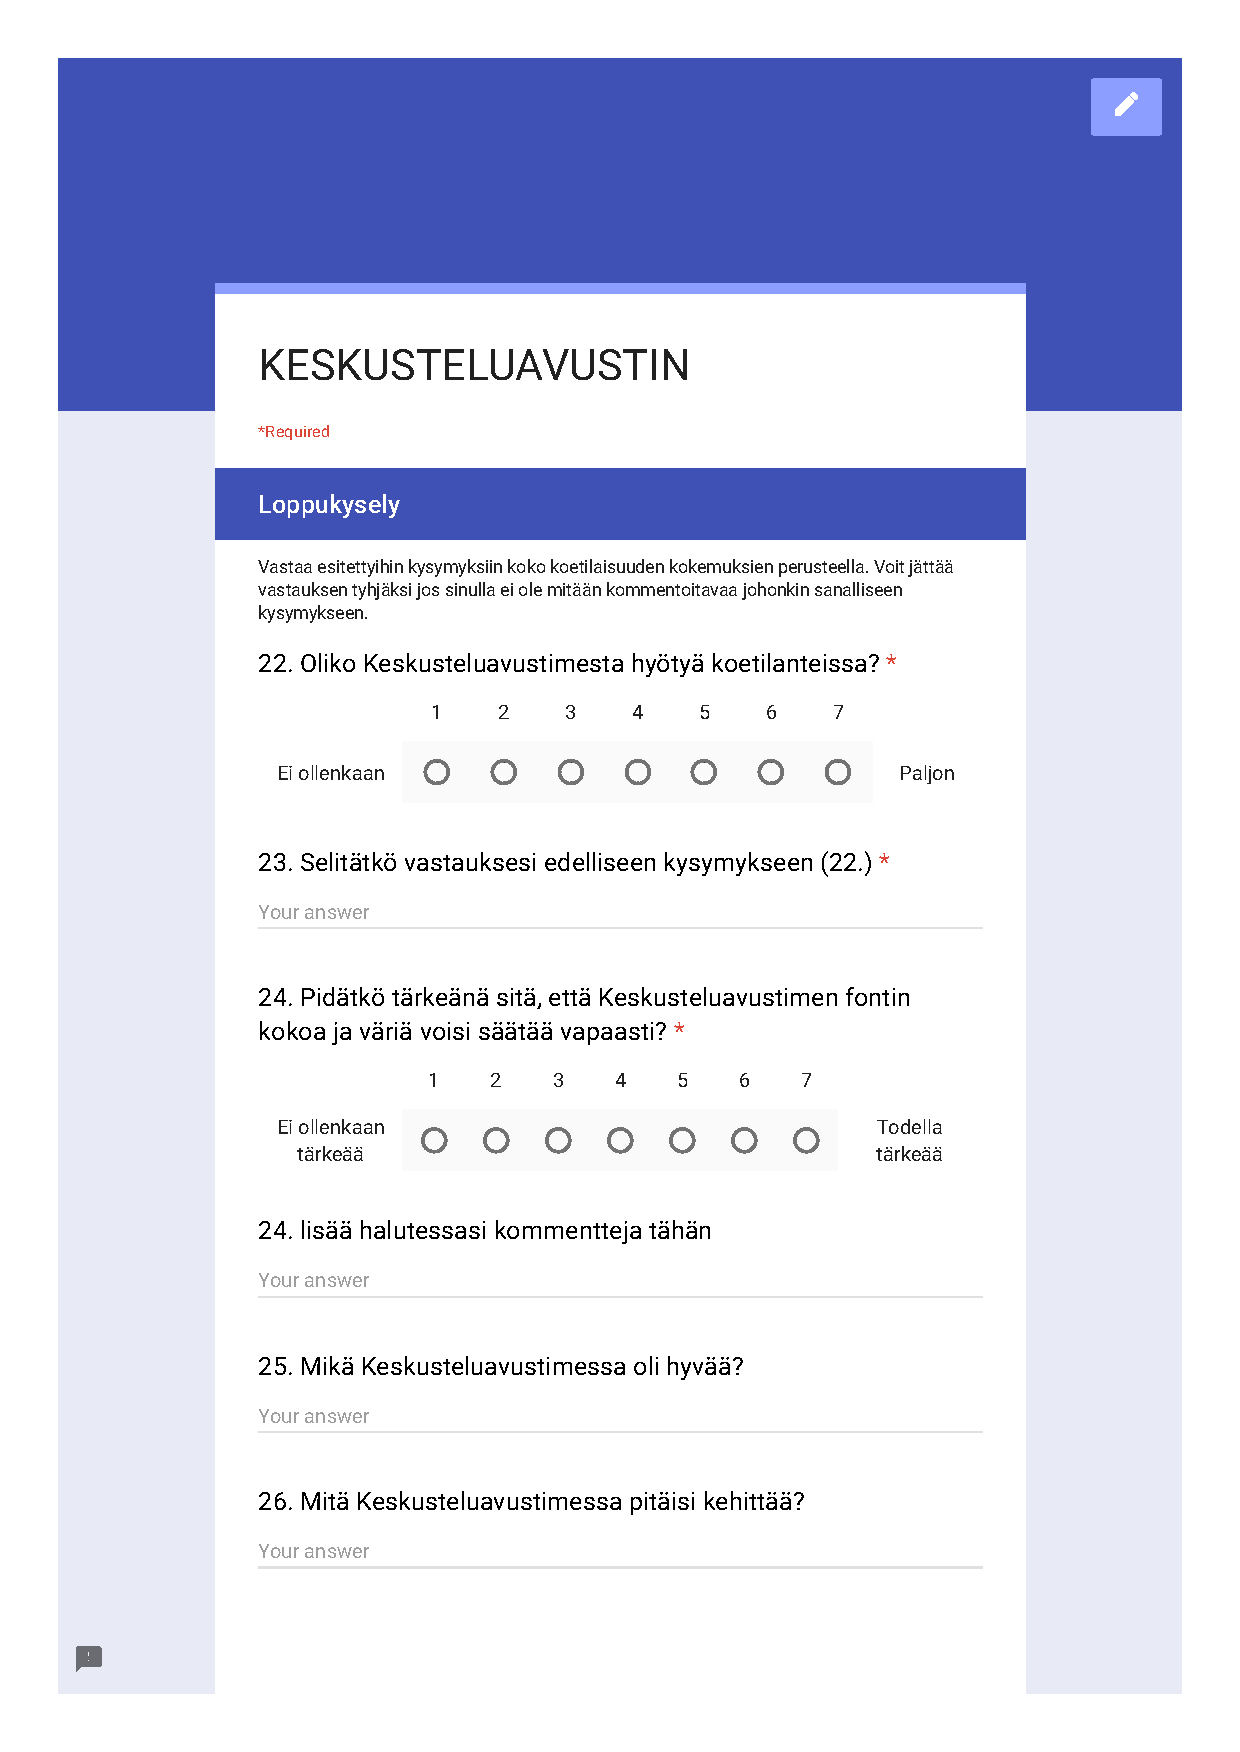
\includegraphics[page=1,trim={1cm 1cm 1cm 2.5cm}, clip, width=\textwidth]{q4.pdf}
\end{figure}
\begin{figure}
	\centering
	\includegraphics[page=2,trim={1cm 0cm 1cm 0cm}, clip, width=\textwidth]{q4.pdf}
\end{figure}
\begin{figure}
	\centering
	\includegraphics[page=3,trim={1cm 0cm 1cm 0cm}, clip, width=\textwidth]{q4.pdf}
\end{figure}

\section{Questionnaire Answers} \label{sec:answers}

The raw data from the user tests is included here. Each set of answers is identified by the number of the question, which corresponds to the number reported at the questionnaire listing in section \ref{sec:quest}. On the x-axis, P1 to P9 refer to the test participants. Values on the y-axis are the numerical answers on the scale from 1 to 7.

\begin{figure}[h!]
	\centering
	\begin{subfigure}[b]{0.49\textwidth}
		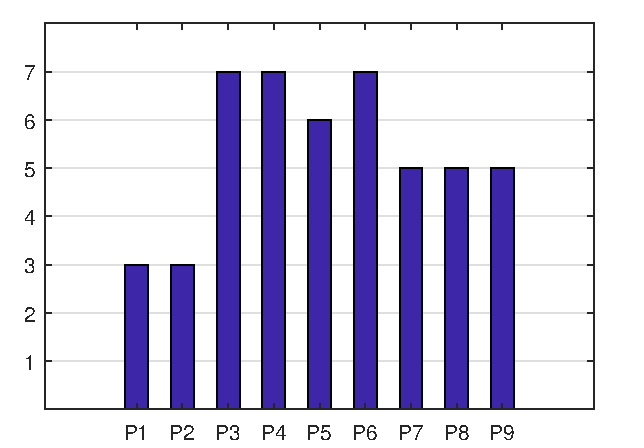
\includegraphics[width=\textwidth]{T2_1.pdf}
		\caption*{Q10}
	\end{subfigure}
	\begin{subfigure}[b]{0.49\textwidth}
		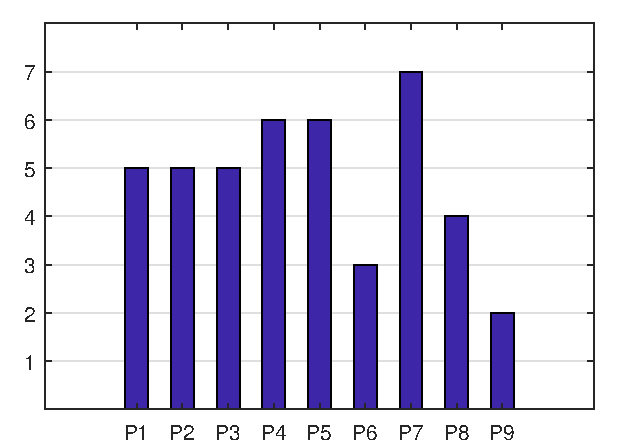
\includegraphics[width=\textwidth]{T2_2.pdf}
		\caption*{Q11}
	\end{subfigure}
	\begin{subfigure}[b]{0.49\textwidth}
		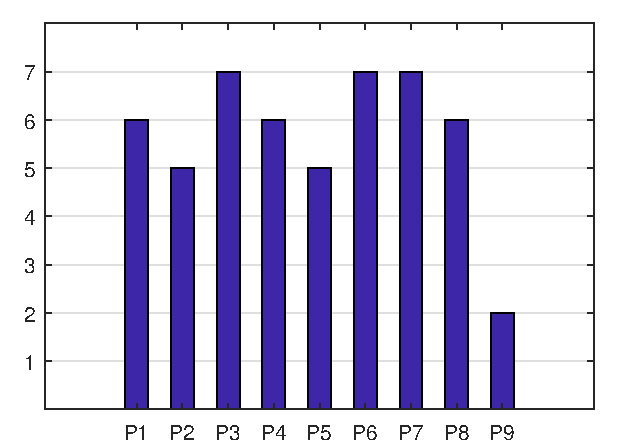
\includegraphics[width=\textwidth]{T2_3.pdf}
		\caption*{Q12}
	\end{subfigure}
	\begin{subfigure}[b]{0.49\textwidth}
		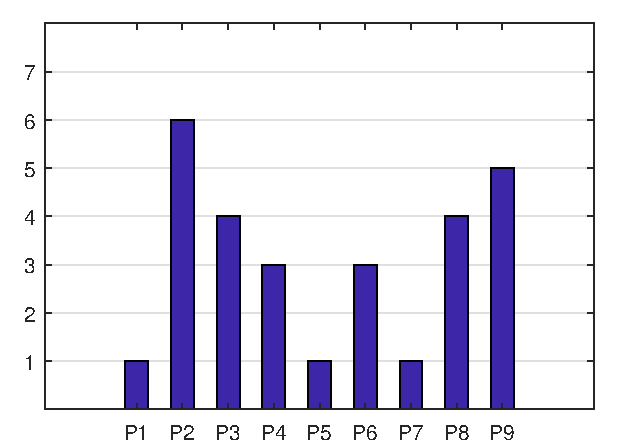
\includegraphics[width=\textwidth]{T2_4.pdf}
		\caption*{Q13}
	\end{subfigure}
	\begin{subfigure}[b]{0.49\textwidth}
		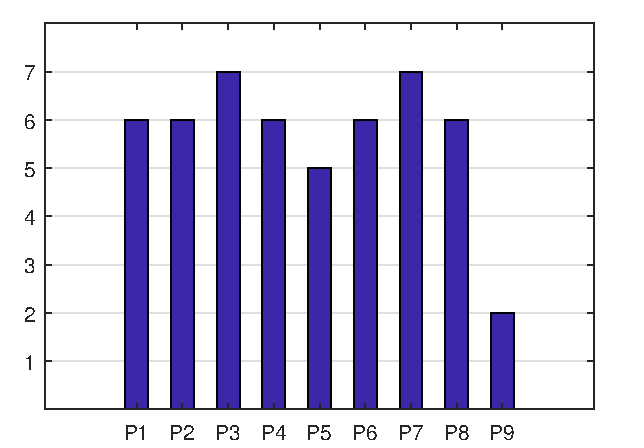
\includegraphics[width=\textwidth]{T2_5.pdf}
		\caption*{Q14}
	\end{subfigure}
	\begin{subfigure}[b]{0.49\textwidth}
		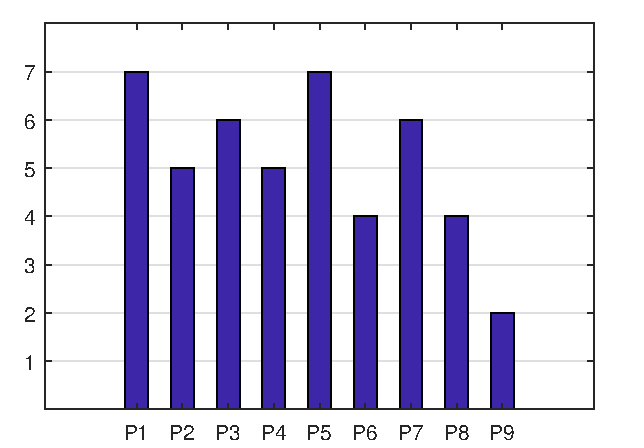
\includegraphics[width=\textwidth]{T2_6.pdf}
		\caption*{Q15}
	\end{subfigure}
	%\caption{Introduction and section 1 results.}
	%\label{fig:data} 
\end{figure}

\begin{figure}[h!]
	\centering
	\begin{subfigure}[b]{0.49\textwidth}
		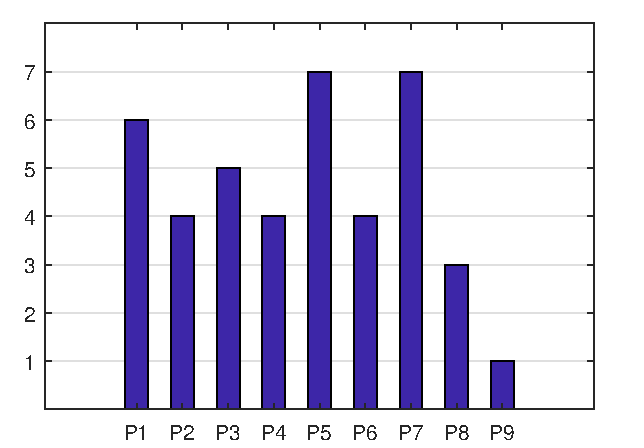
\includegraphics[width=\textwidth]{T2_7.pdf}
		\caption*{Q16}
	\end{subfigure}
	\begin{subfigure}[b]{0.49\textwidth}
		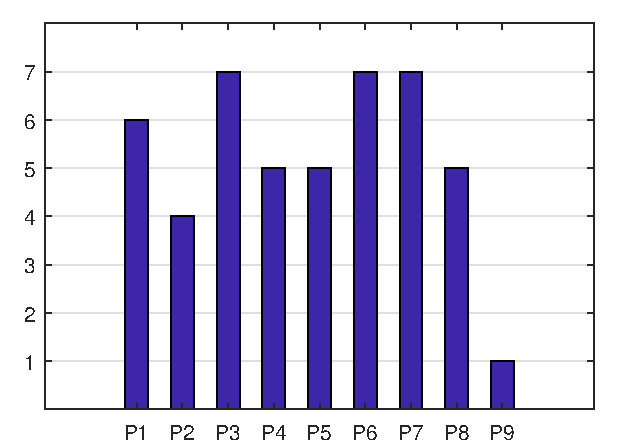
\includegraphics[width=\textwidth]{T2_8.pdf}
		\caption*{Q17}
	\end{subfigure}
	\begin{subfigure}[b]{0.49\textwidth}
		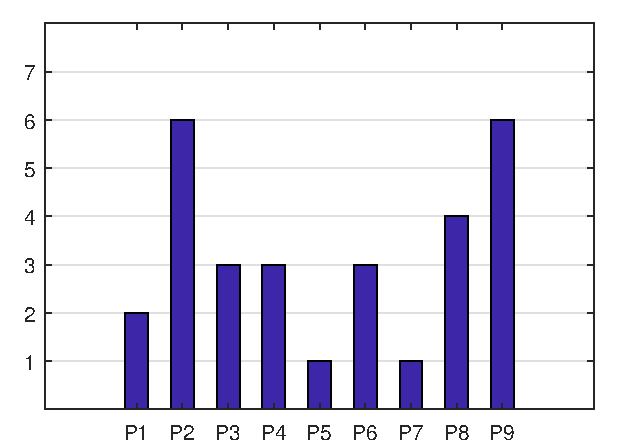
\includegraphics[width=\textwidth]{T2_9.pdf}
		\caption*{Q18}
	\end{subfigure}
	\begin{subfigure}[b]{0.49\textwidth}
		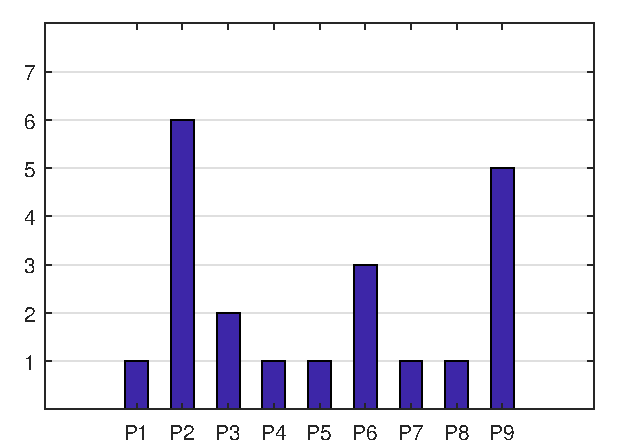
\includegraphics[width=\textwidth]{T2_10.pdf}
		\caption*{Q19}
	\end{subfigure}
	\begin{subfigure}[b]{0.49\textwidth}
		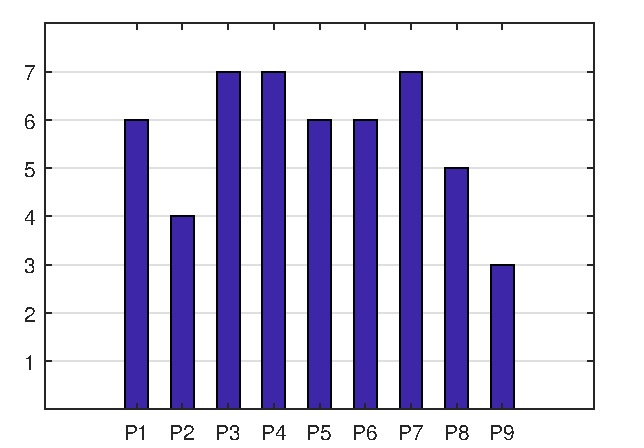
\includegraphics[width=\textwidth]{T2_11.pdf}
		\caption*{Q20}
	\end{subfigure}
	\begin{subfigure}[b]{0.49\textwidth}
		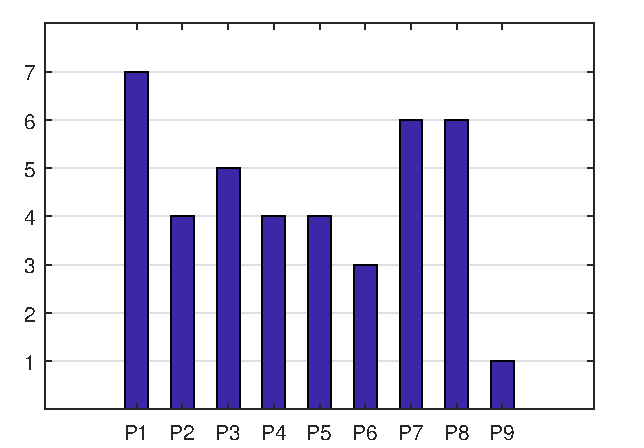
\includegraphics[width=\textwidth]{T2_12.pdf}
		\caption*{Q21}
	\end{subfigure}
	\begin{subfigure}[b]{0.49\textwidth}
		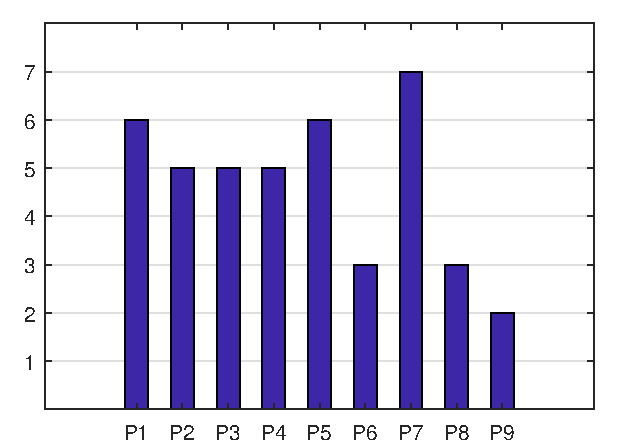
\includegraphics[width=\textwidth]{T2_13.pdf}
		\caption*{Q22}
	\end{subfigure}
	\begin{subfigure}[b]{0.49\textwidth}
		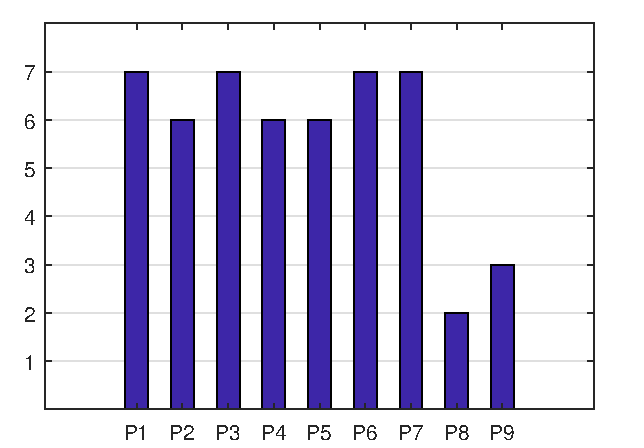
\includegraphics[width=\textwidth]{T2_14.pdf}
		\caption*{Q23}
	\end{subfigure}
	%\caption{Section 2 and debriefing results.}
	%\label{fig:data2} 
\end{figure}

\clearpage

\section{MATLAB Code} \label{sec:matlab}

This section presents the MATLAB scripts created for analyzing the user test results and producing most of the figures presented in this thesis.

\lstset{
	language=matlab,
	basicstyle=\ttfamily\scriptsize, % \tiny 
	inputencoding=utf8,
	extendedchars=true,
}

\subsection*{results.m}
\vspace{-4mm}
\lstinputlisting{results.m}
\vspace{8mm}
\subsection*{audiosignal.m}
\vspace{-4mm}
\lstinputlisting{audiosignal.m}
\vspace{8mm}
\subsection*{bformat.m}
\vspace{-4mm}
\lstinputlisting{bformat.m}
\vspace{8mm}
\subsection*{cepstrum.m}
\vspace{-4mm}
\lstinputlisting{cepstrum.m}
\vspace{8mm}
\subsection*{gmm.m}
\vspace{-4mm}
\lstinputlisting{gmm.m}
\vspace{8mm}
\subsection*{filterbank.m}
\vspace{-4mm}
\lstinputlisting{filterbank.m}
\vspace{8mm}
\subsection*{loudness.m}
\vspace{-4mm}
\lstinputlisting{loudness.m}

\end{document}
